\chapterillustration{./abertura-transformacoes}{./abertura-transformacoes-professor}

\expandtocdepth

\chapterwhat{Transformações geométricas no plano:
isometrias: translações, rotações e reflexões;	homotetias.}

\chapterbecause{Estamos mergulhados em um mundo de imagens, especialmente na atualidade, em função da multiplicidade de telas que manuseamos e às quais somos expostos. Apropriar-se do conceito de transformação geométrica, que está por detrás das noções de congruência, de simetria, de ampliação e de redução de imagens configura uma espécie de alfabetização geométrico-visual. Em resumo, o estudo das transformações geométricas contribui para a atuação no mundo por meio das linguagens geométrico-visuais presentes nas artes, nas ciências, nas tecnologias e na natureza.} 

\chapter{Transformações Geométricas}
\label{transformacoes-chap}


%%%% Página de créditos

% Autores
\autorum{Aline Matheus}
\autordois{Cláudia Cueva}

% Revisores
\revisorum{Lhaylla Crissaf}

\autordacapa{Patrick Hendry}{Unsplash}{https://unsplash.com/photos/hezNrE5QEa8}
\versao{1.0}


\creditos


\mainmatter

\begin{apresentacao}{Introdução}
\subsection{Objetivos gerais}

Os objetivos gerais a seguir expressam, de forma sintética, as aprendizagens relacionadas ao tema da unidade, que se espera alcançar como resultado do desenvolvimento dos objetivos específicos de cada seção, na forma e nos contextos implementados. 
\begin{itemize}
\item Associar as noções de congruência e semelhança, estudadas no Ensino Fundamental, às de isometria e homotetia.
\item Ampliar a capacidade de perceber, apreciar esteticamente e descrever elementos naturais ou produções humanas diversas por meio da linguagem associada às transformações geométricas.
\item Associar as isometrias aos movimentos de translação, reflexão e rotação. 
\item Relacionar isometrias e simetrias, reconhecendo a importância desta última noção para a organização do mundo físico e para as produções humanas.
\item Elaborar, analisar e testar conjecturas sobre os efeitos da composição de isometrias e homotetias, ampliando a capacidade de argumentar matematicamente. 
\item Analisar e construir figuras planas diversas utilizando as transformações geométricas.
\item \textbf{Conceitos abordados}: congruência, semelhança, isometria, simetria e homotetia.
\end{itemize}

\paragraph{Habilidades da BNCC}
\begin{habilities}{EM13MAT105}
Utilizar as noções de transformações isométricas (translação, reflexão, rotação e composições destas) e transformações homotéticas para construir figuras e analisar elementos da natureza e diferentes produções humanas (fractais, construções civis, obras de arte, entre outras).
\end{habilities}



\subsection{Sobre pré-requisitos e progressão das aprendizagens}
Na BNCC do Ensino Fundamental, os conceitos citados estão contemplados desde os anos iniciais de escolarização. O reconhecimento de figuras congruentes usando sobreposição, malhas e mesmo tecnologias digitais é tratado a partir do 3° ano e a habilidade a ser desenvolvida (\textbf{EF03MA16}) envolve a compreensão de que figuras congruentes têm a mesma forma e o mesmo tamanho, ainda que estejam em posições diferentes. No 4° ano, encontramos a habilidade (\textbf{EF04MA19}) que prevê reconhecer simetria de reflexão e utilizá-la na construção de figuras congruentes. Nos anos seguintes, encontram-se expressas as habilidades de reconhecer translações, rotações e reflexões e utilizá-las na construção de figuras planas (\textbf{EF07MA20}, \textbf{EF07MA21}, \textbf{EF08MA14}, \textbf{EF08MA18}). Também as ampliações e reduções em malhas quadriculadas ou com uso de tecnologias digitais e a construção de figuras semelhantes figuram entre as habilidades do ensino fundamental do 5° ao 9° ano (\textbf{EF05MA18}, \textbf{EF06MA21}, \textbf{EF06MA29}, \textbf{EF07MA19}, \textbf{EF09MA12}). 

Mesmo que a abordagem a esses conceitos esteja prevista no Ensino Fundamental pela BNCC, ela não é tomada de modo estrito, nesta unidade, como pré-requisitos. Em vez disso, procuramos revisitá-los ao mesmo tempo que os aprofundamos, procurando dar vida à ideia de um currículo espiral \citep{bruner1960,roldao1994}. Tal aprofundamento se dá em duas dimensões: contextual e conceitual. 

O aprofundamento contextual se caracteriza pela escolha de situações e temas que dialogam com a complexidade das obras humanas e do olhar humano sobre a natureza, contribuindo para ampliar o repertório cultural dos alunos e, ao mesmo tempo, valorizar a matemática como lente que permite ler o mundo. 

O aprofundamento conceitual se dá pela interconexão entre diferentes conceitos, pela exigência de explicações, previsões, e elaborações diversas com relação ao tema, sem, no entanto, apelar em demasia para o formalismo matemático. 

\textbf{Quantidade de aulas previstas para a unidade}: 17 horas/aula.

A Unidade aqui proposta é bastante extensa e caberá ao professor fazer algumas escolhas, tendo em vista as particularidades de suas turmas. 
	
Como dissemos anteriormente, a BNCC do Ensino Fundamental prevê o desenvolvimento de diversas habilidades ligadas às transformações. Entretanto, o currículo previsto não pode ser tomado como currículo praticado ou efetivamente “aprendido”. Dessa forma, é muito importante que o professor procure saber o que seus alunos já sabem e conseguem fazer com relação aos assuntos de cada seção. 
	
O primeiro “Explorando” de cada seção pode servir bem a esse diagnóstico. Uma vez que o professor observe que os alunos já têm certo nível de conhecimento sobre o tema, pode saltar para atividades mais avançadas, concentrando-se, em sala de aula, no “Organizando”, que visa a sistematizar os conceitos abordados. Convém nesse caso, usar um ou mais contextos presentes nos “Explorando” como motivação para o assunto, mas sem se preocupar em percorrer sistematicamente todas as atividades propostas. (Metodologias como sala de aula invertida ou rodízio por estações pode contribuir para abordar esses contextos de forma dinâmica e personalizada, de forma não linear.)

Se, por outro lado, o professor diagnosticar que seus alunos conhecem pouco sobre os conceitos abordados, talvez convenha priorizar o “Explorando” de cada seção, que traz atividades exploratórias, que visam ao desenvolvimento da capacidade de visualização relativa às transformações, mas não chegam a sistematizar os conceitos. 

Ainda sobre as escolhas que podem ser feitas, convém observar que as seções 1 a 3 relacionam-se às isometrias e estão bastante conectadas entre si. A seção 1 procura iniciar o assunto relacionando-o com o conceito de congruência – usualmente trabalhado no Ensino Fundamental mesmo antes da BNCC. As seções 2 e 3 são divididas para melhor tratar das especificidades de diferentes tipos de isometrias (translações, rotações e reflexões na seção 2 e simetrias na seção 3). Já a seção 4 depende pouco das demais e aborda as homotetias tomando o conceito de semelhança como ponto de partida.
\clearpage

\subsection{Diretrizes teóricas e metodológicas da unidade}
\paragraph{Sobre o objeto de estudo}

É comum a ideia de que, em Geometria, estudam-se propriedades de figuras geométricas. Quais propriedades? Em geral, consideramos as propriedades que são chamadas intrínsecas, isto é, aquelas que não dependem da localização das figuras geométricas no plano (ou dos objetos no espaço).  Duas figuras idênticas – ou seja, com as mesmas propriedades intrínsecas – e que ocupam posições diferentes são chamadas de congruentes. 

Congruência é um conceito tratado nesta unidade, mas não da forma tradicional. Estamos interessados nos deslocamentos – translações, rotações e reflexões que levam uma figura à outra congruente a ela, a fim de representar matematicamente a ideia de sobreposição. Especificamente, vamos nos debruçar primeiro sobre as transformações geométricas que relacionam figuras congruentes, as chamadas isometrias. 

O entendimento intuitivo das isometrias baseia-se na noção de movimentos rígidos, isto é, aqueles que não deformam, nem ampliam, nem reduzem as figuras geométricas. Partiremos dessa ideia para chegar à noção de isometria como transformação geométrica, ou seja, como uma função que associa pontos do plano a pontos do plano, de modo a manter inalteradas as distâncias entre eles. 

As isometrias relacionam-se intimamente à noção de simetria que, além de noção matemática, é uma ideia fortemente presente na cultura e na natureza. Matematicamente, dizemos que uma figura é simétrica se é invariante por alguma isometria particular, distinta da identidade.

As homotetias – que repousam sobre as ideias intuitivas de ampliação e redução, relacionando-se, assim, com a noção de semelhança – são transformações geométricas, de modo que serão também abarcadas pela unidade. 

\paragraph{Sobre a metodologia}
A construção da unidade não segue de forma estrita nenhuma linha teórica relativa ao ensino e à aprendizagem da Matemática e, em particular, da Geometria. Mas algumas diretrizes importantes foram consideradas pelas autoras e serão, agora, oportunamente, compartilhadas com os professores. Com isso, esperamos que os professores possam imprimir maior intencionalidade pedagógica à sua própria abordagem do capítulo.

Uma importante referência utilizada para nortear a construção da Unidade Temática é o chamado Modelo de Van Hiele. Trata-se de um modelo de ensino e aprendizagem de geometria apoiado em experiências educacionais do casal Van Hiele (1957)\footnote{falta a referência}.  O ponto central da teoria é que, no processo de aprendizagem de geometria, o raciocínio do indivíduo passa por cinco níveis sequenciais e ordenados. A compreensão e utilização de conceitos geométricos ocorre de maneiras específicas em cada nível, observáveis por meio das diferentes formas com que o estudante interpreta, define, classifica os conceitos em jogo e justifica, refuta ou demonstra as conjecturas que surgem no processo de aprendizagem.   

São propriedades do modelo a sequencialidade dos níveis, a linguagem específica em cada nível, a continuidade (processo gradual e paulatino da aquisição de um nível a partir do anterior) e a localidade (o indivíduo pode ter raciocínio compatível com um nível em determinado tópico e compatível com nível diferente em outro tópico de geometria).

A teoria de Van Hiele está construída sobre dois grandes pilares: o descritivo e o instrutivo.

\begin{itemize}
\item \textbf{Aspecto descritivo}. Classificação do raciocínio de um indivíduo, em seu aprendizado de geometria, em níveis:
\begin{enumerate}[label=\titem{\Roman*)}]
\item Visualização/Reconhecimento, 
\item Análise,
\item Classificação/Dedução Informal,
\item Dedução Formal,
\item Rigor. 
\end{enumerate}

É interessante destacar que, \citet{pastor1993}, entre outros autores, indica que, para a Educação Básica, o esperado é que os estudantes atinjam o nível III, da dedução informal, que se caracteriza por operações cognitivas tais como: compreender, classificar, aplicar, predizer, conjecturar e generalizar. Nesse nível, o estudante expressa tais operações utilizando linguagens que ainda não são aquelas próprias da matemática acadêmica, mas que já sinalizam alguma consciência dos problemas relacionados à generalização. 

\item \textbf{Aspecto instrutivo}. Os Van Hiele concluíram que o progresso de um nível ao seguinte depende mais da instrução recebida do que da idade ou da maturidade do aluno e, para orientar os professores na elaboração do planejamento para a sala de aula, propuseram cinco \textit{fases de aprendizagem}. Eles afirmam que a instrução assim empregada promove o desenvolvimento completo dos alunos dentro de um certo nível, tornando-os aptos a avançar para o próximo. 
Essas fases de aprendizagem são: 

\begin{enumerate}[label=\titem{\arabic*.}]
\item \textbf{Fase da informação}. Caracteriza-se por um movimento de mão dupla: o professor vai perguntando aos alunos o que eles sabem sobre o assunto e vai esclarecendo os termos referentes ao que se vai estudar.
\item \textbf{Fase da orientação dirigida}. O professor oferece tarefas que levam o aluno a atingir os objetivos do nível, interagindo continuamente com eles.
\item \textbf{Fase da explicitação}. Marcada pelos diálogos entre duplas, alunos e professor e até toda a turma. Durante as discussões sobre cada tema proposto, cabe ao professor conduzir a turma para o correto entendimento dos conceitos e resultados tratados e cuidar do uso da linguagem, de forma que o vocabulário dos alunos vá sendo ampliado no decorrer das atividades.  Modernamente, recomenda-se que o diálogo esteja presente em todo o trabalho, deixando assim de ser uma fase para transformar-se numa forma de condução do processo de ensino.
\item \textbf{Fase da orientação livre}. O professor propõe desafios e quase não interfere, deixa que os alunos os enfrentem de forma autônoma. 
\item \textbf{Fase da integração}. Nesta fase, o professor deve conduzir os alunos para que façam uma síntese do que aprenderam (no nível), falando ou escrevendo.  Além disso, este é um momento em que o professor elabora e apresenta aos alunos, de modo organizado e claro, um resumo do conjunto de conceitos e resultados estudados até então, de modo a validá-los. É fase muito importante para sanar as dúvidas e corrigir algum equívoco que reste na compreensão dos alunos sobre o tema tratado.  
\end{enumerate}

\end{itemize}
Em resumo, o trabalho do professor é o de estimular o protagonismo de seus alunos: o aluno traz informações sobre um assunto, é provocado por novas informações e atividades oferecidas pelo professor, faz questionamentos, discute, é orientado pelo professor até chegar às suas conclusões e, finalmente, expressá-las. 

É importante sinalizar que o Modelo de Van Hiele não é tomado de forma rígida na Unidade, estabelecendo este ou aquele nível nas seções que se seguem. Além disso, as fases de aprendizagem são usadas como norteadoras nas escolhas das atividades propostas, mas não de forma exclusiva. Dentro da unidade temática outros recursos aparecem como estratégias de aprofundamento das aprendizagens.

Como referência essencial, o Modelo de Van Hiele dá, a nós professores, diretrizes importantes a seguir em nosso planejamento do ensino de Geometria (ou até de outros tópicos), tais como: 

\begin{itemize}[itemsep=0pt, topsep=0pt]
\item Levar em conta as informações que os alunos trazem sobre o assunto a ser tratado;
\item Cuidar da adequação da linguagem, que deve evoluir gradativamente em profundidade e formalidade;
\item Aumentar continuamente, sem saltos abruptos, a profundidade das aprendizagens, considerando diferentes tipos de operações cognitivas sobre os objetos de conhecimento em jogo;
\item Considerar que a progressão das aprendizagens ocorre localmente, isto é, dentro de um mesmo assunto.
\end{itemize}

\paragraph{Sobre obstáculos à aprendizagem no assunto}
Em trabalhos sobre ensino de isometrias algumas dificuldades foram observadas, entre alunos da Educação Básica, nas tarefas de reconhecimento da transformação geométrica aplicada a uma figura \citep[Bautier, 1986\footnote{falta a referência}][]{grenier1988,cona2017} (Bautier, 1986; Grenier, 1988; Cona, 2017).  Foram identificados erros recorrentes nas questões em que a posição do vetor de translação em relação à figura dada, ou a posição do centro de rotação em relação à figura dada ou{} a reta de reflexão em relação à figura dada não eram usuais (horizontais, verticais); ou ainda questões em que os elementos estavam sobrepostos (centro de rotação em um ponto interior à região limitada pela figura a ser rotacionada ou reta de reflexão contendo pontos da figura a ser refletida).  Também foram observadas dificuldades em situações em que não existe ortogonalidade ou paralelismo entre elementos da figura e o eixo de reflexão ou aquelas em que o eixo de simetria contém pontos da figura em questão.

Acredita-se que essas dificuldades têm origem em etapas anteriores da escolarização, em que o aluno elaborou concepções limitadas de que, por exemplo, a reflexão em relação a uma reta sempre está associada à presença de duas figuras, uma de cada lado de um eixo de simetria explícito. Concepções limitadas também podem estar relacionadas ao ensino tradicional de congruências (e, também, de semelhanças), que muitas vezes se resume à apresentação de “casos de congruência de triângulos”, conteúdo cuja abordagem está bastante arraigada na cultura escolar, e à proposta de exercícios repetitivos que não trazem desafios. 

Nesta unidade pretendemos que as tarefas propostas tenham potencial para tirar o estudante da zona de conforto e desestabilizar concepções errôneas a fim de quebrar obstáculos no aprendizado de transformações geométricas e aumentar a compreensão sobre o tema. O professor será alertado, no decorrer das seções, para o tipo de dificuldade que pode aparecer e estimulado a fazer intervenções que propiciem a evolução do raciocínio do aluno.

\end{apresentacao}

\begin{paginatexto}{Seção 1 - Congruência}
\subsection{Objetivo geral da seção}
\begin{itemize}
\item Compreender a noção de congruência, identificando, inclusive, os movimentos que permitem associar duas ou mais figuras planas congruentes.
\end{itemize}

\textbf{Quantidade de aulas previstas para a seção}: 3 horas/aula.

\subsection{Enriquecimento da discussão}
A congruência entre figuras é tema bastante explorado na Educação Básica, em que aparece com forte ligação à sobreposição de figuras. Nesta seção, o objetivo é articular o conceito de congruência aos movimentos que permitem sobrepor uma figura à outra. O assunto deve ser abordado, de acordo com a BNCC, desde os anos iniciais do Ensino Fundamental (\textbf{EF03MA16}) a partir da ideia de que duas figuras são congruentes se podem ser sobrepostas e que, consequentemente, têm a mesma forma e o mesmo tamanho e, inclusive a mesma área (\textbf{EF03MA21}). Também a noção de simetria de reflexão é proposta cedo (\textbf{EF04MA19}), com ênfase explícita à propriedade de manutenção de forma e do tamanho de figuras simétricas e estímulo à construção de figuras congruentes por meio de reflexões.  Os alunos devem ter tido oportunidade de retomar, conforme previsto para o 7° ano, as simetrias de reflexão (em relação aos eixos e à origem) e de conhecer as demais transformações geométricas que não alteram a forma ou o tamanho das figuras: a translação, a reflexão em relação a uma reta e a rotação com centro em um ponto (\textbf{EF07MA20}, \textbf{EF07MA21}). No 8° ano, estão contempladas as construções de figuras obtidas pela aplicação das transformações geométricas ou de composições delas (\textbf{EF08MA18}). No entanto, não assumimos tais conceitos como pré-requisitos estritos do estudo a desenvolver, pois nesta seção eles serão retomados em diversos contextos que favoreçam sua articulação e aprofundamento. 

Ainda que os alunos tenham tido contato com a noção de congruência somente sob um ponto de vista tradicional, em que se dá grande ênfase aos casos de congruência de triângulos (\textbf{EF08MA14}), a ideia aqui é explorar a relação entre a congruência de figuras e as transformações geométricas que permitem representar a sobreposição de uma figura a outra. Ou seja, estamos interessados nos movimentos – translações, rotações e reflexões – que associam uma figura a outra congruente a ela.

Ao arrastar um móvel em linha reta, ao mudar um quadro de lugar na parede ou ao abrir uma gaveta realizamos movimentos de translação. É claro que o quadro na nova posição é congruente ao quadro na posição original. Dizemos que um ponto marcado na gaveta aberta é a translação do ponto em sua posição original, quando a gaveta estava fechada. Fazemos um movimento de rotação ao abrirmos uma porta e observamos que, em um par de sapatos, cada pé é refletido do outro. De modo geral, desde os deslocamentos permitidos em um jogo de xadrez até a arrumação de objetos em um armário, efetuamos uma sucessão de movimentos rígidos, isto é, movimentos que não alteram forma ou tamanho dos objetos.

Nesta seção, as noções de translação, rotação e reflexão ainda não serão formalizadas. A ideia é o seu reconhecimento e sua descrição de modo informal. Por exemplo, a translação de uma figura no plano corresponde a um movimento retilíneo e podemos pensar que o deslocamento da figura é feito em um trilho reto, formado por duas retas paralelas; a rotação de uma figura no plano corresponde ao deslocamento circular como se ela estivesse presa na ponta de um ponteiro de relógio; a ideia de reflexão é a de que uma figura é a imagem de outra refletida em um espelho plano. As discussões durante a execução das atividades propostas devem permitir, inclusive, que o professor faça um diagnóstico das concepções dos alunos associadas a esses movimentos.

\subsection{Organização da turma}
Cada aluno deve ser convidado a ler as atividades propostas e refletir um pouco sobre elas para, então, trabalhar em dupla ou grupo; é importante para o desenvolvimento do raciocínio dos alunos que eles explicitem suas ideias e discutam com seus colegas sobre as perguntas que surgem naturalmente na execução das tarefas. 

\subsection{Sobre as atividades da seção}
São atividades de reconhecimento visual de figuras congruentes em que a prioridade é descrever informalmente as transformações geométricas que permitem sobrepor uma figura à outra. Não se trata de demonstrar a congruência de figuras por meio de técnicas conhecidas na geometria, como, por exemplo, casos de congruência de triângulos. Nessa primeira seção, as isometrias não são formalmente definidas, mas o professor deve ficar atento para o emprego correto dos termos translação, rotação e reflexão para permitir que os alunos expressem a diversidade de ideias que as atividades podem suscitar. Alguns estudantes terão mais facilidade do que outros no decorrer do trabalho prático com os anexos fornecidos nas atividades e o professor pode propor o uso de material concreto ou de desenho – régua, esquadro, discos, transferidor, espelhos – para facilitar a compreensão dos movimentos de translação, rotação e reflexão em relação a uma reta. 
\end{paginatexto}

\explore{Congruência?}
\clearmargin
\begin{sugestions}{Movimentos e congruências no Tetris}
{

\textbf{Material necessário}: malha quadriculada

A atividade deve ser vista como um diagnóstico que permite descobrir quais são os significados que os alunos atribuem aos termos, para poder compreender suas referências e estabelecer uma linguagem comum sobre os assuntos que estão começando a ser estudados. Particularmente o item a, propicia um momento de informação de mão dupla em que, inicialmente, os alunos trarão seu entendimento informal sobre os termos citados. Alguns estudantes podem mencionar que já estudaram congruência de triângulos e esse conhecimento deve ser bem explorado lembrando que figuras congruentes, a exemplo dos triângulos congruentes, têm a mesma forma e o mesmo tamanho. Também podem se lembrar do movimento de translação da Terra em torno do Sol; se isso ocorrer será necessário esclarecer que a Terra percorre uma órbita elíptica em torno do Sol e que as translações a serem estudadas aqui são os deslocamentos retilíneos entre dois pontos.   Não se trata tanto de “corrigi-los”, mas de compreender suas referências e explicitar os significados dos termos dentro do estudo pretendido (ainda que de modo informal neste primeiro momento). As discussões durante a execução dos itens propostos devem permitir, inclusive, que o professor faça um diagnóstico das concepções dos alunos associadas a esses movimentos. Até o fim da atividade, cabe ao professor garantir a compreensão de que a translação de uma figura no plano corresponde a um movimento retilíneo entre dois pontos e podemos pensar que o deslocamento da figura é feito em um trilho reto, formado por duas retas paralelas; a rotação de uma figura no plano corresponde ao deslocamento circular em torno de um ponto, como se ela estivesse presa na ponta de um ponteiro de relógio; a reflexão espelha todos os pontos de uma figura em relação a uma reta, exatamente como ocorre com a imagem refletida em um espelho plano. 
}{1}{2}
\end{sugestions}
\begin{answer}{Movimentos e congruências no Tetris}
{
\begin{enumerate}
\item Espera-se que os alunos, a partir de suas pesquisas ou por meio de exemplos, associem o termo congruência à manutenção de forma e tamanho. Associem translação a situações em que há deslocamento retilíneo entre dois pontos e rotação a movimentos circulares. 
\item Apenas R.

\end{enumerate}
}{1}
\end{answer}
\begin{sugestions}{Movimentos e congruências no Tetris}
{
\paragraph{Sugestão de condução}

Os alunos podem pensar e fazer registros sobre os itens \titem{a)} até \titem{e)} em duplas. A seguir, esses itens podem ser discutidos em plenária. A ideia é usar a discussão em plenária para diagnosticar o entendimento dos alunos sobre o conceito de congruência, bem como sua fluência e vocabulário para identificar e descrever os movimentos com as peças do Tetris. A partir daí, o professor pode conduzir os alunos para o uso das palavras rotação, translação e reflexão. O item \titem{e)} é especialmente relevante, porque os pares de peças R/L e S/Z são congruentes, mas não podem ser sobrepostos pelos movimentos permitidos no jogo. Podem, entretanto, ser sobrepostos por um movimento no espaço, que resulta na reflexão das formas, que eles podem compreender a partir da noção intuitiva de espelhamento. 

O item \titem{f)} pode ser realizado em duplas, usando malha quadriculada. O professor pode circular pela classe estimulando os alunos a examinar se não estão contabilizando repetidas vezes os mesmos triminós e pentaminós, por meio da visualização de suas rotações e reflexões. 

O item \titem{g)} pode ser apresentado como um desafio livre extraclasse. Tal desafio permite exercitar intensamente a visualização geométrico-espacial, em especial exigindo a imaginação dos movimentos que são a base intuitiva desta unidade. Convém valorizar o engajamento dos alunos que se dedicarem ao desafio, dando espaço, em aulas posteriores, não apenas para as soluções corretas, mas também para a discussão de tentativas, dificuldades e ideias que surgiram no processo. O importante é que os alunos sintam que erros e dificuldades não correspondem a fracasso, mas são parte de um processo de construção de conhecimento que pode se beneficiar de discussões coletivas.
}{1}{1}
\end{sugestions}
\begin{answer}{Movimentos e congruências no Tetris}
{
\begin{enumerate}\setcounter{enumi}{2}
\item Espera-se que os alunos digam (com estímulo do professor, se necessário) que a peça deve sofrer uma rotação em sentido horário ou anti-horário, de $90^{\circ}$. Nesse momento, ainda não se espera que seja descrito o centro da rotação. 
\item Pares congruentes: R e L; S e Z.
\item Não é possível fazer a sobreposição entre os pares congruentes usando os movimentos do jogo. As figuras são refletidas ou, usando uma linguagem mais técnica, são enantimorfas. A intuição física é justamente que só poderíamos sobrepor essas figuras usando um movimento no espaço. O efeito é o de um espelhamento. 
\end{enumerate}
}{1}
\end{answer}
\begin{answer}{Movimentos e congruências no Tetris}
{
\begin{enumerate}\setcounter{enumi}{5}
\item 2 triminós; 12 pentaminós.
\begin{figure}[H]
\centering

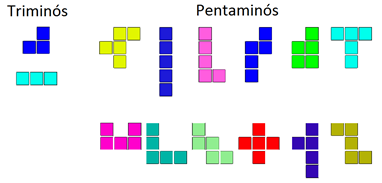
\includegraphics[width=.7\linewidth]{transformacoes6}
\end{figure}

\item Para esse desafio, utilizar material disponibilizado no Anexo 1. Resposta possível:
\begin{figure}[H]
\centering

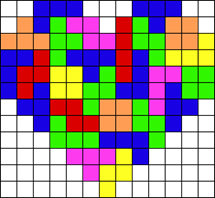
\includegraphics[width=.35\linewidth]{transformacoes7}
\end{figure}
\end{enumerate}
}{0}
\end{answer}

Você conhece o jogo Tetris? 

O Tetris é um dos jogos eletrônicos abstratos mais famosos do mundo! Ele foi criado pelos engenheiros Alexey Pajitnov e Dmitry Pavlosvsky, do Centro de Computadores da Academia Russa de Ciências, tendo sido lançado comercialmente em 1984. 

No Tetris, os jogadores devem organizar peças de quebra-cabeça em tempo real, enquanto caem do topo do campo de jogo, usando movimentos de \textbf{translação} ou \textbf{rotação}. Os jogadores devem tentar eliminar o maior número possível de linhas, o que é feito completando linhas horizontais de blocos sem espaço vazio. Se as peças se acumularem até o topo do tabuleiro eletrônico, o jogo acabou. 

\begin{figure}[H]
\centering

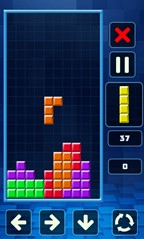
\includegraphics[width=.4\linewidth]{transformacoes1}
\end{figure}

Pode parecer simples, mas a popularidade do jogo demonstra o quanto ele é atraente. No site oficial do jogo, seus desenvolvedores dizem que “\textit{o Tetris, como o mundo real, desafia os jogadores a ordenar o caos usando um sistema organizacional específico, os componentes do jogo se traduzem facilmente em interpretações de situações reais da vida. Esteja você carregando a mala do carro, carregando uma máquina de lavar louça ou organizando as prateleiras, provavelmente está pensando em como cada objeto se encaixará estrategicamente com o mínimo de espaço vazio}”.

O design do jogo utiliza sete peças geométricas distintas, que são tetraminós, figuras compostas por quatro quadrados congruentes que se unem por meio de lados comuns. O prefixo “tetra” (que vem do grego) indica que os tetraminós são formados por quatro quadrados. 

\begin{figure}[H]
\centering

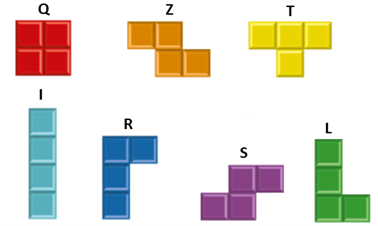
\includegraphics[width=.7\linewidth]{transformacoes2}
\caption{As sete peças do jogo Tetris. Saiba mais sobre o jogo e experimente jogar acessando: \url{https://tetris.com/play-tetris/}.}
\end{figure}

O Tetris é um jogo que se relaciona a diversos conceitos da Geometria. Um aspecto particular que podemos explorar diz respeito à noção de congruência, que você já estudou no Ensino Fundamental. Nas atividades que seguem, você terá chance de relembrar e aprofundar sua compreensão desse conceito.

\begin{task}{Movimentos e congruências no Tetris}
\begin{enumerate}
\item No texto sobre o jogo Tetris, há algumas palavras em destaque: \textbf{translação}, \textbf{rotação} e \textbf{congruente}. Você sabe o que essas palavras significam? Se não souber, pesquise e troque informações com seus colegas. Registre por escrito o significado de cada uma dessas palavras segundo seu próprio entendimento.
\item Analise a situação de jogo a seguir.
\begin{figure}[H]
\centering

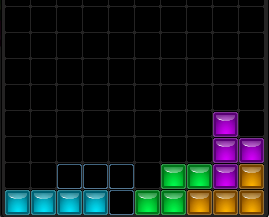
\includegraphics[width=.475\linewidth]{transformacoes3}
\end{figure}

Qual peça poderia ser encaixada no espaço demarcado? L, R, ambas ou nenhuma delas?
\item Analise esta outra situação de jogo.
\begin{figure}[H]
\centering

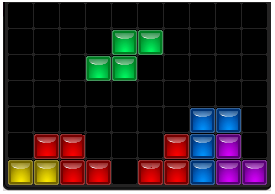
\includegraphics[width=.45\linewidth]{transformacoes4}
\end{figure}

Que movimento deve ser feito com a peça S para que ela seja encaixada no espaço imediatamente abaixo dela cumprindo os objetivos do jogo?

\item Entre as peças do jogo Tetris, existem pares de figuras congruentes. Quais são esses pares e por que tais figuras são congruentes? Desenhe os pares de figuras congruentes e explique.

\item Considere os pares de figuras congruentes que você identificou no item anterior. É possível sobrepor essas peças usando apenas os movimentos permitidos no jogo? Se sim, descreva como poderia ser feita a sobreposição. Se não, explique o porquê.

\item Há cinco tetraminós diferentes, embora haja sete peças de Tetris, porque, para contá-los, consideramos os congruentes como iguais. Para além do jogo Tetris, existem também outros tipos de minós: monominós, dominós, triminós, pentaminós etc, a depender da quantidade de quadrados utilizados. Quantos são os triminós? E os pentaminós? (Para realizar essa atividade, use uma malha quadriculada.)

\item Desafio: usando apenas as formas das peças de Tetris, será que você consegue completar o coração quadriculado abaixo, sem deixar nenhum espaço vazio e sem fragmentar nenhuma forma? Use lápis coloridos e as figuras disponibilizadas no \textbf{Anexo 1} para fazer suas tentativas.

\begin{figure}[H]
\centering

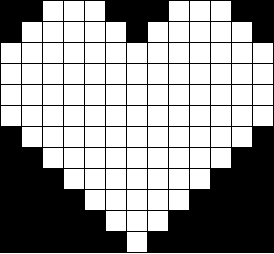
\includegraphics[width=.4\linewidth]{transformacoes5}
\end{figure}
\end{enumerate}
\end{task}

\arrange{Congruência}

É comum a ideia de que, em Geometria, estudam-se propriedades de figuras geométricas. Por exemplo, dado um triângulo retângulo cujos catetos medem 3 e 4 unidades, o resultado conhecido como Teorema de Pitágoras nos garante que a hipotenusa desse triângulo mede 5 unidades. Essa é uma propriedade desse triângulo que não depende de sua localização no plano. 

Mas podemos dizer que dois triângulos retângulos de lados 3, 4 e 5 unidades são “\textit{o mesmo triângulo”}? É evidente que, quando levamos em conta não apenas as propriedades de uma figura como essa, mas também a sua localização, não podemos dizer isso. Duas figuras idênticas em forma e tamanho – isto é, que podem ser sobrepostas sem faltar e sem sobrar nada –, mas que ocupam posições diferentes são chamadas de \textbf{congruentes}. 

A noção de congruência é tratada no Ensino Fundamental, de modo que você já pode ter entrado em contato com estratégias para reconhecer se duas figuras são congruentes ou não. Em geral, são apresentados casos de congruência de triângulos: Lado-Ângulo-Lado (LAL); Lado-Lado-Lado (LLL), Ângulo-Lado-Ângulo (ALA) etc. Essa abordagem é útil na dedução de muitos resultados geométricos e, também, na resolução de diversas questões envolvendo triângulos e outros polígonos.

Quando as figuras congruentes são polígonos, pode ser útil reconhecer vértices e lados \textbf{correspondentes} ou \textbf{homólogos}. Vamos analisar os polígonos $ABCDE$ e $MNOPQ$ da \fref{transformacoes8}: 

\begin{figure}[H]
\centering

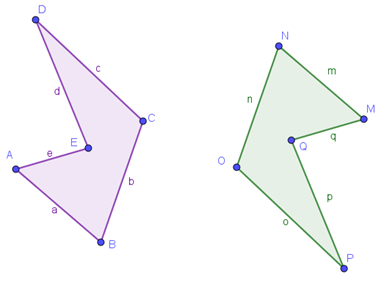
\includegraphics[width=.6\linewidth]{transformacoes8}
\caption{}
\label{transformacoes8}
\end{figure}

Na \fref{transformacoes8}, os pentágonos $ABCDE$ e $MNOPQ$ são congruentes e o vértice $A$ é homólogo ao vértice $M$, $B$ é homólogo ao $N$, e assim por diante.  Também podemos dizer, por exemplo, que os vértices E e Q são correspondentes ou, ainda, que o lado d é correspondente ao lado p. Preste atenção no fato de que, ao nomear dois polígonos congruentes, é  convencional colocar os vértices homólogos na mesma ordem, para facilitar o estabelecimento desse tipo de relação.  

Como você deve ter notado na atividade anterior, existe uma conexão natural entre a noção de congruência de figuras e as translações, rotações em torno de um ponto e reflexões em relação a uma reta. \textbf{Figuras congruentes sempre podem ser sobrepostas por meio de um ou mais desses movimentos, que são chamados de movimentos rígidos ou isometrias}.

\clearpage
\def\currentcolor{cor1}
\begin{sugestions}{Exercício 1}
{
Nesta atividade é usado um recurso digital para que os alunos apliquem translações, rotações e reflexões, observem os resultados e decidam se duas figuras são congruentes ou não.

A atividade pode ser feita em duplas de forma que um dos alunos dê os comandos e o outro os execute. Um desafio interessante é limitar a quantidade de comandos que podem ser dados ao executante. Espera-se que essa limitação leve a dupla a estabelecer conjecturas quanto aos vértices homólogos e que, com a prática, os alunos cheguem a perceber a vantagem de começar com uma translação de um vértice ao seu correspondente, para depois aplicar uma rotação e, caso necessário, uma reflexão.

\tcbsubtitle{Exercício 2}

A atividade pode ser realizada individualmente ou por grupos com quatro alunos em que, no item \titem{a)} cada um encontra um par e pinta com uma cor à sua escolha. Em seguida, os quatro podem fazer os itens \titem{b)} e \titem{c)} em conjunto. É importante dar liberdade aos alunos para que explorem a diversidade de movimentos que podem, em cada par, levar uma figura à outra e orientá-los para o uso correto dos termos translação, rotação e reflexão. No final da atividade, se houver tempo, a turma toda pode checar se restou algum par de figuras que não tenha sido citado por nenhum grupo.
}{1}{1}
\end{sugestions}
\begin{answer}{Exercícios}
{
\exerciselist
\begin{enumerate}
\item Nos dois primeiros itens, as figuras apresentadas são congruentes e não vai restar dúvida: é possível sobrepô-las após alguns passos. No terceiro item, a congruência não se verifica.
\item 
\begin{enumerate}
\item Há várias possibilidades. 
\item Há várias possibilidades. As oito hastes ligadas ao centro do painel podem servir como referência para reconhecer diversos pares em que as figuras congruentes podem ser sobrepostas por movimento de rotação. No contorno do painel encontram-se figuras congruentes que podem ser sobrepostas por translações e outras por reflexões. 
\item A figura (similar a uma flecha) destacada no item aparece na ponta de uma das oito hastes que partem do centro do painel. Figuras congruentes a ela são encontradas por meio de rotação, reflexão e até por translação. 
\end{enumerate}
\end{enumerate}
}{1}
\end{answer}
\clearmargin
\marginpar{\vspace{-1em}}
\begin{sugestions}{Exercício 3}
{
Deve-se orientar a turma no sentido de encontrar dois tipos de hexágonos: os três centrais, que podem ser sobrepostos por rotações de 120° em torno do centro da figura, e os outros seis, que podem ser sobrepostos por rotações de 60° em torno da figura. Ainda, temos seis quadriláteros congruentes que também se relacionam por rotações de 60°.  No entanto, alguns pares de figuras também podem ser sobrepostos por meio de reflexões em torno das diagonais do hexágono que dá o contorno externo da figura.

\tcbsubtitle{Exercício 4}

A ideia aqui é trazer, informalmente, a propriedade da manutenção da área de uma figura transladada, rotacionada ou refletida. O estudo do conceito de área está previsto desde os primeiros anos da escolaridade. A habilidade \textbf{EF03MA21} prevê a abordagem da medida de área relacionada à comparação por superposição de figuras. De fato, figuras que podem ser sobrepostas têm a mesma forma e tamanho e, portanto, têm a mesma área.   A partir dessa compreensão, nos dois itens recomenda-se, a exemplo das atividades anteriores, estimular os alunos a encontrar congruências entre os elementos que compõem as figuras dadas. Trata-se de reconhecer figuras que diferem por uma isometria e não de demonstrar que as figuras envolvidas são congruentes (mesmo que os alunos tenham habilidades com casos de congruência de triângulos ou conhecimento sobre áreas de figuras circulares). 

No item \titem{a)}, se a turma precisar de ajuda,  pode-se sugerir aos alunos que tracem a reta pelos pontos $O$ e $M$, e procurem reconhecer translações (a translação que leva o ponto $O$ ao ponto $A$ e, em seguida, a que leva o ponto $O$ ao ponto $B$), de modo a concluir que os dois semicírculos hachurados encaixam-se nos semicírculos brancos do retângulo e que, afinal,  a área da parte hachurada é igual à área do retângulo. 

No item \titem{b)} a sugestão é que os alunos dividam o retângulo original em quatro retângulos de igual largura, por meio do traçado de retas verticais. Cada parte hachurada é obtida por reflexão de uma parte branca em relação a uma dessas retas. Logo, a parte hachurada tem a mesma área que a parte branca.

}{1}{2}
\end{sugestions}
\begin{answer}{Exercícios}
{\exerciselist
\begin{enumerate}\setcounter{enumi}{2}
\item Há dois tipos de hexágonos: os três centrais, que podem ser sobrepostos por rotações de $120^{\circ}$ em torno do centro da figura, e os outros seis, que podem ser sobrepostos por rotações de $60^{\circ}$ em torno da figura. Há. ainda, seis quadriláteros congruentes que também se relacionam por rotações de $60^{\circ}$.  
\end{enumerate}
}{1}
\end{answer}
\begin{answer}{Exercícios}
{\exerciselist
\begin{enumerate}\setcounter{enumi}{3}
\item 
\begin{enumerate}
\item A área da parte hachurada é igual à área do retângulo. Conforme o enunciado da questão, o retângulo tem perímetro igual a 42cm e os segmentos $AM$, $MB$, $BC$ e $AD$ têm todos a mesma medida. Então o perímetro é formado pela soma de 6 segmentos de medida igual a $7$ cm e o retângulo tem lados $AB$ de $14$ cm e $BC$ de $7$ cm. Logo, a área da figura hachurada é igual a $14\text{ cm}\times7\text{ cm}=98\text{ cm\super{$2$}}$.
\item A área da parte hachurada é igual à metade da área do retângulo; já que o retângulo tem $4$ cm de largura e $5$ cm de comprimento, a área da parte hachurada é igual a $10$ cm\super{$2$}.
\end{enumerate}
\end{enumerate}
}{1}
\end{answer}
\exercise
\phantomsection\label{transformacoes-exercise1}

\begin{enumerate}
\item No link a seguir, você vai usar o "teste da sobreposição" para verificar se pares de polígonos são congruentes: \url{https://www.geogebra.org/m/tcnywadc}.


\item A cidade de Granada, na Espanha, abriga um complexo de palácios e fortalezas chamado Alhambra. Construída entre os séculos XI e XII, quando a Espanha esteve sob o domínio muçulmano, Alhambra é mundialmente conhecida por seus arabescos e mosaicos. 

\begin{figure}[H]
\centering

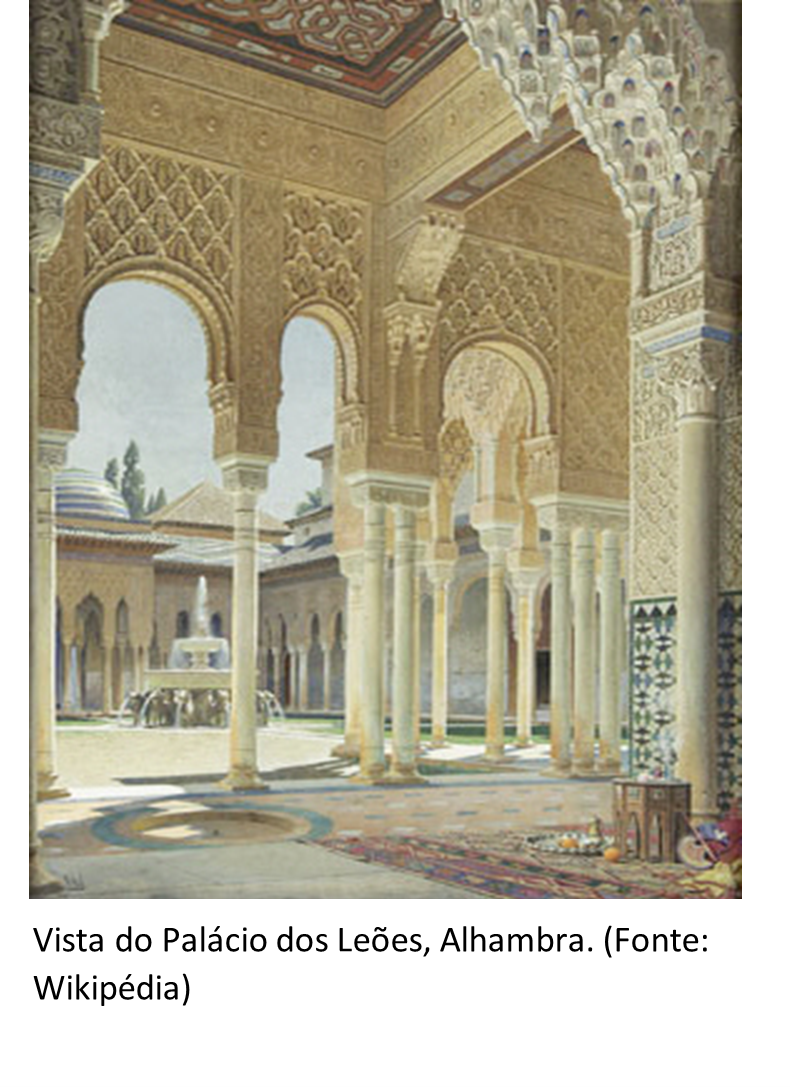
\includegraphics[width=.4\linewidth]{transformacoes9}
\end{figure}

Na figura a seguir, você encontra um padrão similar àqueles dos mosaicos que adornam Alhambra: 


\begin{figure}[H]
\centering

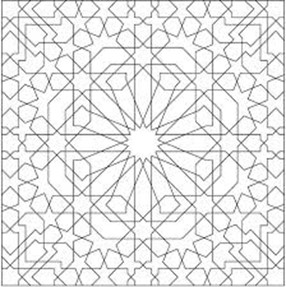
\includegraphics[width=.5\linewidth]{transformacoes10}
\end{figure}

\begin{enumerate}
\item No padrão geométrico exibido, encontre quatro pares de figuras congruentes. Entre um par e outro, tente selecionar figuras com diferentes formatos! Você pode pintar as figuras de um mesmo par da mesma cor, usando a figura disponível no Anexo 2, ao final desta seção. 
\item Para cada par de figuras que você selecionou, descreva o(s) movimento(s) que permitiria(m) sobrepor uma à outra. 
\item Ainda, no Anexo 3, uma figura desse padrão geométrico está em destaque. Tente encontrar todas as figuras congruentes a ela e indique quais são os movimentos envolvidos em suas possíveis sobreposições. 
\end{enumerate}


\item Identifique, visualmente, na imagem a seguir, pelo menos dois pares de figuras congruentes. Então, descreva o movimento que permite sobrepor tais figuras

\begin{figure}[H]
\centering

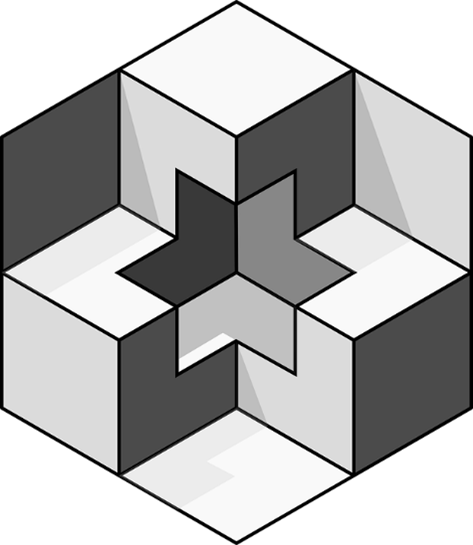
\includegraphics[width=.35\linewidth]{transformacoes11}
\end{figure}

\item Muitas vezes, encontrar figuras congruentes permite resolver de forma mais fácil e ágil alguns problemas geométricos que, de outra forma, teriam resolução longa ou complexa. Vamos ver?
\begin{enumerate}
\item \textit{(Fundamentos da Matemática Elementar, v. 9, 6ª edição, pág. 271-I, Exercício I.637 Adaptado)} Na figura a seguir, $O$ é ponto médio do segmento $DC$. Os segmentos $AM$, $MB$, $BC$ e $AD$ têm a mesma medida. Encontre a área hachurada, sabendo que o perímetro do retângulo $ABCD$ mede $42$ cm.  

\begin{figure}[H]
\centering

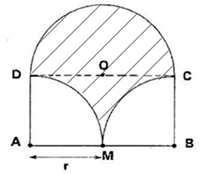
\includegraphics[width=.4\linewidth]{transformacoes12}
\end{figure} 

\item \textit{(Obmep Nível I - 2012, questão 6 )} O retângulo a seguir, que foi recortado de uma folha de papel quadriculado, mede 4 cm de largura por 5 cm de altura. 
 
\begin{figure}[H]
\centering

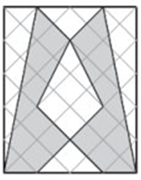
\includegraphics[width=.3\linewidth]{transformacoes13}
\end{figure}

Qual é a área da região cinzenta?
\begin{enumerate}
\item $10$ cm\super{2}. 
\item $11$ cm\super{2}.
\item $12{,}5$ cm\super{2}.
\item $13$ cm\super{2}.
\item $14{,}5$ cm\super{2}.
\end{enumerate}
\end{enumerate}
\end{enumerate}

\begin{paginatexto}{Seção 2 - Transformações isométricas: translações, rotações, reflexões}
\subsection{Objetivos Específicos}
\begin{itemize}
\item Identificar e descrever cada uma das transformações isométricas, usando recursos diversos (malhas e recursos tecnológicos diversos), em diferentes contextos.
\item Aplicar concretamente as transformações isométricas para construir figuras, em diversos contextos, utilizando diferentes tipos de recurso. 
\item Aplicar composições de isometrias para construir figuras, em diversos contextos, utilizando diferentes tipos de recurso. 
\end{itemize}

\textbf{Quantidade de aulas previstas para a seção}: 06 horas/aula.

\paragraph{Enriquecimento da discussão}
A proposta da seção é tratar o tema a fim de propiciar o avanço da compreensão dos alunos no estudo de isometrias de modo gradual, a fim de que eles desenvolvam familiaridade e traquejo nas situações que envolvem essas transformações.  A princípio, não são dadas definições de translações, rotações e reflexões; mesmo assim, nas partes “Explorando” são oferecidos exemplos em que é possível identificar as transformações presentes. Além disso, algumas perguntas devem estimular a turma a discutir, a desenhar e a fazer esquemas para representar as isometrias. Em particular, na apresentação de translações e rotações deve ficar clara a associação com movimentos naturais da realidade. Elas são apresentadas com ricos exemplos baseados na azulejaria; trata-se de um bom terreno para nos restringirmos às translações e rotações: movimentos realizados exclusivamente no plano. As reflexões em relação a retas até aparecem nessa primeira abordagem, mas são trabalhadas de fato, posteriormente nesta mesma seção, por meio de vários exemplos de mandalas.

\paragraph{Organização da turma}
Recomenda-se que os alunos trabalhem em duplas ou em pequenos grupos e que sejam estimulados a se expressarem sobre cada situação apresentada. A socialização dos resultados deve ser organizada pelo professor. Espera-se imprimir uma dinâmica de trabalho que favoreça o envolvimento e a participação de todos. 

\paragraph{Sobre as atividades da seção}
São atividades para pôr a mão na massa, a depender das habilidades dos alunos. As atividades de reconhecimento servem como um diagnóstico da familiaridade dos alunos com os temas apresentados; em muitas delas são fornecidos anexos e os alunos poderão, desenhar, recortar e manipular as figuras; nesses momentos eles devem ser orientados a utilizar régua, esquadros, compasso e, até mesmo, artefatos concretos como hastes, varetas, palitos discos e espelhos. A partir do reconhecimento de que duas figuras congruentes diferem pela aplicação de uma translação ou rotação, convidamos o aluno a descrever tal isometria. No caso em que duas figuras estão relacionadas por translação, a descrição natural do movimento será feita por meio de flechas que ligam os vértices homólogos das figuras congruentes. No caso em que as figuras estão relacionadas por uma rotação, a descrição do movimento é feita por meio de arcos de circunferência, com centro em um ponto indicado, que ligam vértices homólogos.  

Há também atividades em que os alunos serão convidados a analisar que transformação teria sido aplicada para levar uma figura a uma nova posição ou construir a imagem de uma figura dada por aplicação de uma isometria.

\paragraph{Dificuldades}
As dificuldades costumam aparecer quando as translações ou o eixo de reflexão são oblíquos. 

Também é comum que apareçam dificuldade de reconhecer, descrever e construir figuras congruentes nos casos em que a figura original e sua imagem têm interseção.

Outra dificuldade usual é descobrir o centro de rotação, assim como identificar rotação quando o centro está fora da figura.

\end{paginatexto}

\explore{Translações e rotações}

Você conhece o artista brasileiro Athos Bulcão?

Nascido no Catete, Rio de Janeiro, em 2 de julho de 1918, Athos foi um pintor, escultor e desenhista. Sua obra foi associada, no Brasil e no exterior, aos mosaicos em azulejo que produziu a partir da década de 1940, quando abandonou o curso de medicina para se dedicar à pintura. Nessa época, tornou-se assistente de Candido Portinari na construção do painel de São Francisco de Assis, na Igreja da Pampulha, em Belo Horizonte, marco da arquitetura moderna brasileira.

\begin{figure}[H]
\centering
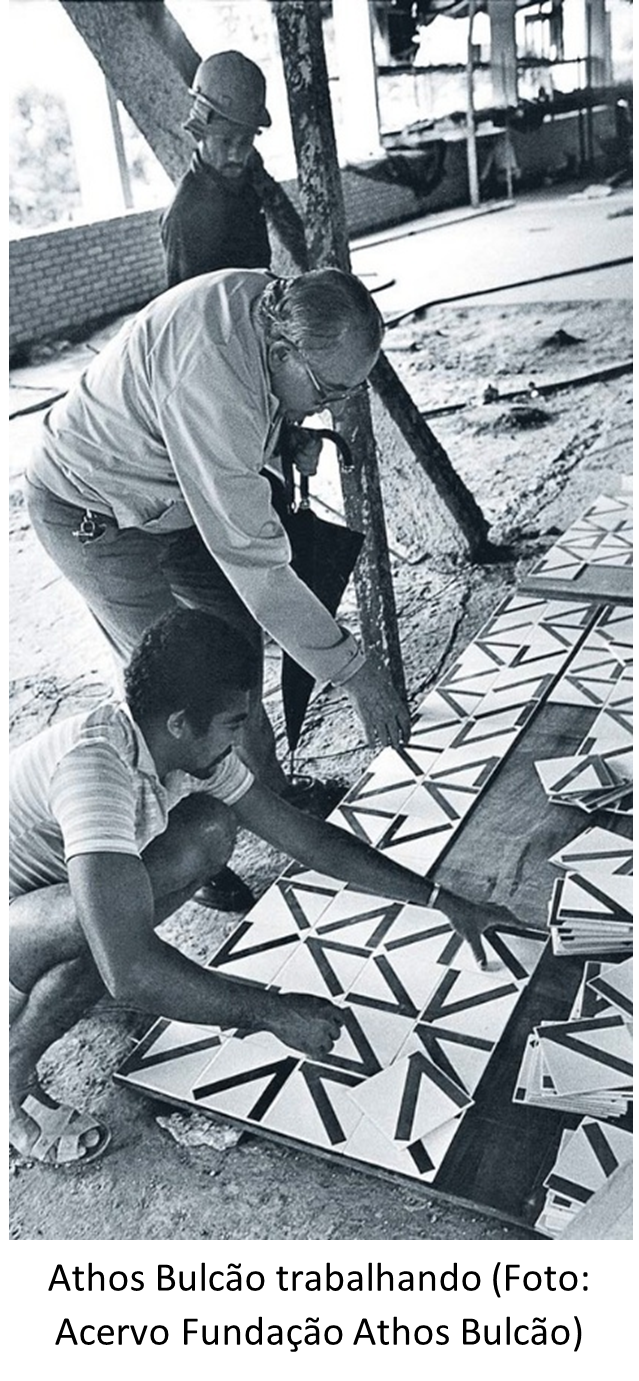
\includegraphics[width=.24\linewidth]{transformacoes14}
\end{figure}

A azulejaria praticada por Athos Bulcão mescla a repetição de padrões e a aleatoriedade, criando um efeito de movimento e liberdade que lhe rendeu um lugar de destaque na arte brasileira do século XX. 

O artista viveu em Brasília de 1958 até 2008 (ano de sua morte), contribuindo para fazer dessa cidade um museu a céu aberto. 

\begin{figure}[H]
\centering

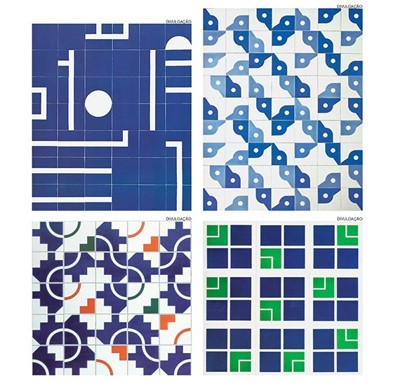
\includegraphics[width=.35\linewidth]{transformacoes15}
\caption{Reproduções de padrões de azulejos criados por Athos Bulcão (Foto: Divulgação)}
\end{figure}

Analisando a obra de azulejaria de Athos Bulcão, podemos observar que os azulejos de um mesmo tipo – que apresentam formas congruentes - se relacionam usualmente por \textbf{translações} e \textbf{rotações}. Observe os azulejos em destaque: 

\begin{figure}[H]
\centering

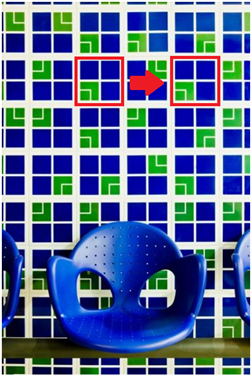
\includegraphics[width=.425\linewidth]{transformacoes16}
\hspace{2em}
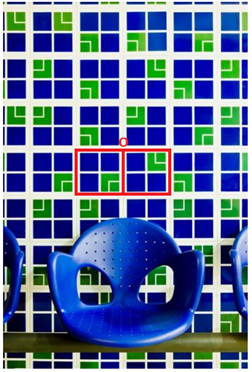
\includegraphics[width=.425\linewidth]{transformacoes17}
\caption{Hospital das Forças Armadas INCOR, Brasília. (Foto: Edgard Cesar)}

\end{figure}

No primeiro par de azulejos em destaque, a sobreposição entre os azulejos pode ser feita por meio de uma translação horizontal, deslocando o da esquerda duas “unidades” para a direita. (Note que estamos considerando o lado do azulejo quadrado como unidade.) No segundo par de azulejos em destaque, eles podem ser sobrepostos rotacionando $90^{\circ}$ o azulejo da esquerda, no sentido anti-horário, em torno do ponto $O$.  (Ver destaque a seguir.)

\begin{figure}[H]
\centering

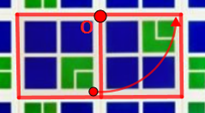
\includegraphics[width=.35\linewidth]{transformacoes18}
\end{figure}

\begin{knowledge}
Você pode conhecer mais sobre o artista e sua obra em: 
\url{https://www.fundathos.org.br/}

\end{knowledge}
\clearpage

\marginpar{\vspace{-1.25em}}
\begin{objectives}{Translações e rotações na azulejaria de Athos Bulcão}
{
O objetivo específico a atingir aqui é o de identificar e descrever movimentos rígidos no plano. Em todos os itens o aluno é convidado a identificar e descrever translações ou rotações nas situações indicadas. A princípio, os alunos podem ficar livres para decidir qual é a posição inicial e qual a posição final da figura, mas, para facilitar o diálogo, pode ser combinado previamente com a turma, em cada destaque, que peça será movida (posição inicial) e qual será a posição final. Recomenda-se que o professor comece a usar os termos: figura transladada e figura rotacionada. Nos itens c e d, os alunos são convidados a aplicar rotações a uma figura e podem ser estimulados a prever resultados. 
}{1}{1}
\end{objectives}
\begin{sugestions}{Translações e rotações na azulejaria de Athos Bulcão}
{
\textbf{Material necessário}: Uma folha contendo o anexo 5, por dupla, nos itens \titem{a)} e \titem{b)}, e uma folha contendo o anexo 6 no item \titem{c)}.
\begin{enumerate}[label=\titem{\alph*)}]
\item A atividade pode ser realizada por duplas de alunos. Em primeiro lugar o professor deve estimulá-los a reconhecer o deslocamento ocorrido em cada caso (translação nos destaques 1 e 2 e rotação nos destaques 3 e 4). Se for necessário, um azulejo recortado do anexo 5 pode auxiliar a reconhecer o movimento que permite sobrepor uma peça do par à outra. Espera-se que os alunos identifiquem uma malha quadriculada no painel e a utilizem para descrever oralmente os movimentos contando casas para a direita ou esquerda, para cima ou para baixo no caso das translações. Por exemplo, “duas casas na vertical para baixo (ou para cima, conforme a referência)” no destaque 1 e “uma casa para a direita e duas para baixo” no destaque 2. Já para a descrição das translações nos destaques 1 e 2, espera-se que os alunos, com sugestão do professor se necessário, liguem os vértices homólogos dos quadrados; aqui há que levar em conta que é a observação da mudança de posição do desenho dentro do azulejo que permite estabelecer a correspondência entre vértices homólogos. A atividade pode ser bem explorada: os alunos podem ser levados a   observar que o comprimento, direção e sentido dos segmentos orientados não se alteram nas translações. Para os destaques 3 e 4, o professor pode, por meio de sugestão de algumas tentativas, levar a turma a perceber que não há movimento de translação que relacione as figuras do par. Em seguida, se houver necessidade, pode sugerir que o azulejo recortado seja pregado em uma haste (um palito ou um lápis) que com a ponta oposta fixada no ponto P, no destaque 3, seja girada até encontrar a figura final. No destaque 4, o aluno deve fixar a haste no vértice R do quadrado inicial e explorar as possibilidades de rotação até encontrar a figura final. 
\end{enumerate}
}{1}{1}
\end{sugestions}
\begin{sugestions}{Translações e rotações na azulejaria de Athos Bulcão}
{
\begin{enumerate}[label=\titem{\alph*)}]\setcounter{enumi}{1}
\item As duplas de alunos devem ser estimuladas a descobrirem e descreverem translações e rotações que levam um azulejo do painel em outro. Depois as duplas podem expor suas escolhas para a turma toda.
\item Se houver necessidade os alunos podem colocar uma tachinha no centro do quadrado ou simplesmente imaginar que há um pino ali.
\item Já é hora de abstrair e os alunos podem ser levados a observar a figura estampada no azulejo e comparar com o que ocorreu no item anterior.
\end{enumerate}
}{1}{2}
\end{sugestions}
\begin{answer}{Translações e rotações na azulejaria de Athos Bulcão}
{
\begin{enumerate}
\item Destaque 1: movimento de translação. Três casas na vertical para baixo (ou para cima, conforme a referência). 

Destaque 2: movimento de translação (oblíqua) que corresponde a deslocar o azulejo uma casa para a direita e três casas para baixo (a ordem desses movimentos depende do que foi estabelecido na turma). Nos dois casos o movimento pode ser identificado de maneira concreta apoiando a figura original sobre uma régua; além disso as translações podem ser indicadas por meio de flechas -- segmentos orientados -- que associam os vértices da figura inicial aos seus correspondentes na figura final. 

Destaque 3: a figura do lado esquerdo foi girada de um ângulo de $90^{\circ}$ em torno do ponto $P$ em sentido horário (ou a da direita foi girada de $90^{\circ}$ em sentido anti-horário). 

Destaque 4: a figura do lado esquerdo foi girada de um ângulo de $90^{\circ}$ em torno do ponto $P$ em sentido horário (ou a da direita foi girada de $90^{\circ}$ em sentido anti-horário). Nos dois casos, as rotações podem ser indicadas por meio de arcos (inclusive orientados) que ligam um ponto da figura inicial ao ponto homólogo da figura final.

\item Há muitas possibilidades.

\item \adjustbox{valign=t}
{
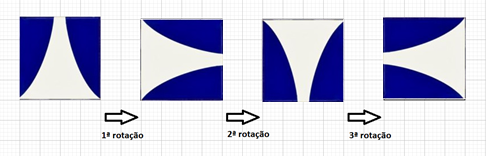
\includegraphics[width=.95\linewidth]{transformacoes26}
}

\item Não. A figura no azulejo não se altera por rotações de $90^{\circ}$.  
\end{enumerate}
}{1}
\end{answer}

\begin{sugestions}{Mosaico tipo Escher com translações ou }
{
A obra de M.C. Escher é fonte riquíssima para explorar as transformações geométricas. O item \titem{a)} tem a função de apresentar a obra do artista para os alunos.  Os efeitos visuais dos mosaicos de Escher costumam impressionar os estudantes, que tendem a ficar bastante motivados ao observar que fazer um mosaico inspirado na obra do artista é algo acessível a partir dos conhecimentos geométricos que estão estudando. 

Os itens \titem{a)} até \titem{d)}, podem ser realizados em casa. Então, em aula, após breve discussão sobre a pesquisa e sobre os vídeos, o item e deve ser discutido em profundidade. O professor deve ajudar os alunos a formular a diferença dos dois procedimentos construtivos da figura que forma o mosaico, mostrando que um deles está relacionado a rotações e outro a translações. Pode ser necessário ter os vídeos disponíveis para serem assistidos em aula.

A partir dessa discussão, o item \titem{f)} pode ser proposto como um pequeno projeto, com um intervalo de tempo suficiente para que os alunos possam tirar qualquer dúvida que surja no processo. É importante atentar para um possível resultado inesperado: os alunos podem inverter involuntariamente o a face do molde que fica para cima ou para baixo ao usá-lo para desenhar o mosaico. Isso afetará o padrão produzido, que deixará de ser apenas de rotação ou de translação. (A reflexão pode acabar sendo incluída ou, então, o aluno pode acabar se perdendo ao usar, sem perceber, dois tipos de transformação.) Para evitar isso, é possível sugerir que eles trabalhem com papel cartão, que costuma ter uma face colorida e outra crua. Mas, caso aconteça, o professor pode chamar a atenção dos alunos para o fato de ser possível identificar que isso aconteceu apenas olhando o resultado.

Organizar uma exposição com os mosaicos criados pelos estudantes pode ser excelente incentivo. 
Vídeo extra para o professor: \url{https://www.youtube.com/watch?v=Vm4zLz1DtkM}
}{1}{1}
\end{sugestions}



\begin{task}{Translações e rotações na azulejaria de Athos Bulcão}
\begin{enumerate}
\item Na fotografia a seguir você encontra o painel “Parada de descanso” (1985), de Athos Bulcão, que está no Parque da Cidade, em Brasília.  

\begin{figure}[H]
\centering

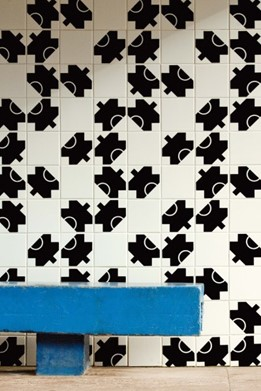
\includegraphics[width=.3\linewidth]{transformacoes19}
\end{figure}

Em cada caso, reconheça se pode ser utilizada uma translação ou uma rotação para sobrepor os azulejos destacados em vermelho. Se pode ser utilizada uma translação, descreva-a por meio de palavras e também desenhando, no Anexo 5, flechas que ligam pontos correspondentes. Se puder ser usada uma rotação, descreva-a por meio de palavras e também desenhando, no Anexo 5, arcos, com centro apropriado, para ligar pontos correspondentes. 

\begin{multicols}{2}
\begin{itemize}
\item Destaque 1
\begin{figure}[H]
\centering

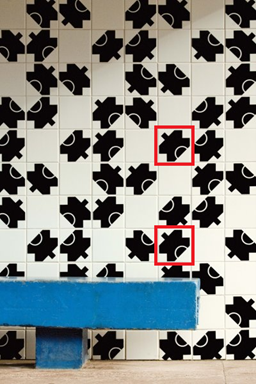
\includegraphics[width=.6\linewidth]{transformacoes20}
\end{figure}

\item Destaque 2
\begin{figure}[H]
\centering

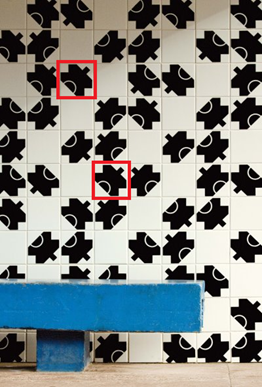
\includegraphics[width=.6\linewidth]{transformacoes21}
\end{figure}
\end{itemize}
\end{multicols}

\begin{multicols}{2}
\begin{itemize}
\item Destaque 3 (Dica: use o ponto P como referência!)
\begin{figure}[H]
\centering

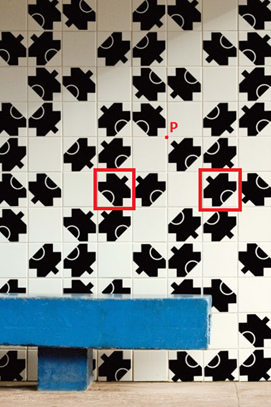
\includegraphics[width=.6\linewidth]{transformacoes22}
\end{figure}

\item Destaque 4 (use o ponto R como referência)
\begin{figure}[H]
\centering

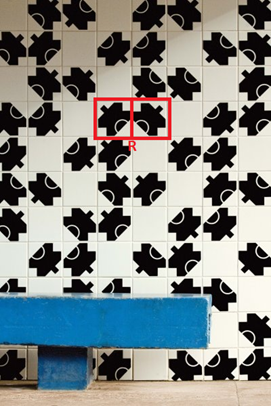
\includegraphics[width=.6\linewidth]{transformacoes23}
\end{figure}
\end{itemize}
\end{multicols}

\item Agora, no mesmo painel “Parada de Descanso”, escolha um par de azulejos e descreva a translação ou a rotação que permite sobrepor um ao outro. Use o Anexo 5 para desenhar. 


\item Agora, você vai usar um raciocínio diferente. Em vez de comparar rotações de azulejos em um painel já montado, como proposto anteriormente, você vai desenhar rotações sucessivas do azulejo quadrado dado na figura. Você deverá aplicar três rotações de 90° no sentido horário, em torno de seu ponto central, desenhando-nas nos quadrados em branco. Use o Anexo 6 para desenhar os azulejos rotacionados. A malha quadriculada será útil nesse processo.

\begin{figure}[H]
\centering

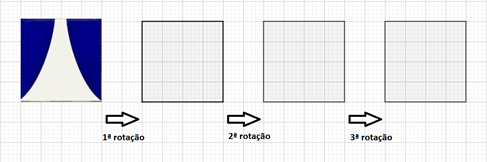
\includegraphics[width=.7\linewidth]{transformacoes24}
\end{figure}

\item Se você fizer o mesmo que no item anterior com este outro azulejo, o efeito será o mesmo? Comente.

\begin{figure}[H]
\centering

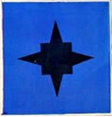
\includegraphics[width=.2\linewidth]{transformacoes25}
\end{figure}
\end{enumerate}

\end{task}

\begin{task}{Mosaico tipo Escher com translações ou rotações}
\begin{enumerate}
\item Outro artista que se valeu da Geometria para criar mosaicos fantásticos foi o holandês M.C. Escher (1898 – 1972). Caso não conheça, faça uma rápida busca na internet pelos mosaicos criados por esse artista.

\item Você também pode fazer um mosaico inspirado no trabalho de M. C. Escher de uma forma bastante simples. Veja o vídeo a seguir: \url{https://www.youtube.com/watch?v=Ca5J_moee7U}

\item No mosaico criado pelo processo descrito no vídeo, duas figuras adjacentes se relacionam por meio de translações ou rotações?

\item Agora, assista a essa sequência de vídeos: 
\begin{itemize}
\item Parte 1: \url{https://www.youtube.com/watch?v=TLWy3TZ-91o}
\item Parte 2: \url{https://www.youtube.com/watch?v=UBW5frsWiSI}
\item Parte 3: \url{https://www.youtube.com/watch?v=2IyOxI87GvY}
\end{itemize}

\item Nessa última sequência de vídeos, ao criar a figura base para o mosaico, qual foi a diferença essencial com relação ao processo mostrado no primeiro vídeo? Como essa diferença afeta o produto final?

\item Crie seu próprio mosaico usando um dos processos apresentados. Você vai precisar de um papel de boa gramatura, de fita adesiva e material para desenhar e colorir. Mãos à obra!
\end{enumerate}
\end{task}

\arrange{Translações e rotações}

Vimos que dois azulejos idênticos presentes em um painel criado por Athos Bulcão puderam ser sobrepostos por meio de \textbf{translações} ou \textbf{rotações} que, assim como as reflexões em relação a uma reta (que veremos mais adiante), são \textbf{isometrias}. 

A palavra isometria vem do grego e significa \textit{mesma medida}. Intuitivamente, podemos entender as isometrias como \textbf{movimentos rígidos}, isto é, que não deformam, não ampliam e nem diminuem as figuras geométricas sobre as quais são aplicadas, apenas modificam sua posição no plano. Em outras palavras, as isometrias preservam as distâncias entre os pontos das figuras. Por exemplo, tomemos os pentágonos congruentes $ABCDE$ e $A'B'C'D'E'$, mostrados na \fref{transformacoes27}, que se relacionam por meio de uma translação. Tomando quaisquer dois pontos $P$ e $Q$, na região interior ao primeiro pentágono, e seus correspondentes $P'$ e $Q'$, na região interior ao segundo pentágono, teremos que a distância entre $P$ e $Q$ é igual à distância entre $P'$ e $Q'$. Em linguagem matemática, dizemos que $d(P,Q) = d(P',Q')$.

\begin{figure}[H]
\centering

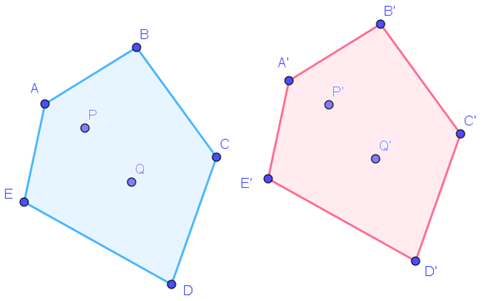
\includegraphics[width=.675\linewidth]{transformacoes27}
\caption{}
\label{transformacoes27}
\end{figure}

A preservação da distância entre pontos tem uma série de implicações, tais como a preservação das medidas dos ângulos e das medidas de área, por exemplo. 

\subsection{Translações}

Na atividade 1 do “Explorando”, você indicou \textbf{translações}, nos destaques 1 e 2, ligando cada vértice de um azulejo por meio de uma flecha – segmento orientado – ao seu correspondente na figura final ou figura transladada. Observe que todos os segmentos desenhados no destaque abaixo, por exemplo, têm mesma direção, mesmo sentido e mesmo comprimento.  Dizemos que essas flechas (\fref{transformacoes28}) representam um mesmo \textbf{vetor}

\begin{figure}[H]
\centering

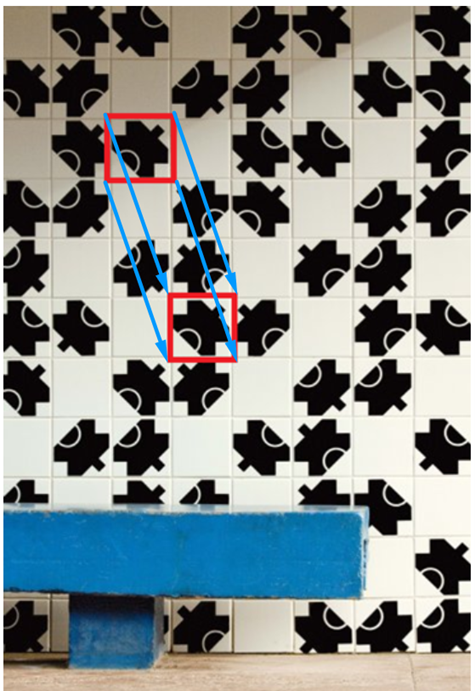
\includegraphics[width=.5\linewidth]{transformacoes28}
\caption{}
\label{transformacoes28}
\end{figure}

A ideia mais intuitiva que podemos usar para compreender o que é um vetor é a de uma “flecha” (por isso, para designá-los, usamos uma notação em forma de flecha). Só que um vetor tem direção, sentido e comprimento fixos, mas seu “ponto inicial” pode ser colocado em qualquer lugar do plano, dando origem a vários representantes diferentes. Observe os exemplos na \fref{transformacoes29}.

\begin{figure}[H]
\centering

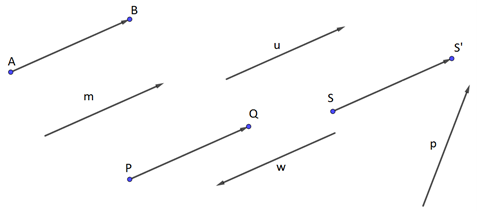
\includegraphics[width=.9\linewidth]{transformacoes29}
\caption{}
\label{transformacoes29}
\end{figure}

Na figura, podemos considerar que $\overrightarrow{AB}$, $\overrightarrow{m}$, $\overrightarrow{u}$, $\overrightarrow{PQ}$ e $\overrightarrow{SS'}$ são diferentes representações do mesmo vetor, pois têm mesma direção, sentido e comprimento. Mas $\overrightarrow{w}$ é um vetor diferente, pois tem mesmo comprimento e mesma direção de $\overrightarrow{AB}$, mas sentido oposto. (Dizemos que $\overrightarrow{AB}$ e $\overrightarrow{w}$ são vetores opostos.) Já $\overrightarrow{p}$ tem apenas o mesmo comprimento de $\overrightarrow{AB}$, mas sua direção é diferente. 

\begin{knowledge}
O conceito de vetor é importantíssimo não apenas na Matemática, mas também na Física, em que as grandezas que apresentam direção e sentido são, inclusive, chamadas de \textit{grandezas vetoriais}. 

O Livro Aberto de Matemática tem um capítulo dedicado exclusivamente ao estudo dos vetores. Assim, para aprofundar seu entendimento sobre o assunto, acesse-o!
\end{knowledge}

Uma translação relaciona-se à ideia de um movimento retilíneo, que fica determinado por sua \textit{direção}, \textit{seu sentido} e \textit{seu comprimento}. Por isso, podemos usar vetores para identificar (e descrever) as translações. 

Se tomarmos duas figuras congruentes que se relacionam por uma translação, então pares de pontos correspondentes determinarão sempre o mesmo vetor (ou seu oposto, a depender da orientação do segmento que os têm por extremidade). No painel da \fref{transformacoes30}, por exemplo, os pontos correspondentes das figuras contidas em dois dos azulejos determinam o mesmo vetor $\overrightarrow{v}$. Nesse caso, podemos dizer que uma das figuras (a que está mais abaixo, à direita) é a imagem da outra por uma translação de vetor $\overrightarrow{v}$.

\begin{figure}[H]
\centering

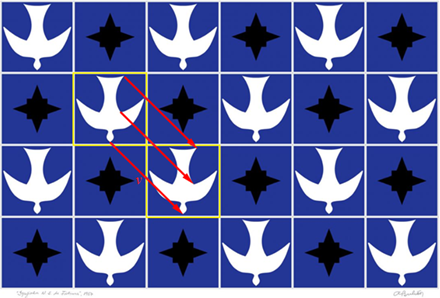
\includegraphics[width=.8\linewidth]{transformacoes30}
\caption{Igrejinha de N. S. de Fátima, Athos Bulcão, 1957}
\label{transformacoes30}
\end{figure}

\subsection{Rotações}


Uma rotação, por sua vez, relaciona-se à ideia de um movimento circular. Na Atividade 1 do “Explorando”, nos destaques 3 e 4, vimos exemplos de rotações. Para representar a rotação que ocorre em um deles, podemos ligar pontos do azulejo inicial aos pontos correspondentes no azulejo final por meio de arcos, com centro no ponto $O$, como na \fref{transformacoes31}Figura 5. É importante destacar que, se a rotação leva um ponto A em um ponto $A'$ então o comprimento do segmento $OA$ é igual ao comprimento do segmento $OA'$.

\begin{figure}[H]
\centering

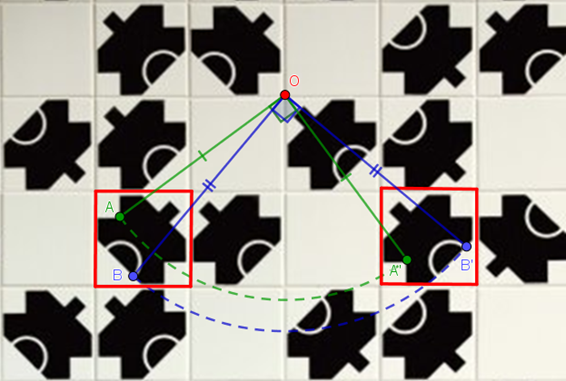
\includegraphics[width=.8\linewidth]{transformacoes31}
\caption{}
\label{transformacoes31}
\end{figure}

Uma rotação fica determinada, portanto, por um centro, por um ângulo “de giro” e por um sentido, que pode ser horário ou anti-horário.  Por simplicidade de linguagem, podemos adotar a ideia de \textbf{ângulo orientado}, com sinal positivo para o sentido anti-horário e com sinal negativo para o sentido horário, como se vê na \fref{transformacoes32}. 


\begin{figure}[H]
\centering

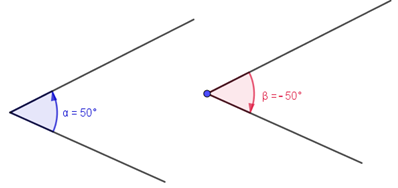
\includegraphics[width=.8\linewidth]{transformacoes32}
\caption{}
\label{transformacoes32}
\end{figure}

Dado um ponto $P$ qualquer em uma figura plana, sobre a qual é aplicada uma rotação de centro $O$ (distinto de $P$) e ângulo $\theta$, o correspondente de P por essa rotação será o ponto P’ pertencente à circunferência de centro $O$ e raio $\overline{OP}$, de tal modo que o ângulo orientado $POP'$ seja igual a $\theta$. 
Veja o exemplo a seguir (\fref{transformacoes33}), em que o quadrado $KLMN$ é rotacionado de $45^{\circ}$ em torno do ponto $O$. O resultado é o quadrado $K'L'M'N'$. Observe que $K$ e $K'$, por exemplo, pertencem à mesma circunferência de centro $O$ e raio $\overline{OK}$, sendo que o ângulo orientado $KOK'$ mede $45^{\circ}$. O mesmo acontece com qualquer par de pontos homólogos; $M$ e $M'$ pertencem à circunferência de centro $O$ e raio $\overline{OM}$ (observe que esse segmento é diferente de $\overline{OK}$) e o ângulo orientado $MOM'$ também mede $45^{\circ}$.

\begin{figure}[H]
\centering

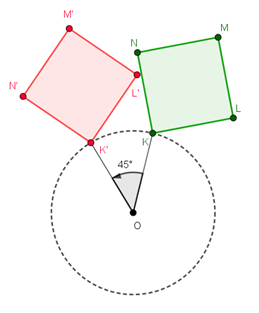
\includegraphics[width=.4\linewidth]{transformacoes33}
\caption{}
\label{transformacoes33}
\end{figure}


Veja outro exemplo na \fref{transformacoes34}, baseado em um painel de Athos Bulcão. O azulejo do canto inferior direito pode ser visto como uma rotação de centro C e ângulo $-270^{\circ}$ do azulejo do canto superior direito.


\begin{figure}[H]
\centering

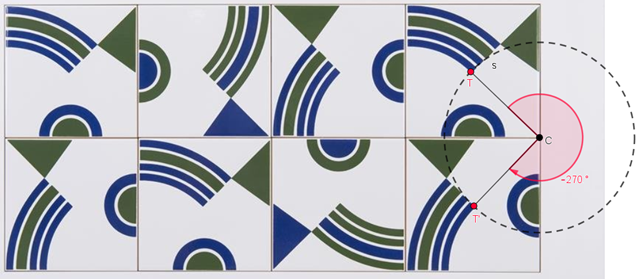
\includegraphics[width=.725\linewidth]{transformacoes34}
\caption{}
\label{transformacoes34}
\end{figure}

Observe, nesse último exemplo, que o ponto C está sobre a figura original (é um de seus vértices). O centro, quando está sobre a figura em que a rotação é aplicada, é o único de seus pontos que fica fixo.

\clearpage
\def\currentcolor{cor1}
\marginpar{\vspace{-.5em}}
\begin{sugestions}{Exercícios}
{
Vários dos exercícios aqui propostas pedem ao aluno que identifique e descreva translações e /ou rotações e contemplam, portanto, o objetivo específico 1 desta seção. Nos exercícios 2, 7 e 8 os alunos são convidados a construir as imagens de figuras dadas por translações e rotações, o que contribui para atingir o objetivo específico 2. O exercício 10 trata da composição dessas isometrias e está relacionada ao objetivo específico 3, estabelecido no início da seção.   

\tcbsubtitle{Exercício 1}

Em cada item, o estudante deve indicar o vetor por meio de vértices homólogos dos polígonos congruentes. Alguns alunos, podem optar por desenhar representantes do vetor que define cada translação. Descrições diferentes podem estar igualmente corretas, mas é importante esclarecer aos alunos que a translação fica descrita por um único representante do vetor que a define. 

Alguma dificuldade pode surgir no item \titem{c)}, em que a figura transladada contém partes da figura original.
Chame a atenção dos alunos para o fato de que o vetor que define a translação do item \titem{d)} é oposto ao do item \titem{a)}. Na verdade, a translação do item \titem{d)} é a operação inversa da translação do item \titem{a)}. 

\tcbsubtitle{Exercício 2}

Aqui temos um setor circular e os estudantes devem observar que o formato do arco de circunferência fica mantido por translações. Estimule os alunos a marcarem o ponto homólogo do centro do setor e os homólogos de suas extremidades, isto é, dos pontos $A$ e $B$; em seguida, os alunos devem usar compasso para desenhar os arcos das figuras transladas.  A translação pelo vetor $\overrightarrow{w}$  decerto não gerará dúvidas, mas a translação pelo vetor  $\overrightarrow{v}$  pode apresentar mais dificuldade, por se tratar de vetor oblíquo e porque a figura transladada ocupará partes do plano já ocupadas pela figura original.  
\tcbsubtitle{Exercício 3}

Recomenda-se voltar à questão 1 com a turma para comparar com o que aconteceu nos itens \titem{a)} e \titem{d)}. Isso dará ideia de que o vetor que define a translação é o vetor oposto àquele que define a translação inversa. 
}{1}{1}
\end{sugestions}
\begin{answer}{Exercícios}
{\exerciselist
\begin{enumerate}
\item 
\begin{enumerate}
\item Possibilidade: $\overrightarrow{QQ'}$
\item Possibilidade: $\overrightarrow{QQ''}$
\item Possibilidade: $\overrightarrow{Q''Q}$
\item Possibilidade: $\overrightarrow{Q'Q'}$
\end{enumerate}
\end{enumerate}
}{1}
\end{answer}
\marginpar{\vspace{-.75em}}
\begin{answer}{Exercícios p. \pageref{transformacoes-exercise2}}
{\exerciselist
\begin{enumerate}\setcounter{enumi}{1}
\item \adjustbox{valign=t}
{
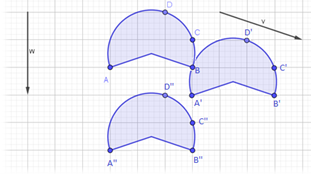
\includegraphics[width=.7\linewidth]{transformacoes43}
}
\item Pelo vetor oposto $\overrightarrow{QP}$
\end{enumerate}
}{0}
\end{answer}
\begin{sugestions}{Exercício 4}
{
Recomenda-se chamar a atenção dos alunos para as posições dos pontos $B$ e $B'$ na malha quadriculada. A partir do traçado dos raios $PB$ e $PB'$ fica claro que a rotação é de $90^{\circ}$ em sentido horário, ou seja, o ângulo de rotação é $-90^{\circ}$.

\tcbsubtitle{Exercício 5}

Aqui é interessante relembrar ou introduzir a noção de que o centro de uma circunferência pertence à mediatriz do segmento dado por dois pontos quaisquer sobre ela. Assim o centro será encontrado na interseção de mediatrizes de segmentos formados por pontos homólogos.
}{1}{2}
\end{sugestions}
\begin{answer}{Exercícios}
{\exerciselist
\begin{enumerate}\setcounter{enumi}{3}
\item $\hat{BPB'}$, que mede $90^{\circ}$

\item \adjustbox{valign=t}
{
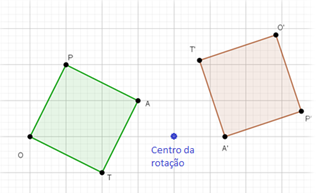
\includegraphics[width=.8\linewidth]{transformacoes44}
}
\end{enumerate}
}{1}
\end{answer}
\clearmargin
\begin{sugestions}{Exercício 6}
{
Uma rotação de 180° em torno do ponto médio do lado comum aos azulejos do par leva um azulejo no outro

\tcbsubtitle{Exercício 7}

A rotação de 90° em sentido horário do quadrado que emoldura a figura não deve apresentar dificuldade. No entanto, recomenda-se chamar a atenção dos alunos para o fato de que a rotação da figura desenhada dentro do quadrado também vai sofrer rotação e resultar em uma figura congruente a ela. Eles devem ficar atentos para que a rotação mantém o paralelismo entre segmentos e os lados do quadrado, mantém ângulos e comprimentos.    
}{1}{1}
\end{sugestions}
\begin{answer}{Exercícios}
{\exerciselist
\begin{enumerate}\setcounter{enumi}{5}
\item Rotação de $180^{\circ}$ em tono do ponto médio do lado comum aos azulejos.

\item \adjustbox{valign=t}
{
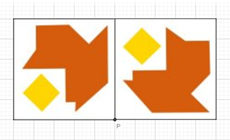
\includegraphics[width=.8\linewidth]{transformacoes45}
}
\end{enumerate}
}{1}
\end{answer}
\clearmargin
\begin{sugestions}{Exercício 8}
{
A figura obtida será congruente à figura original e, portanto, deve-se ter atenção para a manutenção dos ângulos (pode-se recomendar que comecem pelos ângulos retos) e dos comprimentos da figura original.

\tcbsubtitle{Exercício 9}
Recomenda-se levar os alunos a concluírem, informalmente, que uma figura rotacionada em sentido anti-horário deve ser rotacionada em sentido horário para voltar à posição original. Com mesmo centro e ângulo $-\alpha$. 

\tcbsubtitle{Exercício 10}
Metade da classe pode fazer primeiro a translação e depois a rotação e a outra metade pode fazer o contrário. 
}{1}{2}
\end{sugestions}
\begin{answer}{Exercícios}
{\exerciselist
\begin{enumerate}\setcounter{enumi}{7}
\item \adjustbox{valign=t}
{
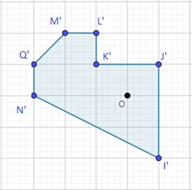
\includegraphics[width=.4\linewidth]{transformacoes46}
}

\item Rotação com o mesmo centro e ângulo $-\alpha$


\item Não são obtidas as mesmas imagens ao trocar a ordem da aplicação das isometrias citadas. 
\end{enumerate}

\begin{multicols}{2}
\centering
Rotação seguida de translação:

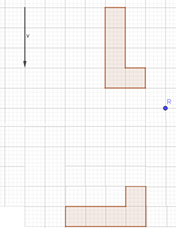
\includegraphics[height=5cm]{transformacoes47}

\columnbreak

Translação seguida de rotação:

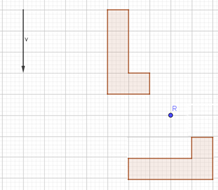
\includegraphics[height=5cm]{transformacoes48}
\end{multicols}
}{1}
\end{answer}

\exercise
\phantomsection\label{transformacoes-exercise2}

\begin{enumerate}
\item Considere o trio de polígonos congruentes. 

\begin{figure}[H]
\centering

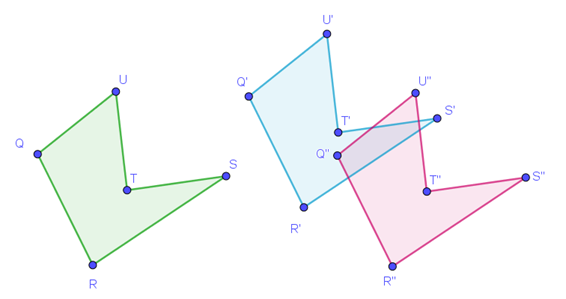
\includegraphics[width=.7\linewidth]{transformacoes35}
\end{figure}

Mencionando os vetores pertinentes, descreva a translação que leva
\begin{enumerate}
\item $QRSTU$ em $Q'R'S'T'U'$. 
\item $QRSTU$ em $Q''R''S''T''U''$.
\item $Q''R''S''T''U''$ em $Q'R'S'T'U'$.
\item $Q'R'S'T'U'$ em $QRSTU$.

\end{enumerate}

\item Utilize o Anexo 7 para desenhar o resultado da translação do setor circular por $\overrightarrow{w}$ e por $\overrightarrow{v}$.

\begin{figure}[H]
\centering

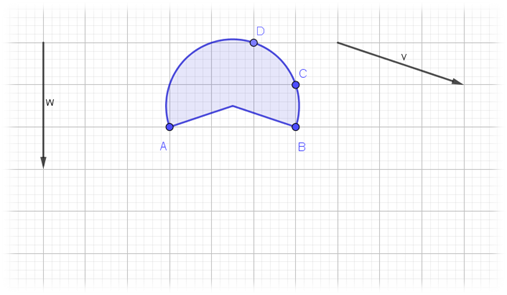
\includegraphics[width=.8\linewidth]{transformacoes36}
\end{figure}

\item Sabe-se que duas figuras congruentes $A$ e $B$ são tais que $B$ é a translação de $A$ pelo vetor $\overrightarrow{PQ}$. Nesse caso, $A$ é a translação de $B$ por qual vetor?

\item O triângulo $A'B'C'$ é resultado de uma rotação com centro em $P$ do triângulo $ABC$. Qual é o ângulo de rotação? Lembre-se de descrever o sentido da rotação ou de estabelecer um ângulo orientado, cujo sinal indica o sentido.

\begin{figure}[H]
\centering

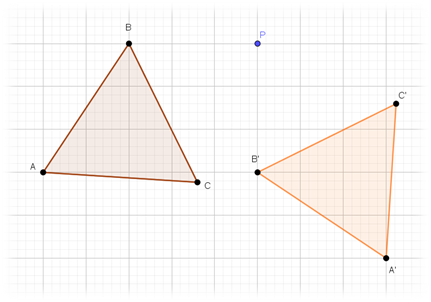
\includegraphics[width=.7\linewidth]{transformacoes37}
\end{figure}

\item Considere os quadrados $PATO$ e $P'A'T'O'$, que é sua imagem por uma rotação. Se $P$ e $P'$ são pontos correspondentes, bem como $A$ e $A'$, $T$ e $T'$, $O$ e $O'$, então você consegue descobrir o centro da rotação? Dica: lembre-se que um ponto e sua rotação então ambos na mesma circunferência... Então, se pergunte: dados dois pontos de uma mesma circunferência, o que você sabe sobre a localização do centro? Use o Anexo 8 para fazer construções com régua e compasso. Utilizar esses instrumentos é o melhor modo de descobrir o centro da rotação.

\begin{figure}[H]
\centering

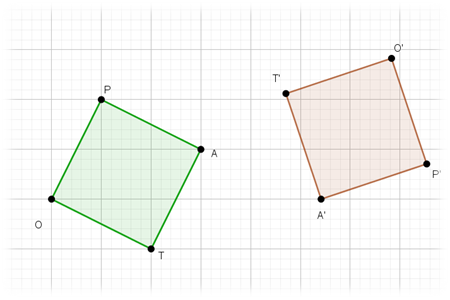
\includegraphics[width=.7\linewidth]{transformacoes38}
\end{figure}


\item Considere, mais uma vez, o painel “Parada de descanso” (1985), de Athos Bulcão, que está no Parque da Cidade, em Brasília. Descreva a rotação que permite sobrepor os dois azulejos destacados em vermelho. 

\begin{figure}[H]
\centering

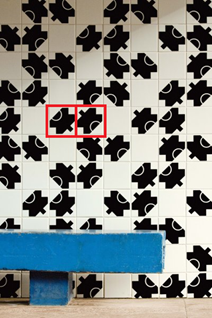
\includegraphics[width=.45\linewidth]{transformacoes39}
\end{figure}


\item Utilize o Anexo 9 para desenhar o resultado da rotação de centro $P$ e ângulo $-90^{\circ}$ aplicada sobre a figura dada. 

\begin{figure}[H]
\centering

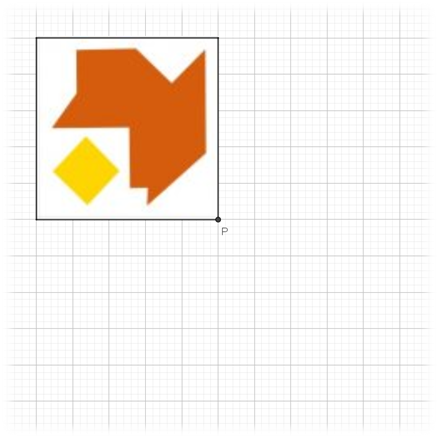
\includegraphics[width=.55\linewidth]{transformacoes40}
\end{figure}

\needspace{4em}

\item Utilize o Anexo 10 para desenhar o resultado da rotação de centro $O$ e ângulo $180^{\circ}$. 

\begin{figure}[H]
\centering

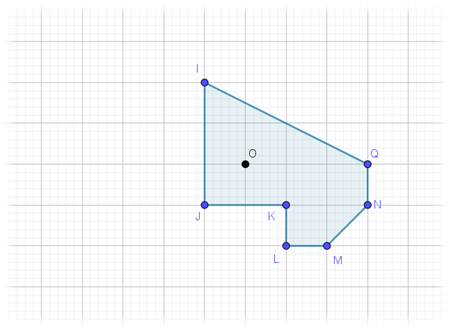
\includegraphics[width=.6\linewidth]{transformacoes41}
\end{figure}

\item Sabe-se que duas figuras congruentes $A$ e $B$ são tais que $B$ é a rotação de centro $O$ e ângulo $\alpha$ da figura $A$. Nesse caso, $A$ é a rotação da figura $B$ com qual centro e de qual ângulo?


\item Considere a rotação de centro $R$ e ângulo $90^{\circ}$ e a translação pelo vetor $\overrightarrow{v}$. Aline rotacionou o hexágono em forma de $L$, despois o transladou. Cláudia transladou esse mesmo hexágono, depois o rotacionou. Elas obtiveram o mesmo resultado? Justifique.

\begin{figure}[H]
\centering

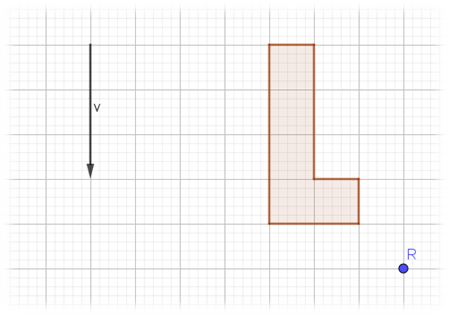
\includegraphics[width=.6\linewidth]{transformacoes42}
\end{figure}
\end{enumerate}


\explore{Reflexões em relação a uma reta}

Iniciamos este capítulo explorando o jogo eletrônico Tetris, que apresenta sete peças distintas, que, conforme vão “caindo” do alto da tela, devem ser movimentadas – com translações e rotações – de modo a se encaixarem perfeitamente nos espaços vazios deixados pelas peças anteriores, na parte de baixo da tela. 

\begin{figure}[H]
\centering

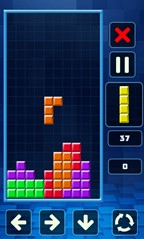
\includegraphics[width=.4\linewidth]{transformacoes1}
\caption{Tela do jogo Tetris}

\end{figure}

Dentre as sete pelas do jogo, há dois pares de figuras congruentes: as peças S e Z e as peças L e R. 

\begin{figure}[H]
\centering

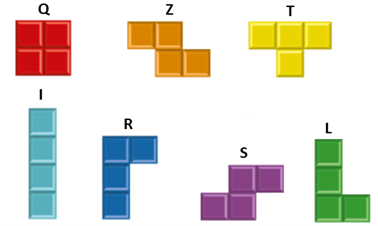
\includegraphics[width=.6\linewidth]{transformacoes2}
\caption{As sete peças do jogo Tetris}

\end{figure}

Embora S e Z sejam figuras congruentes, elas não se equivalem no jogo – ou seja, não são capazes de preencher os mesmos espaços. Isso acontece porque tais peças não podem ser sobrepostas usando translações ou rotações, os movimentos permitidos no jogo. Se fossem objetos físicos, não figuras geométricas abstratas, para sobrepor a peça S à peça Z do Tetris, teríamos de “retirá-la do plano”, virando-a no espaço, para só então colocá-la novamente sobre o plano, invertendo a face que fica visível. O mesmo vale em relação às peças R e L.

Figuras congruentes com essa propriedade – que não admitem sobreposição por rotações ou translações – são chamadas de figuras \textbf{enantimorfas}.  Para sobrepor figuras enantimorfas precisamos de um outro tipo de isometria, chamada \textbf{reflexão em relação a uma reta}. 
	
A ideia mais intuitiva que podemos ter acerca desse tipo de reflexão vem da nossa experiência com espelhos planos – “naturais”, como aqueles formados pelas águas tranquilas de um lago, ou os de vidro, feitos pelo homem, por exemplo. Em ambos os casos, são produzidas formas congruentes às originais, mas que, em geral, não poderiam ser sobrepostas por translações ou rotações. Em outras palavras, um espelho geralmente forma pares de figuras enantimorfas. 
	
Diversas formas de arte exploram intensamente as reflexões em relação a uma reta. Por exemplo, a fotografia de Joanna Lemanska, tirada na cidade de Nova York e apresentada na \fref{transformacoes49}, explora o efeito de um espelho d’água “acidental”, que duplica a paisagem urbana.

\begin{figure}[H]
\centering

\includegraphics[width=\linewidth]{transformacoes49}
\caption{Disponível em: \url{http://www.misscoolpics.com/photographs\#/6-days-in-new-york/}. Acesso em setembro de 2020}
\label{transformacoes49}
\end{figure}

Reflexões também podem relacionar pares de figuras que não são enantimorfas. Por exemplo, as figuras destacadas em verde, na mandala da \fref{transformacoes50}, podem ser sobrepostas por meio de uma rotação de $45^{\circ}$ em torno do ponto central da mandala.  Mas também podemos observar que uma dessas figuras é a reflexão da outra em relação à reta $r$.
\clearpage
\begin{objectives}{Reflexões em relação a uma reta}
{
As atividades deste bloco devem favorecer a familiarização dos alunos com as reflexões em relação a retas, identificando-as e descrevendo-as; ou seja, devem contemplar o objetivo específico 1 desta seção. 
}{1}{1}
\end{objectives}
\begin{sugestions}{Reflexões em relação a uma reta}
{
\begin{itemize}
\item Item \titem{a)}: Aqui os alunos devem separar as figuras em dois conjuntos distintos de modo que em cada um deles todos os pentágonos correspondam-se por movimentos rígidos do plano: translações, rotações ou compostas dessas isometrias. $A$ ideia principal é que duas figuras que estejam em conjuntos distintos são enantimorfas, ou seja não se correspondem por translações e rotações, mas somente por reflexões por uma reta. Pode-se orientar a turma a considerar a figura A e imaginar as possibilidades de translações e rotações que levem A às outras figuras em ordem alfabética. Logo, os alunos vão descobrir que o pentágono $E$ não está relacionado a $A$ por um desses movimentos, mas, sim, por meio de reflexão em relação a uma reta. 
\end{itemize}
}{1}{1}
\end{sugestions}
\begin{answer}{Reflexões em relação a uma reta}
{
\begin{enumerate}
\item Um conjunto é ${A, B, C, D, G}$ e o outro é ${E, F, H}$. 
\end{enumerate}
}{1}
\end{answer}
\clearmargin
\begin{sugestions}{Reflexões em relação a uma reta}
{
\begin{itemize}[wide]
\item Item \titem{c)}: Ao dobrar a folha fazendo com que os pontos $A$ e $B$ coincidam, o vinco corresponde ao eixo de reflexão dos dois pontos. Aqui pode-se orientar os alunos a traçarem o segmento AB, a reta onde fizeram a dobra e estimulá-los a descobrir o ângulo entre eles e medidas do segmento. Os alunos devem concluir que $AB$ é perpendicular ao eixo de reflexão e fica dividido ao meio por ele.  

\item Item \titem{d)}: Há várias possibilidades. Duplas de alunos podem escolher pares de figuras que se relacionam por reflexão e depois, em plenária, podem comparar as respostas. É interessante estimular a turma a procurar, na mandala, pares enantimorfos, ou seja, figuras que se relacionam por reflexão em relação à reta dada, mas não por translações ou rotações.

\item Item \titem{e)}: Esta atividade complementa a anterior e amplia a discussão sobre quais pares são relacionados por movimentos rígidos do plano e quais não são. A turma deve concluir que somente as figuras que são cortadas pela reta $r$ geram pares de figuras enantimorfas.  
\end{itemize}
}{1}{2}
\end{sugestions}
\begin{answer}{Reflexões em relação a uma reta}
{
\begin{enumerate}\setcounter{enumi}{1}
\item \adjustbox{valign=t}
{
\includegraphics[width=.95\linewidth]{transformacoes53}
}

\item O vinco é mediatriz do segmento AB.
\item Há várias possibilidades. 
\item Não.

\end{enumerate}
}{1}
\end{answer}
\clearmargin
\begin{sugestions}{Reflexões em relação a uma reta}
{
\begin{itemize}
\item Item \titem{f)}: Há várias possibilidades. Cada reta que liga o centro da mandala a qualquer ponta de uma estrela é eixo de reflexão de figuras enantimorfas. Os alunos devem representar a reflexão construindo o segmento que une um par de pontos correspondentes. Podem também verificar que a reta de reflexão é mediatriz desse segmento. 

\item Item \titem{g} Sugerimos ao professor que avalie se é o caso de remeter essa atividade para casa ou se, pelo contrário, ele próprio gostaria de projetar o vídeo para que todos assistam juntos. 

Como uma peça expressiva/artística, o vídeo pode ter múltiplas interpretações, mas, para aqueles que conhecem o conteúdo da série (muito popular entre 2019 e 2020), o uso das reflexões, produzindo imagens com padrões complexos, pode remeter à própria complexidade da trama, que lida com viagens no tempo e com a ideia de universos paralelos, que apresentam também algum tipo de “espelhamento”. 

Seja como for, o objetivo aqui é refletir sobre o uso expressivo das transformações.
\end{itemize}
}{1}{1}
\end{sugestions}
\begin{answer}{Reflexões em relação a uma reta}
{\begin{enumerate}\setcounter{enumi}{5}
\item Há várias possibilidades.
\end{enumerate}
}{1}
\end{answer}

\begin{figure}[H]
\centering

\includegraphics[width=.5\linewidth]{transformacoes50}
\caption{}
\label{transformacoes50}
\end{figure}

\begin{task}{Reflexões em relação a uma reta}

\begin{enumerate}
\item Todos os polígonos a seguir são congruentes. Separe-os em dois conjuntos, de modo que todo elemento de um deles faça um par de figuras enantimorfas com qualquer elemento do outro.  

\begin{figure}[H]
\centering

\includegraphics[width=.5\linewidth]{transformacoes51}
\end{figure}

\item Na fotografia de Joanna Lemanska, identifique e desenhe a reta de reflexão, isto é, a reta que “funciona como espelho” entre os objetos e suas imagens. Use o Anexo 11 para desenhar essa reta.

\begin{figure}[H]
\centering

\includegraphics[width=.8\linewidth]{transformacoes49}
\end{figure}

\item Pegue uma folha de papel e, sobre ela, marque dois pontos distintos quaisquer $A$ e $B$. Então, dobre a folha de modo a sobrepor os pontos $A$ e $B$. Usando a noção de reflexão em relação a uma reta, descreva a relação entre os pontos $A$ e $B$ e a reta representada pelo vinco.

\item Na mandala, selecione pelo menos mais três outros pares de figuras (que não cruzem a reta $r$) que podem ser relacionados por meio de uma reflexão em relação à reta $r$. Use o Anexo 12 para colorir os pares de figuras escolhidas.

\begin{figure}[H]
\centering

\includegraphics[width=.5\linewidth]{transformacoes50}
\end{figure}

\item Os pares de figuras que você selecionou no item anterior eram enantimorfos? Se não eram, indique rotações ou translações que permitiriam sobrepô-las.

\item Na mandala a seguir encontre um par de figuras enantimorfas e indique a reta de reflexão $r$. Marque pares de pontos $A$ e $A'$ que se correspondem pela reflexão e construa o segmento $AA'$. Verifique que $AA'$ é perpendicular à reta $r$ e fica dividido ao meio por ela. Use o Anexo 13 para fazer as construções necessárias.

\begin{figure}[H]
\centering

\includegraphics[width=.4\linewidth]{transformacoes52}
\end{figure}

\item Assista à abertura de uma das temporadas da série de suspense/ficção científica Dark, criada por Baran bo Odar e Jantje Friese. Depois, escreva um breve texto, descrevendo como as reflexões com relação a uma reta são utilizadas nessa abertura e qual é o efeito expressivo que ela produz. O vídeo está disponível aqui: \url{youtube.com/watch?v=Nu56ofHJgr0}. 
\end{enumerate}

\end{task}


\arrange{Reflexões em relação a uma reta}

As reflexões em relação a uma reta associam-se à noção intuitiva de espelhamento, podendo produzir pares de figuras enantimorfas (\fref{transformacoes54}) ou não (\fref{transformacoes55}). 

\begin{multicols}{2}
\begin{figure}[H]
\centering

\includegraphics[height=4cm]{transformacoes54}
\caption{}
\label{transformacoes54}
\end{figure}

\begin{figure}[H]
\centering

\includegraphics[height=4cm]{transformacoes55}
\caption{}
\label{transformacoes55}
\end{figure}
\end{multicols}
                      
Você já trabalhou com a mandala da \fref{transformacoes56} em uma atividade proposta anteriormente. Nela, o segmento AA’ liga pontos correspondentes dos triângulos destacados em vermelho. Esses triângulos se relacionam por uma reflexão em relação à reta r. O segmento AA’ é perpendicular a essa reta e fica dividido ao meio por ela. Isso sempre acontece e é a partir dessa propriedade que podemos escrever a definição a seguir. 

\begin{figure}[H]
\centering

\includegraphics[width=.4\linewidth]{transformacoes56}
\caption{}
\label{transformacoes56}
\end{figure}

Seja P um ponto qualquer em uma figura plana, sobre a qual é aplicada uma reflexão em relação a uma reta $m$, o correspondente de $P$ por essa reflexão será o ponto $P'$, de tal modo que a reta m seja a mediatriz de $\overline{PP'}$ (\fref{transformacoes57}). A única exceção vale para o caso de $P$ estar contido na reta $m$. Se for assim, então $P = P'$ (\fref{transformacoes58}).
 
\begin{multicols}{2}
\begin{figure}[H]
\centering

\includegraphics[height=3.75cm]{transformacoes57}
\caption{}
\label{transformacoes57}
\end{figure}

\begin{figure}[H]
\centering

\includegraphics[height=3.75cm]{transformacoes58}
\caption{}
\label{transformacoes58}
\end{figure}
\end{multicols}

A reta em relação à qual ocorre a reflexão é comumente chamada de eixo de reflexão.

\clearpage
\def\currentcolor{cor1}
\begin{objectives}{Exercícios}
{
Os exercícios 1 e 2 deste bloco são propostas de identificação e descrição de reflexões e, portanto, contribuem para alcançar o objetivo específico 1 da seção. No exercício 3, pede-se para aplicar reflexões e, na 4, compostas delas para construir figuras refletidas; elas contribuem para atingir os objetivos específicos 2 e 3, respectivamente.   
}{1}{1}
\end{objectives}
\begin{sugestions}{Exercício 1}
{
Somente em $A$ e $B$ é possível reconhecer reflexão. Esta é uma questão de reconhecimento visual e não se trata de determinar o eixo de reflexão. Em $C$, as figuras associam-se por translação; em $D$, por translação seguida de rotação. 

\tcbsubtitle{Exercício 2}

Os alunos deverão lembrar que, conforme a definição de reflexão em relação a uma reta, o eixo de reflexão é mediatriz do segmento formado por um par de vértices homólogos. Assim sendo, após reconhecer visualmente que as figuras estão associadas por reflexão e identificar os pares de vértices homólogos,  basta traçar o segmento que os une e, em seguida sua mediatriz $r$; verifica-se que $r$ é mediatriz do segmento que une outros dois pontos correspondentes quaisquer e, portanto, ela é o eixo de reflexão. Os itens $b$ e $c$ podem apresentar dificuldades, pois o item b tem um ponto fixo sobre o eixo de reflexão $e$, no item \titem{c)}, há partes da figura refletida que ocupam espaços já ocupados pela figura original.
}{1}{1}
\end{sugestions}
\begin{answer}{Exercícios}
{\exerciselist
\begin{enumerate}
\item Somente em $A$ e $B$.
\item 
\begin{enumerate}
\begin{multicols}{2}
\item \adjustbox{valign=t}
{
\includegraphics[width=.5\linewidth]{transformacoes67}
}

\item \adjustbox{valign=t}
{
\includegraphics[width=.5\linewidth]{transformacoes68}
}
\end{multicols}

\item\item[] \adjustbox{valign=t}
{
\includegraphics[width=.25\linewidth]{transformacoes69}
}
\end{enumerate}
\end{enumerate}
}{1}
\end{answer}

\begin{sugestions}{Exercício 3}
{
Para as construções, os alunos devem usar a definição, isto é: o eixo de reflexão é mediatriz do segmento formado por um par de vértices homólogos. Assim sendo, no item a basta traçar a perpendicular a r por cada vértice da figura original e marcar nela o vértice corresponde equidistante do vértice da figura original. No item b, o eixo de reflexão é a mediatriz dos segmentos que ligam os pontos correspondentes já marcados ($MM'$, $NN'$, $PP'$). A partir daí os outros vértices podem ser encontrados como no item a. Nos dois casos é preciso usar cores marcantes, que permitam identificar a figura refletida. 

\tcbsubtitle{Exercício 4}

Os alunos devem ser estimulados a testar, em malha quadriculada, possibilidades para a situação proposta em que duas reflexões são aplicadas sucessivamente, lembrando que pontos refletidos em relação a uma reta mantêm posição ortogonal a ela.  
}{1}{2}
\end{sugestions}
\begin{answer}{Exercícios}
{\exerciselist
\begin{enumerate}\setcounter{enumi}{2}
\item
\begin{enumerate}
\item \adjustbox{valign=t}
{
\includegraphics[width=.8\linewidth]{transformacoes70}
}
\item \adjustbox{valign=t}
{
\includegraphics[width=.7\linewidth]{transformacoes71}
}
\end{enumerate}
\end{enumerate}
}{1}
\end{answer}
\clearmargin
\begin{sugestions}{Exercício 5}
{
Antes de conduzir esta atividade, pode ser interessante assistir ao vídeo a seguir, em que o processo da construção de mosaicos por reflexão é explicado em detalhes: \url{https://www.youtube.com/watch?v=ZHDkBJP7OlQ}.

\tcbsubtitle{Exercício 6}

A atividade proposta é composta de 19 telas, sendo uma de apresentação, uma para experimentações (a última) e 17 contendo desafios e propostas reflexivas sobre as isometrias. É muito importante que o professor resolva todas as tarefas contidas na atividade, analisando, inclusive as dicas para o professor e os parâmetros de resposta. Se o professor se cadastra na plataforma, pode cadastrar sua turma e pedir que os alunos acessem a atividade por meio de um código de acesso específico. Isso permitirá que o professor observe as resoluções dos alunos e utilize o grande potencial da plataforma para estruturação de aulas e avaliações processuais. 
}{1}{1}
\end{sugestions}
\begin{answer}{Exercícios}
{\exerciselist
\begin{enumerate}\setcounter{enumi}{3}
\item 
\begin{enumerate}
\item No caso 1, $s$ e $t$ são retas paralelas e, no caso 2, são perpendiculares.
\item Translação horizontal.
\item Translação oblíqua.
\end{enumerate}

\item Atividade aberta

\item Os parâmetros de resposta estão contidos na própria plataforma
\end{enumerate}
}{1}
\end{answer}

\exercise
\phantomsection\label{transformacoes-exercise3}

\begin{enumerate}
\item Em qual (ou quais) dos quadros, as figuras relacionam-se por uma reflexão?
 
\begin{figure}[H]
\centering

\includegraphics[width=.5\linewidth]{transformacoes59}
\end{figure}

\item Em cada caso a seguir, use régua e compasso para construir o eixo de reflexão no Anexo 14.
\begin{enumerate}
\begin{multicols}{2}
\item \adjustbox{valign=t}
{
\includegraphics[width=.8\linewidth]{transformacoes60}
}

\item \adjustbox{valign=t}
{
\includegraphics[width=.8\linewidth]{transformacoes61}
}
\end{multicols}


\begin{multicols}{2}
\item \adjustbox{valign=t}
{
\includegraphics[width=.8\linewidth]{transformacoes62}
}
\end{multicols}
\end{enumerate}	
 

\item Em cada caso, desenhe a reflexão do polígono dado no Anexo 15, conhecendo o eixo de reflexão ou alguns dos pontos correspondentes entre a figura original e sua reflexão. (Pontos correspondentes estão indicados com a mesma letra seguida de apóstrofo, como, por exemplo, $A$ e $A'$.)
\begin{enumerate}
\item \adjustbox{valign=t}
{
\includegraphics[height=7cm]{transformacoes63}
}
 
\item \adjustbox{valign=t}
{
\includegraphics[height=7cm]{transformacoes64}
}
\end{enumerate}
 

\item No quadrado $ABCD$, foi aplicada uma reflexão em relação à reta $s$, produzindo o quadrado $A'B'C'D'$. Aplicando nova reflexão no quadrado $A'B'C'D'$, agora em relação à reta $t$, obteve-se o quadrado $A''B''C''D''$.  
Observe $ABCD$ e $A''B''C''D''$, em cada caso:
 
\begin{itemize}
\item Caso 1
 \begin{figure}[H]
 \centering
 
 \includegraphics[width=\linewidth]{transformacoes65}
 \end{figure}

\item Caso 2
 \begin{figure}[H]
 \centering
 
 \includegraphics[width=.8\linewidth]{transformacoes66}
 \end{figure}
\end{itemize}


\begin{enumerate}
\item Sabendo que as retas s e t são ou paralelas ou perpendiculares, qual é a relação entre elas no Caso 1? E no Caso 2? Justifique.
\item Descreva outra isometria – diferente da aplicação sucessiva das duas reflexões citadas – que pode relacionar $ABCD$ e $A''B''C''D''$ no Caso 1.
\item Descreva outra isometria – diferente da aplicação sucessiva das duas reflexões citadas – que pode relacionar $ABCD$ e $A''B''C''D''$ no Caso 2.
\end{enumerate}

\item Anteriormente, foi proposto a você que elaborasse o seu próprio mosaico “tipo Escher” usando translações e rotações. Agora, será que você consegue adaptar o método para fazer um mosaico desse tipo usando apenas reflexões em relação a retas? 
\begin{enumerate}
\item Assista novamente o vídeo que ensina a fazer um mosaico desse tipo usando translações: \url{https://www.youtube.com/watch?v=Ca5J_moee7U} . A partir do método ensinado, proponha uma mudança que permita construir um mosaico por reflexões em relação a retas.
\item Explique porque seu método funciona.
\item Mãos à obra: construa seu próprio mosaico por meio de reflexões!
\end{enumerate}

\item Acesse a plataforma DESMOS, no endereço a seguir, para jogar uma partida do Golfe das Isometrias, em que você terá de usar translações, rotações e reflexões para sobrepor figuras planas desviando de eventuais obstáculos:

\url{https://teacher.desmos.com/activitybuilder/custom/5fb5a24bf74e980cc1032177?lang=pt-BR}
\end{enumerate}

\know{Isometrias e funções}

O estudo das \textbf{funções} constitui um dos principais assuntos estudados na Matemática do Ensino Médio. Se $x$ e $y$ são duas variáveis tais que, para cada valor de x existe, em correspondência, um único valor de $y$, dizemos que \textbf{$\bm{y}$ é função de $\bm{x}$}. 

Usualmente, nas funções estudadas no Ensino Médio, $x$ e $y$ são variáveis que podem assumir valores numéricos no conjunto dos números reais. Por exemplo, $y = x^2+2x+1$ exprime algebricamente uma relação entre números reais. 

Mas a noção de função é bastante ampla e abrange relações entre outros objetos matemáticos, desde que esteja presente a propriedade de que, para cada elemento do conjunto de origem (domínio), haja uma única imagem. As \textbf{funções que relacionam pontos do plano}, por exemplo, são chamadas comumente de \textbf{aplicações}.  Em outras palavras, dizemos que F é uma aplicação do plano sobre si mesmo se, para cada ponto P do plano, existe um único ponto $Q$ do plano, tal que $F(P) = Q$. 
	
Se uma aplicação $F$ é \textbf{bijetora}, isto é, se, para cada ponto $Q$ do plano, existe um único ponto $P$ tal que $F(P) = Q$, então essa aplicação é chamada de transformação. E se uma \textbf{transformação} é tal que a distância entre $F(A)$ e $F(B)$ é igual a distância entre $A$ e $B$, para quaisquer pontos $A$ e $B$ do plano, então essa transformação é uma \textbf{isometria}. 
 
\begin{figure}[H]
\centering

\includegraphics[width=\linewidth]{transformacoes72}
\end{figure}

\textbf{Em outras palavras, uma isometria, como as que temos estudado nesta seção, são funções bijetoras que relacionam pontos do plano a outros pontos do plano, preservando as distâncias entre eles.} 
	
Quando começamos a estudar as isometrias, concentramo-nos nos efeitos que elas produzem sobre figuras geométricas particulares, isto é, subconjuntos específicos do plano. Tais figuras, quando submetidas a uma isometria, \textit{parecem ter se movimentado pelo plano}. Mas, de forma matematicamente precisa, o que ocorre \textit{não é um movimento}, mas uma \textit{relação} entre os pontos de dois subconjuntos. Mais: essa relação afeta igualmente todos os pontos do plano, não apenas a figura destacada. Quando olhamos, por exemplo, para uma translação de vetor $\overrightarrow{v}$ sobre o quadrado $ABCD$, focalizamos apenas esse subconjunto e sua imagem $A'B'C'D'$, porque isso nos permite entender melhor o efeito que a translação produz. Mas, na realidade, essa isometria afeta igualmente todos os pontos do plano, tais como, por exemplo, os destacados na figura: $E$, $F$, $G$ e $H$. 

\begin{figure}[H]
\centering

\includegraphics[width=.7\linewidth]{transformacoes73}

\end{figure}

\know{Moléculas enantimorfas na farmacologia}

Neste capítulo, estudamos a noção de \textbf{figuras enantimorfas}: figuras planas congruentes que não podem ser sobrepostas nem por rotações nem por translações, mas apenas por reflexões em relação a uma reta. 

Podemos estender essa noção para o espaço, imaginando objetos tridimensionais congruentes que também não poderiam ser sobrepostos por translações ou rotações no espaço, mas apenas por reflexões em relação a um plano. É exatamente esse um dos principais assuntos da Estereoquímica, uma subdisciplina da Química que estuda a disposição espacial dos átomos que formam a estrutura das moléculas. Em especial, a Estereoquímica estuda os \textbf{enantiômeros}: moléculas que têm a mesma fórmula, mas que diferem no arranjo espacial de seus átomos, de tal modo que uma é a imagem especular da outra. Em outras palavras, enantiômeros são “moléculas enantimorfas”. 

\textbf{O interessante é que apesar da mesma fórmula, enantiômeros são compostos distintos, com diferentes propriedades químicas e físicas}. A confusão entre dois enantiômeros, portanto, pode ter graves consequências, como se pode observar no trágico e famoso caso da talidomida.

A talidomida, uma droga lançada por uma farmacêutica alemã na década de 1950, era tida como um medicamento seguro, podendo até mesmo ser comprado sem receita médica. Ela era usada, inicialmente, como um tranquilizante para melhorar o sono. Logo, entretanto, teve seu uso expandido para gestantes, pois melhorava o enjoo matinal. Até que, na década de 1960, a droga foi banida da maior parte dos países, após comprovação de milhares de casos de má formação fetal. 

Ocorre que a talidomida possui um \textbf{quiral} – átomo de carbono assimétrico – que dá origem a dois enantiômeros, ambos indistintamente presentes na medicação. Embora a talidomida dextrógira (ou enantiômero R) tenha mesmo ações analgésicas e sedativas, sendo inofensiva, a talidomida levógira (ou enantiômero S) é teratogênica, ou seja, provoca mutações graves no feto.
 

\begin{figure}[H]
\centering

\includegraphics[width=\linewidth]{transformacoes74}
\caption{Fonte: \url{https://bit.ly/3qg5qYH}}

\end{figure}


O caso da talidomida impulsionou os estudos da Estereoquímica aplicados à farmacologia. Tais estudos foram tão importantes que, em 2001, três cientistas, K. Barry Sharpless, Ryoji Noyori e William S. Knowles, foram contemplados com o Nobel de Química, por terem desenvolvido métodos para obter compostos “enantiomericamente” puros em escala industrial.



\begin{paginatexto}{Seção 3 -- Simetrias}

\subsection{Objetivo geral}
Compreender a noção de simetria (associando-a às diferentes isometrias e à ideia de invariância) e reconhecer sua importância para a organização do mundo físico e para as produções humanas.

\textbf{Aulas previstas}: 03 horas/aula

\subsection{Enriquecimento da discussão}

Assunto bastante presente na Educação Básica, as simetrias estão, talvez, entre as primeiras características observadas em figuras geométricas. O reconhecimento de simetria de reflexão em figuras, associada ao espelhamento de todos os seus pontos em relação a uma reta, está previsto desde os anos iniciais de escolaridade (\textbf{EF04MA19}). Mais tarde, também se deve tratar do reconhecimento e construção de figuras geométricas obtidas por simetrias de translação, rotação e reflexão (\textbf{EF07MA21}). Uma abordagem ampla dessas transformações geométricas foi feita na seção 2, em que os alunos trabalharam com os conceitos de isometrias, particularmente, reflexão em relação a uma reta e rotação em torno de um ponto. O foco nesta seção é tratar, em particular, da articulação, que aparece de forma natural, entre reflexões e rotações e as noções de simetria axial e radial, respectivamente.

Simetria é noção cultural antes de ser noção escolar e a palavra simetria aparece em várias situações da Biologia, da Química, da Arquitetura, das Artes em geral. Fala-se bastante nas simetrias encontradas nos mais diversos organismos vivos e em particular no corpo humano, mas, na verdade, os objetos reais em que nosso olhar detecta simetria, não apresentam, em geral, a simetria perfeita definida matematicamente. Como exemplo, a primeira proposta desta seção é trazer a interessante constatação de que o rosto humano não é tão simétrico quanto parece. A princípio, as primeiras ideias e a linguagem referentes ao assunto aparecem sem definições; os conceitos e a terminologia são apresentados em um segundo momento na seção. 

Serão abordadas, com maior ênfase, as simetrias encontradas como resultado da aplicação de reflexão em relação a uma reta, chamada de simetria axial, e de rotação em torno de um ponto, chamado de simetria radial. Também serão apresentadas simetrias originadas pela aplicação de uma translação repetidas vezes, dando a ideia abstrata de frisos infinitos.
Temos atividades também para comparar o conceito matemático de simetria com os diversos contextos em que essa palavra é empregada, quase sempre ligada à ideia de beleza, equilíbrio e perfeição.


\paragraph{Sobre as atividades}

São propostas atividades de reconhecimento dos diferentes tipos de simetria em diversos contextos. Para realizá-las os alunos serão orientados a comparar partes de figuras, medir ângulos, cortar, colar, desenhar sobre figuras dadas e até usar espelhos. Há também atividades de construção de figuras simétricas, que os estudantes são convidados a desenhar, em malha quadriculada ou não.

\paragraph{Dificuldades previstas}

Em geral, a reflexão de uma figura geométrica em relação a uma reta resulta em uma outra figura, congruente à primeira. Porém, pode causar alguma dificuldade o fato de que, nos casos de simetria axial, o eixo de reflexão é parte da figura; isto significa que a reflexão não gera uma segunda figura a partir de uma figura original, mas, sim, cada metade de uma única figura é refletida da outra. A princípio, pode ser necessário usar um espelho plano para identificar o eixo de reflexão em casos de simetria axial.  Nos casos de simetria radial, é possível que os alunos, mesmo que reconheçam o centro de rotação, precisem de orientação para se referir a ele.

\textbf{Materiais utilizados}: Materiais de desenho, cola e tesoura, espelhos, anexos, malhas quadriculadas.

\paragraph{Organização da turma}

Recomenda-se que os alunos trabalhem em duplas ou em pequenos grupos e que sejam estimulados a se expressarem sobre cada situação apresentada. A socialização dos resultados deve ser organizada pelo professor durante todo o processo. Espera-se imprimir uma dinâmica de trabalho que favoreça o envolvimento e a participação de todos. 
\end{paginatexto}

\explore{Existe simetria perfeita na natureza?}

\clearmargin
\begin{sugestions}{Simetria no rosto humano}
{
Os estudantes devem compreender o processo de construção dos retratos simétricos apresentados; tal processo é equivalente ao já realizado por eles em atividades da seção anterior. O fotógrafo cortou ao meio uma cópia do retrato real de uma pessoa e refletiu ora o lado esquerdo para obter um novo retrato, ora o lado direito para obter um novo retrato. Dessa forma ele construiu, por meio de um software gráfico, dois retratos simétricos. Os resultados conseguidos ao juntar cada metade de um rosto por reflexão instigam a curiosidade para saber qual o retrato verdadeiro. Para descobrir deve ser feito o processo matemático inverso por meio de uma das estratégias sugeridas: recortar os retratos do Anexo 17 ao meio e unir metade de um à metade de outro para recompor o rosto original, ou, se for viável, os alunos podem trabalhar com um editor de imagens.
}{1}{2}
\end{sugestions}
\clearmargin
\begin{sugestions}{Diferentes tipos de simetria}
{
\begin{enumerate}
\item Trata-se de uma atividade de informação de mão dupla. Os alunos devem se lembrar de já terem tido contato com as noções de diferentes tipos de simetria no Ensino Fundamental; caso contrário, podem ser orientados a procurar, nas figuras dadas, ocorrências de reflexão em relação a uma reta, rotação com centro em um ponto ou translação. A partir daí, o professor deve anunciar os conceitos a serem abordados.
\item Os alunos devem ser orientados a observar que: a reta vertical que corta a borboleta ao meio é um eixo de reflexão, pois divide a figura em duas partes espelhadas congruentes; na mandala, a rotação em torno do centro que leva uma pá em outra seguinte, mantém a figura inalterada; no friso de azulejos, é possível imaginar um processo abstrato, sem começo nem fim, em que a translação que leva dois  azulejos no par seguinte mantém o friso inalterado.
\end{enumerate}
}{1}{1}
\end{sugestions}
\begin{answer}{Diferentes tipos de simetria}
{
\begin{enumerate}
\item Existem simetria axial, simetria radial e simetria de translação.
\item Simetria axial na borboleta; simetria radial na mandala; simetria de translação no friso de azulejos.    
\end{enumerate}
}{1}
\end{answer}

Talvez uma das primeiras características geométricas que percebemos na natureza seja a chamada \textbf{simetria axial}, que é apresentada por muitos animais e plantas, como ilustrado nas imagens a seguir

\begin{figure}[H]
\centering

\includegraphics[width=\linewidth]{transformacoes75}
\end{figure}

Agora que você já conhece as isometrias, pode observar que a simetria axial diz respeito a objetos que apresentam duas partes congruentes que se relacionam por uma reflexão em relação a uma reta. Nesse caso, o eixo de reflexão também é chamado de \textbf{eixo de simetria axial}.

Podemos encontrar a simetria axial no desenho geral do corpo humano e, em particular, no rosto humano – provavelmente uma das primeiras e mais importantes imagens que aprendemos a distinguir durante nossos primeiros meses de vida. 	Talvez por isso, a simetria axial tenha uma forte influência nos padrões de beleza e harmonia que os seres humanos buscam em suas obras e realizações, seja nas artes plásticas, na música, na poesia, nas ciências, na engenharia, na organização da vida doméstica etc. 

\begin{figure}[H]
\centering

\includegraphics[width=.4\linewidth]{transformacoes76}
\caption{Homem Vitruviano, de Leonardo Da Vinci, com destaque para eixo de simetria em vermelho}
\end{figure}
 
Mas é interessante observar que os rostos humanos, assim como os elementos naturais, apresentam a simetria axial como uma espécie de “plano geral abstrato”, mas isso não significa que sejam \textit{perfeitamente simétricos}. O fotógrafo australiano Julian Wolkestein explorou justamente esse mito em sua série fotográfica intitulada “Retratos simétricos”, de 2010, em que ele recriou retratos de doze diferentes modelos, ora pela reflexão vertical da metade direita do rosto, ora pela reflexão vertical da metade esquerda. 

A seguir, reproduzimos alguns dos retratos simétricos criados por Julian, mas você pode conhecer a série, na íntegra, em: \url{https://www.julianwolkenstein.com/series-symmetrical-portraits}.
 
\begin{figure}[H]
\centering

\includegraphics[width=\linewidth]{transformacoes77}
\end{figure}

Na apresentação de seu trabalho, o fotógrafo explica que \textit{“existe um mito sugerindo que as pessoas que têm rostos mais simétricos são consideradas mais ‘atraentes’”}. Em seguida, ele questiona: \textit{“se você fosse [perfeitamente] simétrico, você seria mais bonito, menos ou apenas estranho? Você tem um melhor lado?”}.

Essa série fotográfica de Julian fez tanto sucesso que ele lançou um aplicativo para smartphones, que permite que as pessoas façam seus próprios retratos simétricos. A ideia se popularizou e muitos websites de curiosidades começaram a publicar retratos simétricos de pessoas famosas, mostrando que a nossa noção de beleza vai bem além da simetria perfeita.

\begin{task}{Simetria no rosto humano}
Vimos que, na série fotográfica “Retratos simétricos”, de Julian Wolkestein, os retratos obtidos não são o registro fiel dos rostos dos modelos, mas o resultado de implementar a reflexão ora da metade direita, ora da metade esquerda de seus rostos. 

Nesta atividade, vamos tentar recriar as fotos originais.  Então, escolha um dos pares de retratos simétricos e use alguma das estratégias sugeridas (ou alguma adaptação delas) para descobrir como era o rosto verdadeiro do modelo fotografado. 

\begin{itemize}
\item Estratégia 1 – Manual

Você pode imprimir o par de retratos escolhido (Anexo 17) e, usando tesoura e cola, reposicionar as partes recortadas para recuperar o retrato original. 
\item Estratégia 2 – Digital

Você pode copiar a fotografia escolhida para um editor de imagens simples que possua em seu computador. Então, pode recortar digitalmente e reposicionar as partes necessárias para recriar o retrato original.
\end{itemize}

 
Seja qual for a estratégias escolhida, registre o resultado para compartilhar com colegas e professor ou professora. 
\end{task}

\begin{task}{Diferentes tipos de simetria}
A \textbf{simetria axial ou de reflexão}, que exploramos por meio da análise da série fotográfica “Retratos simétricos”, é apenas uma das formas de simetria existentes. Também podemos falar em \textbf{simetria radial} ou de rotação e em \textbf{simetria de translação}. 

\begin{enumerate}
\item Você conhece esses outros tipos de simetria? 
\item Em cada uma das imagens abaixo, qual tipo de simetria você consegue identificar?
\end{enumerate}

\begin{figure}[H]
\centering

\includegraphics[width=.3\linewidth]{transformacoes78}
\end{figure}

\begin{figure}[H]
\centering

\includegraphics[width=.3\linewidth]{transformacoes79}
\end{figure}

\begin{figure}[H]
\centering

\includegraphics[width=.6\linewidth]{transformacoes80}
\end{figure}
\end{task}

\arrange{Simetrias}

A noção de simetria é tão forte para os seres humanos que não está presente apenas nas formas visuais e geométricas. Está presente na música, na poesia e mesmo nas ideias abstratas relacionadas a diferentes assuntos. Apesar disso, definir matematicamente o conceito de simetria não foi tarefa fácil para os matemáticos, sendo que, segundo alguns historiadores, a definição atual só foi elaborada em 1794, pelo francês Adrien-Marie Legendre (1752 – 1833).

Segundo essa definição, a simetria é um atributo das figuras que permanecem inalteradas por uma isometria do plano. Na linguagem matemática, podemos dizer que \textit{figuras planas simétricas são \textbf{invariantes} por alguma isometria}. 

Dessa forma, vamos retomar as figuras utilizadas pela atividade anterior.

\begin{enumerate}[label=\titem{\arabic*. }]
\item Ilustração da borboleta

Quando aplicamos uma reflexão em relação à reta r sobre a figura da borboleta, ela permanece inalterada. Por isso, dizemos que essa figura é simétrica por uma reflexão em relação à reta \textit{r}.

\begin{figure}[H]
\centering

\includegraphics[width=.5\linewidth]{transformacoes81}
\end{figure}


\item Mandala

Quando aplicamos uma rotação de centro O e ângulo $36^{\circ}$ sobre a figura da mandala a seguir, ela também não se altera, fica invariante. Por isso, dizemos que ela é simétrica por essa rotação. 
 
\begin{figure}[H]
\centering

\includegraphics[width=.5\linewidth]{transformacoes82}
\end{figure}

Novamente, observe que é a figura que fica inalterada, não seus pontos individualmente. O único ponto fixo da rotação é seu centro. 


\item Friso decorativo

Quando transladamos o padrão decorativo do friso a seguir, pelo vetor $\overrightarrow{v}$, ele também não se altera, daí dizermos que apresenta simetria de translação. 

Mas atenção: o friso real não é invariante pela translação de vetor $\overrightarrow{v}$, por ser finito. Mas o padrão utilizado no friso, que é abstrato, é invariante por essa translação, bastando que imaginemos que ele poderia ser expandido indefinidamente, na direção do vetor $\overrightarrow{v}$, em ambos os sentidos.

\begin{figure}[H]
\centering

\includegraphics[width=.8\linewidth]{transformacoes83}
\end{figure}

Na translação, nenhum ponto fica inalterado. Mas o conjunto de pontos que forma a figura simétrica pela translação, sim.

\end{enumerate}

\clearpage
\def\currentcolor{cor1}

\marginpar{\vspace{-1em}}
\begin{objectives}{Exercícios}
{
 Várias atividades favorecem a compreensão do conceito de simetria associado às isometrias por meio do reconhecimento de simetrias axiais e radiais, além de construção de figuras invariantes por simetrias. Destaque-se que a variedade de contextos presentes neste bloco de atividades, é um pequeno exemplo da importância das simetrias no mundo físico e nas produções humanas.
}{1}{2}
\end{objectives}
\begin{sugestions}{Referências para a condução das atividades}
{
Nas atividades 1 e 2 os alunos devem desenhar o polígono tratado em cada item ou, para ganhar tempo, podem receber uma folha de papel com cópias dos polígonos previamente desenhados. Com material de desenho em mãos, os alunos devem procurar congruências entre partes de cada polígono, primeiro individualmente, depois em dupla e, por fim, em plenária em que o professor conduzirá a turma para as conclusões. Para identificar simetria axial, os alunos devem ter em mente que o eixo de reflexão divide a figura em duas partes congruentes e, em caso de dificuldade, podem usar um espelho plano para validar suas conjecturas. Já a simetria radial divide a figura partes congruentes contidas em setores, a partir de um centro.  Nos casos de simetria radial, é possível que os alunos, mesmo que reconheçam o centro de rotação, precisem de orientação para se referir a ele. 
}{1}{2}
\end{sugestions}
\begin{answer}{Exercícios p. \pageref{transformacoes-exercise4}}
{\exerciselist
\begin{enumerate}
\item 
\begin{enumerate}
\begin{multicols}{3}
\item 3;
\item 4; 
\item 2; 
\item 5; 
\item 3; 
\item infinitos.  
\end{multicols}
\end{enumerate}

\item
\begin{enumerate}
\item Sim. Rotação de 120° em torno do centro do triângulo.
\item Sim. Rotação de 90° em torno do centro do quadrado.
\item Não. 
\item Sim. Rotação de 72° em torno da interseção das retas que ligam um vértice ao ponto médio do lado oposto.
\item Sim. Rotação de 60° em torno da interseção das retas que ligam vértices opostos.
\item Sim. Qualquer rotação em torno do centro do círculo.
\end{enumerate}

\item Têm simetria axial vertical as letras: A, H, I, M O T, U, V, X. Têm simetria axial horizontal as letras: C, D, E, H, I, K, O, X.

\item O caule da folha representa um eixo de simetria axial. A rotação de 60° em torno do centro da mandala é eixo de simetria radial.

\item A rotação de 120° em torno do centro do disco é eixo de simetria radial.
\end{enumerate}
}{0}
\end{answer}
\begin{sugestions}{Simetrias - Exercícios p. \pageref{transformacoes-exercise4}}
{
\tcbsubtitle{Exercício 1}

Nesta atividade os alunos devem procurar traçar retas que façam o papel de um espelho, ou seja, que dividam o polígono em duas partes congruentes, sendo uma refletida da outra em relação à reta encontrada. Um espelho plano poderá ser útil para tirar dúvidas. Recomenda-se estimulá-los a observar que: 

\begin{enumerate}[label=\textit{\alph*)}, itemsep=2pt]
\item Em um triângulo equilátero, cada mediana (reta que une um vértice ao ponto médio do lado oposto) divide o triângulo em dois triângulos isósceles congruentes e é, por isso, eixo de reflexão. São três medianas e, portanto, o triângulo equilátero tem três eixos de simetria axial. 

\item As diagonais do quadrado dividem esse polígono em duas partes congruentes por reflexão e, por isso, são eixos de reflexão; o mesmo ocorre com as retas pelos pontos médios de lados opostos. Portanto, o quadrado tem quatro eixos de simetria axial.

\item Cada uma das retas que ligam pontos médios de lados opostos do retângulo o divide em duas partes congruentes por reflexão. Por isso, são eixos de simetria axial do retângulo.

\item O pentágono regular fica dividido em duas partes congruentes, por cada reta que liga um vértice ao ponto médio do lado oposto. São cinco dessas retas e cada uma é eixo de simetria axial. Portanto, um pentágono regular tem cinco eixos de simetria.

\item Cada reta que liga um vértice ao vértice oposto é eixo de reflexão do hexágono regular. São três dessas retas e há, portanto, três eixos de reflexão.

\item Qualquer reta que passa pelo centro do círculo é eixo de reflexão. Portanto há infinitos eixos de reflexão.
\end{enumerate}

\tcbsubtitle{Exercício 2}
\begin{enumerate}[label=\textit{\alph*)}, itemsep=2pt]
\item Sim. A rotação de 120° com centro na interseção das medianas mantém o triângulo equilátero invariante e, portanto, o triângulo equilátero possui simetria radial.
\item Sim. A rotação de 90° com centro no encontro das diagonais mantém o quadrado invariante e, portanto, o quadrado possui simetria radial. 
\item Não.
\item Sim. Com centro na interseção de duas retas que ligam um vértice ao ponto médio do lado oposto, a rotação de 72° mantém o pentágono regular invariante e, portanto, o pentágono regular possui simetria radial.
\item Sim. Com centro na interseção de duas retas que ligam um vértice ao vértice oposto, a rotação de 60° mantém o hexágono regular invariante e, portanto, o hexágono regular possui simetria radial. 
\item Qualquer rotação em torno do centro do círculo mantém o círculo invariante. Portanto, o círculo possui infinitas simetrias radiais.
\end{enumerate}

\tcbsubtitle{Exercício 3}
 Algumas letras maiúsculas “de forma” apresentam simetria axial, a depender da fonte em que são escritas. Por exemplo, a letra H fica dividida em duas partes congruentes pela reta r que passa no seu traço horizontal; por isso identificamos a reta r como eixo de simetria axial horizontal.  Além disso, a mediatriz do traço horizontal divide a letra H em duas partes congruentes e é, portanto, um eixo de simetria axial vertical.  O professor pode fornecer uma folha com letras impressas ou os alunos devem ser estimulados a esboçar letras com capricho e trabalhar em grupo a fim de descobrirem simetrias axiais. Têm simetria axial vertical as letras: A, H, I, M O T, U, V, X. Têm simetria axial horizontal as letras: C, D, E, H, I, K, O, X.

 \begin{figure}[H]
 \centering
 
 \includegraphics[width=.3\linewidth]{transformacoes93}
 \end{figure}

\tcbsubtitle{Exercício 4}
A figura do lado esquerdo representa uma folha e o caule é um eixo de simetria axial. Não há outras simetrias.

A figura do lado direito é uma mandala em que podemos identificar 6 vértices (nas pontas das folhas mais distantes do centro). As três retas que ligam dois desses vértices opostos são eixos de simetria axial. A rotação de 60° em torno do centro é simetria radial.  


\tcbsubtitle{Exercício 5}
Na obra “Céu e Inferno” de Escher, o centro de simetria é o centro do disco (intersecção dos pezinhos dos anjos). A rotação de 120° em torno do centro do disco mantém a figura. O hexágono que dá forma ao vitral pode ser dividido em seis triângulos equiláteros congruentes. Assim, a rotação de 60° em torno do centro do hexágono mantém o vitral invariante.   
}{0}{9}
\end{sugestions}
\marginpar{\vspace{-1em}}
\begin{sugestions}{Exercício 6}
{
Na mandala há oito vértices externos. As retas que unem cada vértice a seu oposto têm por intersecção o centro da mandala e determinam setores congruentes de 45°. A rotação de 45° em torno do centro é simetria radial. Cada uma das quatro retas é eixo de simetria axial e mais do que isso, as bissetrizes dessas retas também são eixos de simetria axial da mandala.
\tcbsubtitle{Exercício 7}
Só há simetria radial. É possível identificar quinze setores congruentes, invariantes por rotação de 24°. No entanto, não há simetria axial.
\tcbsubtitle{Exercício 8}
Os alunos devem ser estimulados a desenhar, tendo em mente que a reflexão em relação a um ponto equivale à rotação de 180° em torno desse ponto. 

}{1}{1}
\end{sugestions}
\begin{answer}{Exercícios}
{\exerciselist
\begin{enumerate}\setcounter{enumi}{5}
\item A rotação de 45° em torno do centro da mandala é eixo de simetria radial. 
\item A rotação de 24° em torno do centro da figura é eixo de simetria radial; não há simetria axial.
\end{enumerate}
}{1}
\end{answer}
\clearmargin
\begin{sugestions}{Exercício 9}
{
Os alunos devem ser estimulados a desenhar. 

\tcbsubtitle{Exercício 10}

Concreção 7961 $\rightarrow$ rotação de $180^{\circ}$ em torno do centro do quadro ou reflexão em relação à reta horizontal central. 

Saratoy III $\rightarrow$ rotação de 180° em torno do centro do quadro.
Concreção 8480 $\rightarrow$ não apresenta simetria.

Sem título, Escher $\rightarrow$ simetria de translação (considerando a extensão infinita do padrão apresentado)

Cosmos n.2 $\rightarrow$ não apresenta simetria

Sem título, Escher $\rightarrow$ rotação de $90^{\circ}$ em torno do centro do quadro.
}{1}{2}
\end{sugestions}
\clearmargin
\begin{answer}{Exercícios}
{\exerciselist
\begin{enumerate}\setcounter{enumi}{9}
\item 
\adjustbox{valign=t}
{
\includegraphics[width=.75\linewidth]{transformacoes94a}
}
\includegraphics[width=.75\linewidth]{transformacoes94b}
\end{enumerate}
}{1}
\end{answer}
\clearmargin
\begin{sugestions}{Exercício 11}
{
Em suas pesquisas, cada aluno encontrará o termo simetria ligado a vários contextos. Agora que eles já conhecem o significado matemático, pode ser interessante promover uma discussão em sala de aula quanto à adequação do uso da palavra simetria nos diversos exemplos encontrados pela turma.
}{1}{2}
\end{sugestions}

\exercise
\phantomsection\label{transformacoes-exercise4}

\begin{enumerate}
\item Quantos eixos de simetria axial tem.
\begin{enumerate}
\item um triângulo equilátero?
\item um quadrado?
\item um retângulo (não quadrado)?
\item um pentágono regular?
\item um hexágono regular?
\item um círculo?
\end{enumerate}


\item As figuras citadas no item anterior apresentam simetria radial? Se sim, descreva.

\item Quais letras do alfabeto possuem simetria axial vertical? E quais possuem simetria axial horizontal?

\item Identifique um ou mais eixos de simetria axial as imagens a seguir. 

\begin{figure}[H]
\centering

\includegraphics[width=.4\linewidth]{transformacoes84}
\hspace{2em}
\includegraphics[width=.4\linewidth]{transformacoes85}
\end{figure}

\item Identifique o centro e o ângulo das rotações pelas quais as imagens são simétricas. 

\begin{figure}[H]
\centering

\includegraphics[width=.8\linewidth]{transformacoes86}
\hspace{2em}
\end{figure}

\item A simetria observada na mandala a seguir pode ser descrita tanto como uma simetria de reflexão quanto como uma simetria de rotação.  Descreva ambas.

\begin{figure}[H]
\centering

\includegraphics[width=.5\linewidth]{transformacoes87}
\end{figure}

\item Na próxima mandala, a simetria também pode ser descrita tanto por rotação quanto por reflexão? Explique. 

 

\item Quando uma figura apresenta uma simetria de rotação de $180^{\circ}$ também é usual dizer que a figura é simétrica em relação a um ponto, que é o centro da rotação. Por exemplo, a figura a seguir é simétrica em relação ao ponto $O$. 

\begin{figure}[H]
\centering

\includegraphics[width=.8\linewidth]{transformacoes88}
\end{figure}


\item Observe como o “padrão básico” a seguir foi usado para construir duas figuras diferentes, uma simétrica por reflexão, outra simétrica por rotação ($90^{\circ}$). 

Padrão básico
 
\begin{figure}[H]
\centering

\includegraphics[width=.3\linewidth]{transformacoes89}
\end{figure}

Figura obtida por reflexões em relação a duas retas, perpendiculares entre si

\begin{figure}[H]
\centering

\includegraphics[width=.45\linewidth]{transformacoes90}
\end{figure}

 
Figura obtida por rotações de $90^{\circ}$ em torno de um dos pontos em destaque no padrão

\begin{figure}[H]
\centering

\includegraphics[width=.45\linewidth]{transformacoes91}
\end{figure}
 

Agora, usando uma malha quadriculada, faça você mesmo esse exercício. Crie um padrão básico e construa duas figuras usando os procedimentos que foram utilizados acima. Depois, compare-as, observando se ficaram realmente diferentes ou não. Caso tenham ficado iguais, procure descobrir e explicar a razão. 


\item Identifique, entre as obras de arte a seguir, aquelas que apresentam algum tipo de simetria. Então, classifique tais simetrias de acordo com os tipos vistos. (Reflita e discuta: para cada obra, há apenas um tipo de classificação?)

\begin{figure}[H]
\centering

\includegraphics[height=\textheight]{transformacoes92}
\end{figure}

% \begin{figure}[H]
% \centering

% \includegraphics[width=\linewidth]{transformacoes92a}
% \end{figure}
% \begin{figure}[H]
% \centering

% \includegraphics[width=\linewidth]{transformacoes92b}
% \end{figure}
% \begin{figure}[H]
% \centering

% \includegraphics[width=\linewidth]{transformacoes92c}
% \end{figure}


\item Os professores e pesquisadores \citeauthor{pasquini2015}, em seu livro sobre o assunto, selecionam alguns trechos de enunciados de exames vestibulares que evidenciam quanto o termo “simetria” está presente em diversas áreas e assuntos, para além da Matemática: 
\begin{itemize}
\item “No poema de Bandeira, importante representante da poesia modernista, destaca-se como característica da escola literária dessa época [...] a criativa simetria de versos para reproduzir o ritmo do tema abordado.” (ENEM 2006)
\item No desenho de Niemeyer, das colunas do Palácio da Alvorada, observa-se [...] a disposição simétrica das curvas, conferindo saliência e distorção à base.” (ENEM 2011)
\item Você concordaria com a afirmação de que houve uma relação de simetria entre a cultura branca e a dos negros e índios durante o período colonial? Sim ou não? Justifique.” (UNICAMP 2000)
\end{itemize}
Procure, em materiais de outras disciplinas escolares, em livros, revistas e outras publicações, menções à ideia de simetria. Depois, redija um breve texto explicando como você percebe a relação de sentido entre a noção matemática de simetria e o uso feito da palavra no contexto selecionado.

\end{enumerate}


\begin{paginatexto}{Seção 4 -- Semelhanças e homotetias}
\subsection{Objetivo geral}
Compreender a noção de homotetia e relacioná-la ao conceito de semelhança.

\textbf{Aulas previstas}: 05 horas/aula

\subsection{Ampliando a discussão}
A semelhança de figuras está relacionada à ampliação e à redução de suas medidas geométricas sem que haja distorções. Hoje em dia, ampliar ou reduzir o que está estampado na tela de nossos celulares requer um simples movimento com as pontas dos dedos, mesmo que não saibamos exatamente como isso acontece.

Sabemos que dois polígonos são semelhantes se têm ângulos correspondentes congruentes e lados correspondentes proporcionais. As habilidades de reconhecimento de congruência de ângulos e proporcionalidade entre lados correspondentes de figuras semelhantes estão previstas no Ensino Fundamental (\textbf{EF05MA18}). Além disso, ainda no 6° ano está proposta a construção de figuras em situações de ampliação ou redução em malha quadriculada e até com tecnologias digitais (\textbf{EF06MA21}). Recomenda-se que, um pouco mais tarde sejam realizadas transformações de polígonos decorrentes da multiplicação das coordenadas de seus vértices (\textbf{EF07MA19}), ou seja, que sejam aplicados casos particulares de homotetias. Na seção, todos esses conceitos serão retomados e articulados em diferentes situações. 

Também está previsto para o último ano do ensino fundamental o estudo da semelhança de triângulos -- noção muito importante para deduzir diversos resultados da geometria plana. Deve ser abordada, especificamente, a condição necessária e suficiente para que dois triângulos semelhantes (\textbf{EF09MA12}).  É uma situação bastante particular em que se estabelece que basta verificar que dois triângulos têm ângulos correspondentes com a mesma medida para deduzir que os lados correspondentes são proporcionais; como consequência decorre, rapidamente, que se dois triângulos têm um par de ângulos congruentes, então eles são semelhantes.

É preciso ter atenção, pois essa condição, também chamada de “caso de semelhança de triângulos”, pode levar os estudantes a generalizar e a estabelecer, erroneamente, que se dois polígonos têm todos os ângulos congruentes, então eles são semelhantes. Mas não está certo! Há que verificar se os lados correspondentes são proporcionais. Dar-se conta disso para retângulos pode ser desconcertante para alguns alunos, já que os ângulos de todos os retângulos são congruentes (pois, de fato, são todos retos).  

A primeira situação apresentada nesta seção, intitulada “Telinhas e telonas” remete exatamente aos problemas encontrados para a exibição de filmes devido à não-semelhança das telas retangulares produzidas para exibição.
 
Depois é apresentada, por meio de um interessante recurso digital, a homotetia, a última transformação geométrica do capítulo.  É a homotetia que produz ampliações ou reduções de figuras. Finalmente os conceitos de semelhança e homotetia são relacionados.


\paragraph{Dificuldades}
Os estudantes podem trazer concepções errôneas quanto às medidas de ângulos em situações de semelhança. Alguns podem pensar que os ângulos de um polígono aumentam ou diminuem quando ele é ampliado ou reduzido. Outros podem generalizar para qualquer polígono a condição de semelhança de triângulos.

Os estudantes poderão enfrentar dificuldades na construção de figuras homotéticas em que a razão de semelhança é negativa.

\paragraph{Sobre as atividades}
Atividades de reconhecimento de figuras semelhantes, de ampliações e reduções de figuras pela aplicação de homotetias. Atividades realizadas com recursos digitais. 

\paragraph{Organização da turma}
As atividades podem ser feitas individualmente, discutidas em dupla e, por fim, em plenária. Durante o processo recomenda-se que o professor transite pela classe, dialogue com os alunos e oriente toda a turma para o uso correto da terminologia empregada. Cabe ao professor cuidar para que toda a turma tenha acesso às conclusões corretas.

\paragraph{Material necessário}
Material de desenho, malha quadriculada.

\end{paginatexto}

\explore{Telinhas e Telonas}
\clearmargin

\begin{sugestions}{Telinhas e telonas}
{
Esta atividade permite iniciar um diálogo em que haja troca de informações entre os alunos e o professor. Os estudantes devem trazer o que sabem sobre semelhança de figuras planas, tema trabalhado no Ensino Fundamental, e o professor deve estar atento para garantir o uso correto dos termos semelhança, proporcionalidade, razão, proporção. 

Na leitura do texto, é importante notar que a linguagem oriunda do meio cinematográfico para se referir à razão entre comprimento e largura das telas não é a mesma que utilizamos na Matemática. Em linguagem matemática, a razão 1.33:1 seria corretamente escrita como 4:3 (razão 4 para 3). Além disso, a notação utilizada no meio cinematográfico troca vírgula por ponto, para expressar decimais, e aproxima as dízimas periódicas.

\begin{itemize}
\item Provavelmente os alunos vão citar a semelhança de triângulos, assunto bastante trabalhado no ensino fundamental e muito útil para deduzir diversos resultados importantes da geometria. Podem lembrar que se os ângulos de dois triângulos têm as mesmas medidas, então eles são semelhantes. No entanto, é comum que eles generalizem essa propriedade para polígonos e digam que “se os ângulos dos polígonos são iguais, então eles são semelhantes”. Aqui é importante chamar a atenção para a condição quanto aos lados: para que dois polígonos sejam semelhantes, além de ângulos com mesma medida, os lados devem ser proporcionais.
\item Os alunos devem ser orientados a perceber, desenhando dois retângulos, um com lados de medidas $2{,}76$ e $1$, outro com lados de medidas $2{,}76$ e $1$, que a diferença de comprimento entre as telas reais é proporcional à diferença entre as medidas simplificadas informadas no texto. Isto é, a diferença de comprimento entre as telas é proporcional a $2{,}76 - 1{,}33 = 1,43$. Para o cálculo da porcentagem, basta dividir a diferença pelo valor total, isto é: $1{,}43$ por $2{,}76$. O resultado é 0,518. Ou seja, a perda é de $51,8\%$.

\end{itemize}
}{1}{2}
\end{sugestions}
\begin{answer}{Telinhas e telonas}
{
\begin{enumerate}
\item Dois polígonos são semelhantes se têm ângulos homólogos congruentes e lados homólogos proporcionais. 
\item Aproximadamente $51,8\%$.
\end{enumerate}
}{1}
\end{answer}
\begin{sugestions}{Telinhas e telonas}
{
\begin{itemize}
\item Quem viu o filme ou leu o livro “Harry Potter e o Prisioneiro de Azkaban” vai se dar conta de que aqui o corte foi desastroso. Na tela original a Hermione do futuro espia, escondida atrás da árvore, a cena em que ela própria está no passado com os amigos Harry e Rony. Essa cena é crucial para compreender a história, mas o detalhe mais importante, a visita de Hermione ao passado, fica fora da tela menor. Os alunos devem ser estimulados a fazer medidas que, é claro, serão aproximadas e diferentes entre si. A título de exemplo, as nossas duas primeiras medições foram feitas na tela do computador e a última é da figura impressa. Medidas encontradas, empiricamente: 
\begin{enumerate}
\item tela toda $18{,}5/7{,}8\sim2{,}38/1$ e tela cortada $9{,}5/7{,}4\sim1{,}28/1$
\item tela toda $14{,}2/6\sim2{,}37/1$ e tela cortada $7{,}4/5{,}5\sim1{,}28/1$
\item tela toda $10{,}5/4{,}9\sim2{,}14/1$ e tela cortada $5{,}6/4{,}1\sim1{,}36/1$
\end{enumerate}

\item Espera-se que os alunos escrevam sobre a falta de proporcionalidade das telas citadas no texto. Para compreender o problema de cortes nas imagens de diferentes telas, recomenda-se lembrar os alunos de que nem todos os retângulos são semelhantes (apesar de todos terem quatro ângulos retos). Por exemplo, o retângulo de lados 2 e 3 não é semelhante ao retângulo de lados 4 e 5, mas é semelhante ao retângulo de lados 4 e 6 porque seus lados são proporcionais (2 está para quatro assim como 3 está para 6). Aqui a razão de proporcionalidade é 2 e se dobrarmos o tamanho de uma figura pequena desenhada no retângulo 2 por 3 ela caberá, sem cortes, no retângulo 4 por 6. O mesmo não acontece se quisermos dobrar uma figura contida no retângulo 2 por 3 e colocá-la no retângulo 4 por 5 (vai faltar espaço para colocar a figura dobrada). As telas citadas no texto, de dimensões 4 por 3 e 16 por 9, não são semelhantes e por isso um filme produzido para ser exibido em uma tela 16 por 9 não é apropriado para exibição na tela 4 por 3. Ele ficaria bem adaptado a uma tela de $4$ por $2{,}25$, pois $16/4=9/2{,}25$ (ou seja, $16$ está para quatro assim como $9$ está para $2{,}25$); na tela 4 por 3 o filme tem que ser completado por faixas horizontais.   
\end{itemize}
}{1}{1}
\end{sugestions}
\begin{sugestions}{Explorando ampliações e reduções}
{Esta atividade, realizada com recursos digitais, explora a produção de figuras semelhantes por meio de máquinas de ampliar e reduzir. Fica evidente nas situações propostas a relação entre homotetia e semelhança.
A atividade proposta é composta de 8 telas em que os alunos são convidados a esboçar, movimentar e decidir sobre algumas possibilidades.

É muito importante que o professor resolva todas as tarefas contidas na atividade, analisando, inclusive as dicas para o professor e os parâmetros de resposta. Se o professor se cadastra na plataforma, pode cadastrar sua turma e pedir que os alunos acessem a atividade por meio de um código de acesso específico. Isso permitirá que o professor observe as resoluções dos alunos e utilize o grande potencial da plataforma para estruturação de aulas e avaliações processuais.}
{0}{2}
\end{sugestions}
\begin{answer}{Telinhas e telonas}
{
\begin{enumerate}\setcounter{enumi}{2}
\item Cada aluno vai encontrar valores diferentes. A título de exemplo, as nossas duas primeiras medições foram feitas na tela de computadores diferentes e a última é da figura impressa. Medidas encontradas, empiricamente: 
\begin{enumerate}
\item tela toda $18{,}5/7{,}8\sim2{,}38/1$ e tela cortada $9{,}5/7{,}4\sim1{,}28/1$
\item tela toda $14{,}2/6\sim2{,}37/1$ e tela cortada $7{,}4/5{,}5\sim1{,}28/1$
\item tela toda $10{,}5/4{,}9\sim2{,}14/1$ e tela cortada $5{,}6/4{,}1\sim1{,}36/1$
\end{enumerate}
\item As diferentes telas encontradas nos cinemas para projeção de filmes não são proporcionais. Se, por exemplo, um filme é editado para tela retangular com dimensões na razão 2:3, deverá ser cortado no comprimento se for projetado em uma tela com dimensões em razão 4:5, pois as telas não são proporcionais.
\end{enumerate}
}{0}
\end{answer}
\begin{sugestions}{Ampliando um quadrilátero qualquer}
{
O método aqui proposto funciona para ampliar ou reduzir polígonos com quaisquer medidas. As figuras obtidas são chamadas de figuras homotéticas. (Definiremos homotetia a seguir.)

Esta atividade tem o propósito de retomar alguns conceitos e resultados já trabalhados no ensino fundamental.  Os estudantes já devem ter tido contato com ampliações e reduções de polígonos, em malha quadriculada, conforme previsto na \textbf{EF05MA18} e na \textbf{EF06MA21}.; também já podem ter feito análises das mudanças que ocorrem com perímetro e área das figuras ampliadas ou reduzidas, propostas na \textbf{EF06MA29}.  Aqui apresentamos uma situação que pode propiciar discussões acerca do tema, além de evidenciar a relação entre homotetia e semelhança. 

É comum ouvirmos dizer, informalmente ou fora do ambiente escolar, que uma figura foi dobrada, mas essa expressão não esclarece o que realmente dobrou. Pode-se concluir, erroneamente, que não somente os lados foram dobrados, mas que os ângulos teriam sido dobrados ou a área. 

A turma deve ser orientada a usar o método proposto para ampliar um quadrilátero qualquer e depois medir lados e ângulos. Os alunos poderão concluir que o perímetro também dobrou, mas podem ter alguma dificuldade para verificar que a área não dobrou.  

}{1}{2}
\end{sugestions}
\begin{answer}{Ampliando um quadrilátero qualquer}
{
\begin{enumerate}
\item Os lados e o perímetro foram dobrados. Os ângulos da figura ampliada são congruentes aos da figura original. A área não dobrou. 
\item $ABCD$ e $A'B'C'D'$ são quadriláteros semelhantes, pois têm ângulos congruentes e lados proporcionais.
\end{enumerate}
}{1}
\end{answer}

Em 1895, os irmãos Lumière exibiram, pela primeira vez, um filme de curta duração, no Salão Grand Café, em Paris, com uma invenção que chamaram de cinematógrafo, para cerca de 30 pessoas. Foi uma verdadeira comoção. De lá para cá, as telas nos acompanham, veiculando informações e histórias que nos fazem pensar, rir ou chorar.

Mas essas telas mudaram muito, e não só relativamente à tecnologia de projeção de imagens em movimento. As telas mudaram de tamanho, com uma clara tendência de redução, à medida que a individualidade e a liberdade de escolha foram se tornando valores cada vez mais presentes na sociedade. Hoje, você provavelmente assiste a vídeos diversos “na palma da mão”, ou melhor, na pequena tela de um celular.

As telas também mudaram muito com relação à sua proporção, gerando alguns desafios para a projeção de filmes de diferentes épocas, criados também em diferentes formatos. Segundo o site Cinemação, \textit{“os curtas do início do século 20, e depois os médias e longas-metragens, apresentavam obras em um formato retangular mais próximo a um quadrado, mais precisamente 4×3 (Fullscreen), ou seja, 4 de largura por 3 de altura, também conhecido como formato 1.33:1 (a divisão de 4 por 3).}”

Depois, com a popularização da TV, a partir da década de 1940 e 1950, o público que ia aos cinemas diminuiu, e, para conquistá-lo novamente, os profissionais da indústria cinematográfica desenvolveram em uma tela maior, que ficou conhecida como Cinemascope (21:9 ou 2.33:1), com base em um formato que já havia sido experimentado no final dos anos 1920, o \textit{Widescreen}, de (16:9 ou 1.77: 1). Deu certo. A “horizontalidade” da nova tela permitia maior riqueza de detalhes na composição das cenas e gerava um efeito de maior imersão no filme, fazendo da ida ao cinema uma experiência mais atraente do que nunca. 

\begin{figure}[H]
\centering

\includegraphics[width=.5\linewidth]{transformacoes95}
\end{figure}

Porém, as televisões mais antigas, que tinham formato 1.33:1 também passaram a exibir os novos filmes. Para corrigir a proporção da imagem, que havia sido produzida em outro formato, frequentemente eram usadas aquelas tarjas pretas que você já deve ter visto em alguma situação.

\begin{figure}[H]
\centering

\includegraphics[width=.7\linewidth]{transformacoes96}
\end{figure}

Noutras vezes, porém, o filme tinha suas cenas realmente “cortadas”.  O site Cinemação nos dá um exemplo: 

\begin{quote}
\textit{
	“Você assistiu “\textbf{Ben-Hur}” (1959. Direção de \textbf{William Wyler}), nos anos 80, em uma TV convencional, e, sem entender ou conhecer formatos de tela, achava que estava vendo o filme com sua imagem inteira ali. Mas aí vem a notícia chata: Você era enganado e não sabia. “Ben-Hur” é um épico exibido originalmente em 2.76:1, um dos formatos que apresentam a imagem mais esticada. Colocar este formato em um 4×3 implica em um enorme corte nas laterais do filme.”
}
\end{quote}

Hoje, com a variedade de telas que utilizamos e com o acesso ampliado a filmes de diferentes épocas, não temos como nos livrar das tais tarjas pretas... Mas, como o exemplo citado evidencia, melhor conviver com as tarjas do que descaracterizar as obras cinematográficas. 

\begin{knowledge}
Se tiver interesse em se aprofundar no tema das projeções cinematográficas, acesse: \url{https://cinemacao.com/2018/09/30/formatos-de-tela/}.
\end{knowledge}

\begin{task}{Telinhas e telonas}
\begin{enumerate}
\item O texto que acabamos de ler mostra que existem dificuldades para exibir filmes – que são produzidos em diferentes formatos retangulares – em telas que também apresentam formatos retangulares variados. Usando a linguagem matemática, o problema é que os retângulos que dão forma às telas e aos filmes não são necessariamente \textbf{semelhantes}. O que você sabe sobre \textbf{semelhança de figuras planas}? Em particular, o que você sabe sobre semelhança de triângulos, retângulos e de outros polígonos? Relembre o que você sabe, faça uma pesquisa e discuta o assunto com seus colegas.

\item No texto, exemplifica-se que, ao cortar a imagem para adaptar o filme Ben-Hur, de formato 2.76:1, para uma tela de TV convencional dos anos 1980, de formato 1.33:1, há perdas enormes. Qual seria o percentual aproximado da imagem original que se perderia?  

\item Na imagem a seguir, você tem um exemplo de corte realizado para adaptar um certo formato de filme a uma determinada tela. 

\begin{figure}[H]
\centering
 
\includegraphics[width=.7\linewidth]{transformacoes97}
\caption{“Harry Potter e o Prisioneiro de Azkaban” (2004).}

\end{figure} 

Usando uma régua, meça a tela e a cena original e indique seu formato (ainda que aproximado), usando a linguagem matemática usual (por exemplo, 4:3) e usando a linguagem apresentada no texto (onde 4:3 se torna 1.33:1). 

\item Usando o que você sabe sobre semelhança de figuras planas, redija um breve texto resumindo a problemática discutida no texto. Você deve usar, necessariamente, as palavras \textbf{semelhança} ou \textbf{semelhante, proporção} e \textbf{razão}. 
\end{enumerate}
\end{task}


\begin{task}{Explorando ampliações e reduções}
\label{explorando-ampliacoes}
Nesta atividade da plataforma DESMOS, você será levado a pensar sobre ampliações e reduções por meio de experimentos com "máquinas de esboçar" que permitem ajustar várias partes de um desenho para ver o efeito gerado. 

\url{https://teacher.desmos.com/activitybuilder/custom/5fb6874d0edc900d4a067721?lang=pt-BR}
\end{task}

\begin{task}{Ampliando um quadrilátero qualquer}
Na \hyperref[explorando-ampliacoes]{Atividade "\textit{Explorando ampliações e reduções}"}, você viu, na plataforma DESMOS, diferentes “máquinas de ampliar ou reduzir”. Você pode recriar o mesmo mecanismo manualmente. Siga o passo a passo para “dobrar” um quadrilátero qualquer.
\begin{enumerate}[label=\titem{\arabic*.}]
\item Desenhe um quadrilátero qualquer com vértices $A$, $B$, $C$ e $D$, nesta ordem.  
\item Marque um ponto $O$ no plano, fora da região delimitada pelo quadrilátero. 
\item Apoie a régua nos pontos $O$ e $A$, meça o segmento $OA$ e, sem tirar a régua do lugar, marque o ponto $A'$ de tal modo que o segmento $OA'$ meça o dobro do segmento $OA$. Por exemplo, se $OA$ mede $3$ cm, $A'$ é um ponto da reta por $O$ e $A$ tal que o segmento $OA'$ mede $6$ cm.
\item Repita o passo 3 para todos os demais vértices $B$, $C$ e $D$. 
\item Desenhe o quadrilátero $A'B'C'D'$.
\item  Agora meça os ângulos e os lados do novo quadrilátero e compare com os ângulos e os lados do quadrilátero $ABCD$ original.  
\end{enumerate}

Agora, responda: 
\begin{enumerate}
\item Dissemos que o método proposto serviria para “dobrar” um quadrilátero. Qual ou quais atributos do quadrilátero foram dobrados? Qual ou quais não foram?
\item $ABCD$ e $A'B'C'D'$ são semelhantes? Por quê?
\end{enumerate}
\end{task}

\arrange{Semelhança e homotetia}

Quando queremos reduzir ou ampliar uma figura plana, sem deformá-la, isto é, sem alterar seu formato, o que desejamos é produzir uma outra figura, semelhante à primeira. A \fref{transformacoes98} apresenta polígonos \textbf{semelhantes}, que podem ser vistos como reduções ou ampliações uns dos outros.

\begin{figure}[H]
\centering

\includegraphics[width=.6\linewidth]{transformacoes98}
\caption{}
\label{transformacoes98}
\end{figure}
 
Quando duas figuras planas são semelhantes, qualquer das distâncias que consideremos em uma delas é multiplicada por um fator fixo para obter as distâncias correspondentes na outra. Isso fica bastante nítido quando usamos alguma malha como referência. No exemplo da \fref{transformacoes99}, quaisquer distâncias que possamos tomar no polígono da esquerda fica multiplicada por $0{,}5$ no polígono da direita. Esse fator é chamado de \textbf{razão de semelhança}.

\begin{figure}[H]
\centering

\includegraphics[width=.675\linewidth]{transformacoes99}
\caption{}
\label{transformacoes99}
\end{figure}
 
Além disso, os ângulos correspondentes de duas figuras semelhantes têm mesma medida, como ilustrado por $\alpha$ e $\beta$ no par de figuras semelhantes da \fref{transformacoes99}.

\textbf{Em particular, dois polígonos são semelhantes se têm ângulos correspondentes congruentes e lados correspondentes proporcionais}. 

Na \fref{transformacoes99} temos um exemplo em que a redução de uma figura foi feita com base em uma malha quadriculada. Já vimos nas atividades do “Explorando” (Ampliações e reduções e Ampliando um quadrilátero qualquer) que essa não é a única maneira de fazer ampliações ou reduções de uma figura sem distorcê-la. 

\textbf{Homotetia}

Vimos, ao longo desta unidade, que duas figuras planas congruentes sempre se relacionam por um tipo de transformação geométrica particular, que chamamos de isometria. De forma similar, duas figuras planas semelhantes sempre se relacionam: 

\begin{itemize}
\item ou por uma \textbf{homotetia}, que é um outro tipo de transformação geométrica, que definiremos a seguir;
\item ou por uma homotetia combinada com uma isometria. 
\end{itemize}

Dado um ponto $O$ do plano e um número real $k$ positivo, uma \textbf{homotetia \textit{direta} de centro $O$ e razão $k$} é uma transformação do plano que associa, a cada ponto $P$, um ponto $P'$, tal que $P'$ está contido na semirreta ($\overrightarrow{OP}$), de tal modo que a medida do segmento $OP'$ é o produto da medida de $OP$ por $k$. 

Se $k$ é negativo, dizemos que a \textbf{homotetia é \textit{indireta}}. Nesse caso, $P'$ deve ser tomado na semirreta oposta à semirreta $\overrightarrow{OP}$, de tal modo que a medida do segmento $OP'$ é o produto da medida de $OP$ por $ӀkӀ$. 

Ainda, a depender do valor de k, podemos ter ampliação ($|k|>1$) ou redução ($|k|<1$). 

\begin{figure}[H]
\centering

\ifnum\aluno=1
\includegraphics[width=.7\linewidth]{transformacoes100}
\else
\includegraphics[width=.8\linewidth]{transformacoes100}
\fi
\caption{}
\label{transformacoes100}
\end{figure}
 
Na \fref{transformacoes100}, o polígono 2 é a imagem do polígono 1 por uma homotetia de centro O e razão $1{,}2$. Já o polígono 3 é a imagem do polígono 1 por uma homotetia de centro O e razão $-1{,}2$. 


A decorrência imediata da aplicação de uma homotetia a uma figura qualquer é a obtenção de uma figura semelhante à original, de tal modo que segmentos correspondentes são paralelos. Caso duas figuras semelhantes não apresentem paralelismo entre segmentos correspondentes, então elas podem estar relacionadas pela composição de uma homotetia com uma isometria.
Dessa forma, figuras homotéticas são sempre semelhantes, mas figuras semelhantes nem sempre são homotéticas. Retomando os polígonos presentes na \fref{transformacoes98}, todos semelhantes entre si, podemos estabelecer dois conjuntos distintos de polígonos homotéticos (\fref{transformacoes101}). 

\begin{figure}[H]
\centering

\includegraphics[width=.55\linewidth]{transformacoes101}
\caption{}
\label{transformacoes101}
\end{figure}
 
No conjunto da esquerda, por exemplo, os polígonos rosa e azul relacionam-se por uma homotetia indireta. Os polígonos azul e roxo, por exemplo, relacionam-se por uma homotetia direta. No conjunto da direita, as figuras relacionam-se por uma homotetia indireta. Quando, no entanto, tomamos, por exemplo, o polígono rosa e o polígono verde, elas podem se relacionar por uma homotetia direta seguida de uma rotação de $90^{\circ}$. 


\def\currentcolor{cor1}
\begin{sugestions}{Exercício 1}
{
Recomenda-se orientar os alunos a, em primeiro lugar, observarem que, nos dois pares de figuras os ângulos correspondentes são congruentes. Porém, eles devem verificar que os hexágonos não são semelhantes, pois não há proporcionalidade entre os lados desses polígonos.  No caso dos triângulos, a congruência dos ângulos implica a proporcionalidade dos lados, fato que pode ser comprovado pelos próprios alunos como decorrência do Teorema de Tales.  
}{1}{1}
\end{sugestions}
\begin{answer}{Exercícios}
{\exerciselist
\begin{enumerate}
\item Os hexágonos da figura não são semelhantes pois, conforme pode ser verificado empiricamente, não há proporcionalidade dos lados.

Dois triângulos com ângulos congruentes são semelhantes porque, como consequência do teorema de Tales, têm lados proporcionais.
\end{enumerate}
}{1}
\end{answer}

\exercise
\phantomsection\label{transformacoes-exercise5}

\begin{enumerate}
\item Dois polígonos são semelhantes se satisfazem duas condições: as medidas de seus lados correspondentes são proporcionais e as medidas de seus ângulos correspondentes são iguais. Entretanto, para concluir que dois triângulos são semelhantes, basta verificar se eles satisfazem a apenas uma dessas condições. Reflita sobre esse fato e, usando os dois pares de figuras a seguir, elabore uma explicação sobre essa diferença.

 \begin{figure}[H]
\centering

\includegraphics[width=.9\linewidth]{transformacoes102}
\end{figure}
\end{enumerate}
\clearpage
\begin{sugestions}{Exercício 2}
{
Espera-se que os alunos manipulem os controles deslizantes, observando, de modo dinâmico, o que está estabelecido no texto do “Organizando”. 
\tcbsubtitle{Exercício 3}
Deve-se orientar os alunos a relerem a definição ou a testarem com o uso do Geogebra para concluírem que quando a razão de homotetia é igual a $1$ não há mudança de tamanho e as figuras são congruentes.
\tcbsubtitle{Exercício 4}
Recomenda-se orientar os alunos a retomarem as atividades já feitas a fim de concluírem, com ajuda se necessário, que o processo deve ser invertido, ou seja, em cada par de figuras, eles devem ligar os pontos homólogos e, então, encontrar a intersecção entre os segmentos: o centro da homotetia. 
\tcbsubtitle{Exercício 5}
Recomenda-se relembrar os alunos de que a figura homotética a uma figura dada tem cada um de seus pontos na reta que liga um ponto da figura original ao centro de homotetia $O$. A partir disso deve-se orientá-los a concluir que para encontrar o centro $O$ a partir das figuras homotéticas basta traçar as retas que ligam pontos homólogos; o ponto de intersecção dessas retas é o centro de homotetia $O$. Eles também devem concluir que para encontrar a razão, sendo, por exemplo, $A$ e $A'$ vértices correspondentes, deve-se dividir a medida do segmento $OA'$ pela medida do segmento $OA$. Se $A$ e $A'$ estão em semirretas opostas de origem $O$, a homotetia é indireta e a razão é negativa.
\tcbsubtitle{Exercício 6}
Esta atividade generaliza a Atividade 3 do “Explorando”. Os alunos devem ser estimulados a escolher diversas figuras e ampliá-las ou reduzi-las por meio de homotetias com diferentes razões. 
}{1}{2}
\end{sugestions}
\begin{answer}{Exercícios}
{\exerciselist
{
\begin{enumerate}\setcounter{enumi}{2}
\item Trata-se de uma congruência. Pois a figura resultante tem ângulos e lados congruentes aos da figura original.
\setcounter{enumi}{4}
\item Para encontrar o centro $O$ basta ligar os pontos homólogos. Para encontrar a razão, sendo $A$ e $A'$ dois pontos homólogos, deve-se dividir a medida de $OA'$ pela medida de $OA$.
\end{enumerate}}
}{1}
\end{answer}
\clearmargin
% \marginpar{\vspace{-2em}}
\begin{sugestions}{Exercício 7}
{
Recomenda-se orientar os alunos a relerem a definição de homotetia indireta para concluir, com ajuda se necessário, que para produzir a homotetia indireta, o procedimento é o mesmo do passo a ao passo \textit{e)}. No passo \textit{f)}, deve-se multiplicar a medida de $\overline{OP}$ por $|k|$ e no item \textit{g)} o ponto $P'$ deve ser marcado na semirreta de origem $O$, oposta à semirreta $\overrightarrow{OP}$, de modo que a medida do segmento $\overline{OP}$ seja o produto obtido no passo anterior.  

\tcbsubtitle{Exercício 8}
8.  Nesta atividade os alunos devem trabalhar com malha quadriculada. Deve-se chamar a atenção dos alunos para o fato de que, a figura obtida como resultado de homotetia é semelhante à figura original, pois tem ângulos correspondentes congruentes e lados correspondentes proporcionais a ela. Assim sendo, o triângulo $A'B'C'$ é semelhante a $ABC$ pois é homotético a ele. Ou seja, $A'B'C'$ tem ângulos congruentes e lados proporcionais ao triângulo $ABC$. Ora, tanto a rotação como a translação preservam ângulos e comprimentos; logo, o triângulo $DEF$ tem ângulos e lados congruentes aos do triângulo $A''B''C''$ e este tem ângulos e lados congruentes aos do triângulo $A'B'C'$. Assim, segue que $DEF$ tem ângulos congruentes e lados proporcionais ao triângulo ABC e portanto, $DEF$ e $ABC$ são semelhantes. Em seguida, devem ser orientados a ligar pontos homólogos, isto é, $A$ a $D$, $B$ a $E$, $C$ a $F$, para investigar se são homotéticos. Eles irão concluir que tais retas não têm um ponto de intersecção comum e, portanto, não são homotéticos.

\tcbsubtitle{Exercício 9}
Nesta atividade, os alunos devem trabalhar em malha quadriculada. Recomenda-se orientar os alunos a lerem atentamente o enunciado e a observarem que o quadrilátero $C'O'R'I'$ não aparece na figura. Sabe-se que a translação por $\overrightarrow{v}$ levou $C'O'R'I'$ em $META$ e, portanto, deve-se aplicar a $META$ a translação inversa, ou seja, a translação pelo vetor $\overrightarrow{-v}$ para obter $C'O'R'I'$. Em seguida, para determinar o centro $O$ de homotetia podem ser seguidos os passos da atividade 5 e, finalmente, para encontrar a razão k, devemos medir os segmentos e dividir, por exemplo, $OC’$ por $OC$. 
}{1}{1}
\end{sugestions}
\begin{answer}{Exercícios p. \pageref{transformacoes-exercise5}}
{\exerciselist
\begin{enumerate}\setcounter{enumi}{7}
\item $DEF$ é semelhante a $ABC$. Mas $DEF$ não é homotético a $ABC$.

\item O quadrilátero $C'O'R'I'$ não aparece na figura. Sabe-se que a translação por $\overrightarrow{v}$ levou $C'O'R'I'$ em $META$ e, portanto, deve-se aplicar a $META$ a translação inversa, ou seja, a translação pelo vetor $\overrightarrow{-v}$ para obter $C'O'R'I'$. Em seguida, para determinar o centro $O$ de homotetia podem ser seguidos os passos da atividade 5 e, finalmente, para encontrar a razão $k$, devemos medir os segmentos e dividir, por exemplo, $OC'$ por $OC$.
\end{enumerate}
}{0}
\end{answer}

\begin{enumerate}
\setcounter{enumi}{1}
\item Experimente acessar o link a seguir, então manipule os controles deslizantes e a posição dos pontos para alterar o polígono original e a imagem resultante da homotetia de centro $K$ e razão $r$ sobre esse polígono: \url{https://www.geogebra.org/m/xe5NBWyd}. Depois, em seu caderno, faça um pequeno resumo do que você pode observar com essa manipulação. 

\item Dissemos que, se a razão $k$ de uma homotetia é tal que $|k|<1$, trata-se de uma redução. Se $|k|>1$, trata-se de uma ampliação. O que acontece se $|k|=1$? Explique.

\item Fazendo construções com régua, descubra o centro da homotetia que relaciona as figuras semelhantes em cada caso.  Use o Anexo 15.

\begin{figure}[H]
\centering

\includegraphics[width=.625\linewidth]{transformacoes103}
\end{figure}

\item Dadas duas figuras homotéticas, como fazer para encontrar o centro da homotetia que as relaciona? E como fazer para encontrar a razão $k$ dessa homotetia? Descreva. 

\item   Neste exercício, você vai usar uma régua graduada para desenhar uma figura homotética a outra figura dada, por uma homotetia \textit{direta}. Siga o passo a passo: 
\begin{enumerate}
\item Desenhe um polígono qualquer numa folha sem pauta (poderia ser qualquer figura, mas um polígono será mais fácil!).
\item Determine a localização do ponto O que será o centro da homotetia, fazendo uma marca delicada no papel. 
\item Estabeleça o valor da razão $k$ da homotetia. 
\item Agora, com lápis grafite bem apontado, trace uma reta ligando um dos vértices do polígono (digamos que seja o vértice $P$) ao centro $O$ da homotetia. 
\item Meça a distância entre $P$ e o ponto $O$. 
\item Em seguida, multiplique a medida de $\overline{OP}$ por $k$. 
\item Então, sobre a semirreta $\overrightarrow{OP}$, determine o segmento $\overline{OP'}$, cuja medida seja o produto obtido no passo anterior.
\item Repita os passos de \textit{d)} a \textit{g)} para cada vértice do polígono. 
\item Trace a imagem do polígono original pela homotetia de centro $O$ e razão $k$ ligando os pontos que você obteve.
\end{enumerate}

\item Se você quiser realizar o procedimento anterior para desenhar o resultado de uma homotetia \textit{indireta}, qual será a diferença nos passos descritos? 

\item Considere os dois triângulos homotéticos $ABC$ e $A'B'C'$, sendo $O$ o centro da homotetia. Transladando $A'B'C'$ por $\overrightarrow{u}$, obtém-se $A''B''C''$. Então, aplicando a este último triângulo uma rotação de $90^{\circ}$ em torno de $C''$, obtém-se $DEF$. $DEF$ é semelhante à ABC? DEF é homotético a ABC?

\begin{figure}[H]
\centering

\includegraphics[width=.8\linewidth]{transformacoes104}
\end{figure}

\item $CORI$ e $META$ são quadriláteros semelhantes. Foi aplicada uma homotetia à $CORI$ para obter $C'O'R'I'$. Depois, uma translação por $\overrightarrow{v}$ levou $C'O'R'I'$ em $META$. Como encontrar $C'O'R'I'$, o centro e a razão de homotetia? Explique usando palavras e desenhos esquemáticos. 

\begin{figure}[H]
\centering

\includegraphics[width=.8\linewidth]{transformacoes105}
\end{figure}
\end{enumerate}

\clearpage
% Página 1
\begin{sugestions}{Exercício 1}
{
Claramente podem ser excluídas as figuras $E$, $I$ e $J$; nenhuma delas é congruente a qualquer outra do conjunto. 

\tcbsubtitle{Exercício 2}
Pelo enunciado, sabemos que as figuras são congruentes. Então pode-se começar, por exemplo, reconhecendo que o lado maior d de $ABCDEFGH$ é congruente ao lado maior $r$ de $MNPQRSTU$. Por comparação de ângulos e dos tamanhos dos lados com vértice $D$ e $E$, concluímos que são congruentes os lados $c$ e $s$, assim como os lados $e$ e $q$. Assim, o vértice $D$ é correspondente ao vértice $S$ e, também, o vértice $E$ é correspondente ao vértice $R$. A partir daqui pode-se continuar com esse processo de reconhecimento ou então estimular os alunos a imaginarem o movimento de translação que sobrepõe $S$ a $D$, seguido da rotação com centro em $D$ que sobrepõe $R$ a $E$; nesse ponto, é possível visualizar as figuras refletidas em relação à reta pelos pontos $D$ e $E$.  
}{1}{2}
\end{sugestions}
\begin{answer}{Exercícios}
{\exerciselist
\begin{enumerate}
\item Identificamos visualmente que $A$ é congruente a $F$; $B$ é congruente a $L$; $C$ é congruente a $D$ e a $O$; $G$ é congruente a $K$ e $H$ é congruente a $N$.

\item Os alunos devem concluir que os pares de lados correspondentes são: $d$ e $r$, $c$ e $s$, $b$ e $t$, $a$ e $u$, $h$ e $m$, $f$ e $p$, $e$ e $q$, $g$ e $n$.  E, que os pares de vértices correspondentes são: $D$ e $S$, $C$ e $T$, $B$ e $U$, $A$ e $M$, $H$ e $N$, $G$ e $P$, $F$ e $Q$, $E$ e $R$.
\end{enumerate}
}{1}
\end{answer}
\clearmargin

% Página 2
\begin{sugestions}{Exercício 3}
{
Na mandala temos $16$ vértices externos que, ligados ao centro da figura dividem a mandala em $16$ setores com $22{,}5^{\circ}$ de abertura. Os alunos devem, estimulados pelo professor se necessário, traçar raios de cada vértice ao centro. Este item pode ser mais bem explorado, sugerindo aos alunos que tracem arcos orientados de uma figura a outra em cada item.
\tcbsubtitle{Exercício 4}

Os alunos devem ser orientados a ligar os novos vértices já dados e contar quadradinhos. É importante lembrar que a figura congruente deve ter a mesma forma e o mesmo tamanho da figura original. Assim, no o item \textit{a)} em que estão marcados $C'$ e $F'$, onde devem estar $D'$ e $E'$? No item \textit{b)}, ao ligarmos $D'$ a $E'$ e depois $E'$ a $F'$, podemos descobrir onde está $C'$; neste item, é natural que os alunos tenham mais dificuldade já que há intersecção entre as regiões internas às figuras.
}{1}{1}
\end{sugestions}
\begin{answer}{Exercícios}
{\exerciselist
\begin{enumerate}\setcounter{enumi}{2}
\item 
\begin{enumerate}[label=\textit{\alph*)}, topsep=5pt, itemsep=2.5pt]
\item A figura em vermelho à direita pode ser sobreposta à da esquerda por rotação do raio que passa sobre ele de ângulo de 45° (2 setores) em sentido anti-horário. 
\item A figura em vermelho à direita pode ser sobreposta à da esquerda por rotação do raio que passa sobre ele de ângulo de 67,5° (3 setores) em sentido anti-horário. 
\item A figura em vermelho à direita pode ser sobreposta à da esquerda por rotação do raio que passa sobre ele de ângulo de 180° (8 setores, ou seja, equivalente a meia volta) em sentido anti-horário.
\end{enumerate}

\item \adjustbox{valign=t}
{
\includegraphics[width=.45\linewidth]{transformacoes165}
\includegraphics[width=.45\linewidth]{transformacoes166}
}

\end{enumerate}
}{1}
\end{answer}
\clearmargin

% Página 3
\begin{sugestions}{Exercício 5}
{
No item \textit{a)}, os alunos devem observar que o ponto $C$ foi deslocado $4$ unidades para a direita e $3$ para cima para chegar a $C'$; o mesmo ocorreu com os outros pontos. As duas figuras podem ser sobrepostas por um movimento de translação. Este item pode ser melhor explorado pedindo aos alunos que liguem $C$ a $C'$, por exemplo, por uma flecha orientada que indique o caminho retilíneo percorrido.

No item \textit{b)}, os alunos devem observar que são iguais as distâncias de $E$ e de $E'$ ao ponto que se encontra no canto esquerdo da malha e concluir que houve um movimento de rotação de $90^{\circ}$ em torno desse ponto. 


\tcbsubtitle{Isometrias - Exercícios}

Os exercícios aqui propostos, alguns deles retirados de concursos ou exames oficiais, correspondem à quarta fase de aprendizagem do modelo de Van Hiele, ou seja, a fase de orientação livre em que o professor deixa cada estudante trabalhar de forma independente, com menor assistência.

\tcbsubtitle{Exercícios 6, 7 e 8}
Pede-se para reconhecer transformações geométricas a partir da observação das figuras dadas. Recomenda-se o uso de material de desenho, se preciso, para explorar possibilidades. 
}{1}{2}
\end{sugestions}
\begin{answer}{Exercícios}
{\exerciselist
\begin{enumerate}\setcounter{enumi}{4}
\item 
\begin{enumerate}
\item Translação de $4$ unidades para a direita e $3$ para cima.
\item Rotação de $90^{\circ}$ em torno do ponto $E$.
\end{enumerate}

\item \textit{b)}

\item \textit{d)}
\end{enumerate}
}{1}
\end{answer}
% Página 5
\clearmargin
\clearmargin
\begin{answer}{Exercícios}
{\exerciselist
\begin{enumerate}\setcounter{enumi}{7}
\item \textit{b)}
\end{enumerate}
}{1}
\end{answer}
\begin{sugestions}{Exercícios 9 e 10}
{
É importante estimular os estudantes a fazerem esboços, em malha quadriculada, para chegar às conclusões; para tornar os desenhos fáceis de fazer e evitar erros, sugere-se que as transformações citadas sejam aplicadas a um triângulo retângulo, por exemplo, com catetos apoiados na própria malha.
}{1}{2}
\end{sugestions}
\begin{answer}{Exercícios}
{\exerciselist
\begin{enumerate}\setcounter{enumi}{8}
\item \textit{c)}

\item Em geral não.
\end{enumerate}
}{1}
\end{answer}
\clearmargin
% Página 6
\begin{sugestions}{Exercícios 11 e 12}
{
Os estudantes devem esboçar a sequência de figuras obtidas pela aplicação das transformações indicadas. Por serem testes, vale a pena comparar as alternativas com os resultados encontrados durante o processo. 
}{1}{1}
\end{sugestions}
\begin{answer}{Exercícios}
{\exerciselist
\begin{enumerate}\setcounter{enumi}{10}
\item \textit{c)}
\end{enumerate}
}{1}
\end{answer}
\clearmargin

% Página 7
\begin{answer}{Exercícios}
{\exerciselist
\begin{enumerate}\setcounter{enumi}{11}
\item \textit{b)}
\end{enumerate}
}{1}
\end{answer}
\begin{sugestions}{Exercício 13}
{
Este exercício requer algumas tentativas. Recomenda-se estimular os alunos a resolverem de modo abstrato.
}{1}{2}
\end{sugestions}
\begin{answer}{Exercícios}
{\exerciselist
\begin{enumerate}\setcounter{enumi}{12}
\item \textit{a)}
\end{enumerate}
}{1}
\end{answer}
\clearmargin

% Página 8
\begin{sugestions}{Exercício 14}
{
A ideia principal é que os lados e ângulos do triângulo retângulo $ABC$ ficam mantidos pelas rotações aplicadas. No entanto, é uma questão que mobiliza vários conhecimentos. Em primeiro lugar há que notar que o cateto oposto ao vértice $C$ mede $1$ e a hipotenusa é $2$; logo o seno do ângulo C é igual $\frac{1}{2}$ e, portanto, esse ângulo mede $30^{\circ}$. Também é preciso conhecer a medida de arcos de circunferência.
}{1}{1}
\end{sugestions}
\begin{answer}{Exercícios}
{\exerciselist
\begin{enumerate}\setcounter{enumi}{13}
\item \textit{a)}
\end{enumerate}
}{1}
\end{answer}

\begin{sugestions}{Exercícios - Simetrias}
{
Recomenda-se que o professor deixe os alunos investigarem as situações propostas nos exercícios com o mínimo de assistência. São questões de reconhecimento de simetrias e podem ser resolvidos por simples observação das figuras.   
}{1}{1}
\end{sugestions}
\clearmargin
\begin{answer}{Exercícios}
{\exerciselist
\begin{enumerate}\setcounter{enumi}{14}
\item \textit{c)}

\item \textit{b)}
\end{enumerate}
}{1}
\end{answer}
\clearmargin
\begin{answer}{Exercícios}
{\exerciselist
\begin{enumerate}\setcounter{enumi}{16}
\item O termo simetria é usado, nos exercícios 1 e 2, para designar somente simetria de reflexão em relação a uma reta (ou simetria axial). 

\item \textit{d)}
\end{enumerate}
}{1}
\end{answer}
\clearmargin
\begin{answer}{Exercícios}
{\exerciselist
\begin{enumerate}\setcounter{enumi}{18}
\item \textit{e)}
\end{enumerate}
}{1}
\end{answer}
\begin{sugestions}{Exercícios - Semelhanças e homotetias}
{
\tcbsubtitle{Exercício 20}

Os alunos devem ser orientados a verificar que os triângulos $ABD$ e $AFE$ são semelhantes e, também, que os triângulos $BAC$ e $BFE$ são semelhantes. Alguns cálculos a partir da proporcionalidade dos lados e observando que $AF + FB = AB$, levam ao resultado.

\tcbsubtitle{Exercício 21}
Em primeiro lugar, os alunos devem verificar que a rampa como está tem inclinação de $25\%$, ou seja, está fora das normas. Há que concluir, então, que a garagem deve ser elevada em $x$ metros de modo que a nova rampa, com altura$ 2-x$, tenha inclinação igual a $20\%$.
}{1}{2}
\end{sugestions}
\begin{answer}{Exercícios}
{\exerciselist
\begin{enumerate}\setcounter{enumi}{19}
\item \textit{c)}
\end{enumerate}
}{1}
\end{answer}
\clearmargin
\begin{sugestions}{Exercício 22}
{
Os estudantes devem ser estimulados a desenhar livremente.

\tcbsubtitle{Exercício 23}
Recomenda-se lembrar os alunos de que se fossem homotéticos seria possível recuperar o centro de homotetia como intersecção de todas as retas que ligam pontos homólogos. Entretanto, basta traçar três retas determinadas por um par de pontos homólogos e verificar que elas não têm intersecção comum.
}{1}{1}
\end{sugestions}
\begin{answer}{Exercícios}
{\exerciselist
\begin{enumerate}\setcounter{enumi}{20}
\item \textit{a)}
\end{enumerate}
}{1}
\end{answer}

\clearmargin

\begin{sugestions}{Exercício 24}
{
Há que notar que a razão aplicada é negativa e, em módulo, maior do que 1. Portanto, trata-se de uma ampliação invertida (o centro da homotetia fica entre as figuras). Os alunos devem ser orientados a investigar em que alternativa ocorreu essa situação. 
}{1}{2}
\end{sugestions}
\begin{answer}{Exercícios}
{\exerciselist
\begin{enumerate}\setcounter{enumi}{22}
\item Não são homotéticos
\item \textit{b)}
\end{enumerate}
}{1}
\end{answer}

% \clearmargin




% % Página 9
% \clearmargin
% \begin{sugestions}{Exercício 1}
% {

% \tcbsubtitle{Exercício 2}

% \tcbsubtitle{Exercício 3}

% }{1}{1}
% \end{sugestions}
% \begin{answer}{Exercícios}
% {\exerciselist
% \begin{enumerate}
% \item 
% \end{enumerate}
% }{1}
% \end{answer}
% \clearmargin

% % Página 10
% \begin{sugestions}{Exercício 1}
% {

% \tcbsubtitle{Exercício 2}

% \tcbsubtitle{Exercício 3}

% }{1}{1}
% \end{sugestions}
% \begin{answer}{Exercícios}
% {\exerciselist
% \begin{enumerate}
% \item 
% \end{enumerate}
% }{1}
% \end{answer}
% \clearmargin

% % Página 11
% \begin{sugestions}{Exercício 1}
% {

% \tcbsubtitle{Exercício 2}

% \tcbsubtitle{Exercício 3}

% }{1}{1}
% \end{sugestions}
% \begin{answer}{Exercícios}
% {\exerciselist
% \begin{enumerate}
% \item 
% \end{enumerate}
% }{1}
% \end{answer}
% \clearmargin

% % Página 12
% \begin{sugestions}{Exercício 1}
% {

% \tcbsubtitle{Exercício 2}

% \tcbsubtitle{Exercício 3}

% }{1}{1}
% \end{sugestions}
% \begin{answer}{Exercícios}
% {\exerciselist
% \begin{enumerate}
% \item 
% \end{enumerate}
% }{1}
% \end{answer}
% \clearmargin

% % Página 13
% \begin{sugestions}{Exercício 1}
% {

% \tcbsubtitle{Exercício 2}

% \tcbsubtitle{Exercício 3}

% }{1}{1}
% \end{sugestions}
% \begin{answer}{Exercícios}
% {\exerciselist
% \begin{enumerate}
% \item 
% \end{enumerate}
% }{1}
% \end{answer}
% \clearmargin

% % Página 15
% \begin{sugestions}{Exercício 1}
% {

% \tcbsubtitle{Exercício 2}

% \tcbsubtitle{Exercício 3}

% }{1}{1}
% \end{sugestions}
% \begin{answer}{Exercícios}
% {\exerciselist
% \begin{enumerate}
% \item 
% \end{enumerate}
% }{1}
% \end{answer}
% \clearmargin

% % Página 16
% \begin{sugestions}{Exercício 1}
% {

% \tcbsubtitle{Exercício 2}

% \tcbsubtitle{Exercício 3}

% }{1}{1}
% \end{sugestions}
% \begin{answer}{Exercícios}
% {\exerciselist
% \begin{enumerate}
% \item 
% \end{enumerate}
% }{1}
% \end{answer}

\exercise
\phantomsection\label{transformacoes-exercise6}

\subsection{Congruências}

\begin{enumerate}
\item Identifique visualmente os conjuntos de polígonos congruentes e registre-os pelas letras identificadoras. 
 
\begin{figure}[H]
\centering

\includegraphics[width=.85\linewidth]{transformacoes106}
\end{figure}

\item Identifique e registre os pares de lados e vértices homólogos dos seguintes polígonos congruentes: 
 
\begin{figure}[H]
\centering

\includegraphics[width=.85\linewidth]{transformacoes107}
\end{figure}

\item Em cada caso, descreva o movimento que poderia levar à sobreposição das duas figuras congruentes destacadas dentro das mandalas: 
\begin{enumerate}
\begin{multicols}{2}
\item \adjustbox{valign=t}
{
\includegraphics[width=.475\linewidth]{transformacoes108}
}
 
\item \adjustbox{valign=t}
{
\includegraphics[width=.475\linewidth]{transformacoes109}
}
 
\item \adjustbox{valign=t}
{
\includegraphics[width=.475\linewidth]{transformacoes110}
}
\end{multicols}  
\end{enumerate}
 

\item Nos itens a seguir, vértices homólogos são indicados como, por exemplo, A e A’. Assim, a partir dos pares de vértices homólogos dados, desenhe a figura congruente à figura dada. Imprima e use o Anexo 4.
\begin{enumerate}
\item \adjustbox{valign=t}
{
\includegraphics[width=.55\linewidth]{transformacoes111}
}
 
\item \adjustbox{valign=t}
{
\includegraphics[width=.5\linewidth]{transformacoes112}
}
\end{enumerate}
 

\item Que tipo de movimento permite sobrepor os polígonos congruentes dos itens \textit{a)} e \textit{b)} da tarefa anterior?

\subsection{Isometrias}

\item Observe os dois polígonos congruentes a seguir, em que $B$ e $B'$ são pontos correspondentes. 
 \begin{figure}[H]
 \centering
 
 \includegraphics[width=.5\linewidth]{transformacoes113}
 \end{figure}

Dentre os vetores a seguir, o único que permite descrever a translação que relaciona essas figuras é
\begin{enumerate}[itemsep=1em]
\begin{multicols}{2}
\item \adjustbox{valign=t}
{
\includegraphics[height=4cm]{transformacoes114}
} 

\item \adjustbox{valign=t}
{
\includegraphics[height=3.5cm]{transformacoes115}
} 

\item \adjustbox{valign=t}
{
\includegraphics[height=3.5cm]{transformacoes116}
} 

\item \adjustbox{valign=t}
{
\pbox{3cm}{\centering\includegraphics[height=4cm]{transformacoes117}}
} 
 
\item  \adjustbox{valign=t}
{
\includegraphics[height=3.5cm]{transformacoes118}
}  
\end{multicols}
\end{enumerate}
 

\item Observe os pares de figuras congruentes presentes na pintura Concreção 8693 (1986), do artista brasileiro Luiz Sacilotto.

 
\begin{figure}[H]
\centering

\includegraphics[width=.4\linewidth]{transformacoes119}
\caption{Fonte: \url{http://enciclopedia.itaucultural.org.br/obra4103/concrecao-8693}. Acesso em: 16 de Set. 2020.}
\end{figure}

Esses pares de figuras congruentes relacionam-se por meio de uma rotação de centro coincidente com o centro do quadro e de ângulo
\begin{enumerate}
\item $-45°$.
\item $45^{\circ}$.
\item $90^{\circ}$.
\item $180^{\circ}$.
\item $270^{\circ}$.
\end{enumerate}


\item Observe as pinturas a seguir, todas da série Concreção, de Luiz Sacilotto, em que o artista trabalha com a repetição de figuras geométricas. 


\begin{multicols}{2}
\begin{figure}[H]
\centering

\includegraphics[width=.8\linewidth]{transformacoes120}
\caption{Pintura 1 – Concreção 8462 (1984)}

\end{figure}
\begin{figure}[H]
\centering

\includegraphics[width=.8\linewidth]{transformacoes121}
\caption{Pintura 2 – Concreção 8074 (1980)}

\end{figure}
\begin{figure}[H]
\centering

\includegraphics[width=.8\linewidth]{transformacoes122}
\caption{Pintura 3 – Concreção 8723 (1987)}

\end{figure}
\begin{figure}[H]
\centering

\includegraphics[width=.8\linewidth]{transformacoes123}
\caption{Pintura 4 – Concreção 8463 (1984)}

\end{figure}
\end{multicols}

Dentre as quatro pinturas apresentadas, é possível encontrar figuras enantimorfas apenas 
\begin{enumerate}
\item na pintura 1.
\item na pintura 3.
\item na pintura 4. 
\item nas pinturas 2 e 3.
\item nas pinturas 3 e 4.
\end{enumerate}


\item Sejam duas retas paralelas $r$ e $s$. Se refletimos uma figura A em relação à $r$ e, depois, refletimos essa imagem em relação à $s$, o efeito é o mesmo de aplicar à figura A uma
\begin{enumerate}
\item translação por um vetor paralelo a $r$ e $s$. 
\item rotação de ângulo $180^{\circ}$ e centro pertencente a $r$.
\item translação por um vetor perpendicular a $r$ e $s$.
\item rotação de ângulo $270^{\circ}$ e centro pertencente a $s$.
\item reflexão por uma reta $t$ paralela a $r$ e a $s$.
\end{enumerate}

\item De modo geral, se aplicarmos uma reflexão sobre uma figura e depois aplicarmos uma translação, o resultado é o mesmo de aplicar primeiro essa translação e, depois, essa reflexão? Justifique. 

\item \textit{(ENEM 2018 Reaplicação / PPL)} Isometria é uma transformação geométrica que, aplicada a uma figura, mantém as distâncias entre pontos. Duas das transformações isométricas são a reflexão e a rotação. A reflexão ocorre por meio de uma reta chamada eixo. Esse eixo funciona como um espelho, a imagem é o resultado da transformação. A rotação é o ``giro" de uma figura ao redor ude um ponto chamado de centro de rotação. A figura sofreu cinco transformações isométricas, nessa ordem:

\begin{figure}[H]
\centering

\includegraphics[width=.3\linewidth]{transformacoes125}
\end{figure}

\begin{enumerate}[label=\arabic*\super{a})]
\item Reflexão no eixo $x$;
\item Rotação de $90^{\circ}$ no sentido anti-horário, com centro de rotação no ponto A;
\item Reflexão no eixo $y$;
\item Rotação de $45^{\circ}$ no sentido horário, com centro de rotação no ponto A;
\item Reflexão no eixo $x$;
\end{enumerate}

\begin{multicols}{2}
\begin{enumerate}[itemsep=1em]
\item \adjustbox{valign=t}
{
\includegraphics[width=.4\linewidth]{transformacoes126}
}

\item \adjustbox{valign=t}
{
\includegraphics[width=.4\linewidth,angle=-90]{transformacoes126}
}
\item \adjustbox{valign=t}
{
\includegraphics[width=.4\linewidth,angle=-180]{transformacoes126}
}
\item \adjustbox{valign=t}
{
\includegraphics[width=.4\linewidth,angle=-270]{transformacoes126}
}
\item \adjustbox{valign=t}
{
\includegraphics[width=.4\linewidth,angle=135]{transformacoes126}
} 
\end{enumerate}
\end{multicols}

\item \textit{(ENEM 2017)} A imagem apresentada na figura é uma cópia em preto e branco da tela quadrada intitulada O peixe, de Marcos Pinto, que foi colocada em uma parede para exposição e fixada nos pontos A e B.
\begin{figure}[H]
\centering

\includegraphics[width=.3\linewidth]{transformacoes127}
\end{figure}

Por um problema na fixação de um dos pontos, a tela se desprendeu, girando rente à parede. Após o giro, ela ficou posicionada como ilustrado na figura, formando um ângulo de $45^{\circ}$ com a linha do horizonte.

\begin{figure}[H]
\centering

\includegraphics[width=.35\linewidth]{transformacoes128}
\end{figure}

Para recolocar a tela na sua posição original, deve-se girá-la, rente à parede, no menor ângulo possível inferior a $360^{\circ}$.

A forma de recolocar a tela na posição original, obedecendo ao que foi estabelecido, é girando-a em um ângulo de
\begin{enumerate}
\item $90^{\circ}$ no sentido horário.
\item $135^{\circ}$ no sentido horário.
\item $180^{\circ}$ no sentido anti-horário.
\item $270^{\circ}$ no sentido anti-horário.
\item $315^{\circ}$ no sentido horário.
\end{enumerate}

\item \textit{(ENEM CANCELADO 2009)} Uma das expressões artísticas mais famosas associada aos conceitos de simetria e congruência é, talvez, a obra de Maurits Cornelis Escher, artista holandês cujo trabalho é amplamente difundido. A figura apresentada, de sua autoria, mostra a pavimentação do plano com cavalos claros e cavalos escuros, que são congruentes e se encaixam sem deixar espaços vazios.

\begin{figure}[H]
\centering

\includegraphics[width=.4\linewidth]{transformacoes129}
\end{figure}

\begin{multicols}{2}
\begin{enumerate}
\item \adjustbox{valign=t}
{
\includegraphics[width=.25\linewidth]{transformacoes130}
}

\item \adjustbox{valign=t}
{
\includegraphics[width=.25\linewidth]{transformacoes131}
}

\item \adjustbox{valign=t}
{
\includegraphics[width=.25\linewidth]{transformacoes132}
}

\item \adjustbox{valign=t}
{
\includegraphics[width=.25\linewidth]{transformacoes133}
}

\item \adjustbox{valign=t}
{
\includegraphics[width=.25\linewidth]{transformacoes134}
}
\end{enumerate}
\end{multicols}




\item \textit{(FUVEST 2019)} Um triângulo retângulo com vértices denominados $A, B$ e $C$ apoia-se sobre uma linha horizontal, que corresponde ao solo, e gira sem escorregar no sentido horário. Isto é, se a posição inicial é aquela mostrada na figura, o movimento começa com uma rotação em torno do vértice $C$ até o vértice $A$ tocar o solo, após o que passa a ser uma rotação em torno de $A$, até o vértice tocar o solo, e assim por diante.

\begin{figure}[H]
\centering

\includegraphics[width=.6\linewidth]{transformacoes135}
\end{figure}


\begin{enumerate}
\item $\dfrac{3}{2}\pi$
\item $\dfrac{3+\sqrt{3}}{3}$
\item $\dfrac{13}{6}\pi$
\item $\dfrac{8+2\sqrt{3}}{3}\pi$
\end{enumerate}



\subsection{Simetrias}

\item \textit{(OBMEP – Nível 2, 2005)} As duas figuras a seguir são formadas por cinco quadrados iguais.
\begin{figure}[H]
\centering

\includegraphics[width=.4\linewidth]{transformacoes136}
\end{figure}

Observe que elas possuem eixos de simetria, conforme assinalado a seguir.
\begin{figure}[H]
\centering

\includegraphics[width=.4\linewidth]{transformacoes137}
\end{figure}

As figuras a seguir também são formadas por cinco quadrados iguais.


\begin{figure}[H]
\centering

\includegraphics[width=.55\linewidth]{transformacoes138}
\end{figure}

\begin{enumerate}
\item Quantas delas possuem pelo menos um eixo de simetria?
\item 3.
\item 4.
\item 5. 
\item 6.
\item 7.
\end{enumerate}

\item \textit{(ENEM 2009)} Simetrias são encontradas, frequentemente, em nosso dia-a-dia. Elas estão nas asas de uma borboleta, nas pétalas de uma flor ou em uma concha do mar. Em linguagem informal, uma figura no plano é simétrica quando for possível dobrá-la em duas partes, de modo que essa partes coincidam completamente. De acordo com a descrição acima, qual das figuras a seguir é simétrica?

\begin{multicols}{2}
\begin{enumerate}
\item \adjustbox{valign=t}
{
\includegraphics[width=.8\linewidth]{transformacoes139}
}

\item \adjustbox{valign=t}
{
\includegraphics[width=.6\linewidth]{transformacoes140}
}

\item \adjustbox{valign=t}
{
\includegraphics[width=.6\linewidth]{transformacoes141}
}

\item \adjustbox{valign=t}
{
\includegraphics[width=.6\linewidth]{transformacoes142}
}
\end{enumerate}
\end{multicols}

\item Nas questões 1 e 2 anteriores, o termo simetria, sem adjetivos, é usado para designar um único tipo de simetria. Qual? 


\item \textit{(ENEM 2011)}
\begin{figure}[H]
\centering

\includegraphics[width=.4\linewidth]{transformacoes143}
\end{figure}

O polígono que dá forma a essa calçada é invariante por rotações, em torno de seu centro, de
\begin{enumerate}
\item $45^{\circ}$.
\item $60^{\circ}$.
\item $90^{\circ}$.
\item $120^{\circ}$.
\item $180^{\circ}$.
\end{enumerate}

\item \textit{(ENEM 2013)} Um programa de edição de imagens possibilita transformar em outras mais complexas. Deseja-se construir uma nova figura a partir da original. A nova figura deve apresentar simetria em relação ao ponto $O$. 

\begin{figure}[H]
\centering

\includegraphics[width=.25\linewidth]{transformacoes144}
\end{figure}

\begin{multicols}{2}
\begin{enumerate}
\item \adjustbox{valign=t}
{
\includegraphics[width=.6\linewidth]{transformacoes145}
}
\item \adjustbox{valign=t}
{
\includegraphics[width=.5\linewidth]{transformacoes146}
}
\item \adjustbox{valign=t}
{
\includegraphics[width=.6\linewidth]{transformacoes147}
}
\item \adjustbox{valign=t}
{
\includegraphics[width=.6\linewidth]{transformacoes148}
}
\item \adjustbox{valign=t}
{
\includegraphics[width=.6\linewidth]{transformacoes149}
}
\end{enumerate}
\end{multicols}

\subsection{Semelhanças e homotetias}


\item \textit{(ENEM 2013)} O dono de um sítio pretende colocar uma haste de sustentação para melhor firmar dois postes de comprimentos iguais a 6 m e 4 m. A figura representa a situação real na qual os postes são descritos pelos segmentos AC e BD e a haste é representada pelo segmento EF, todos perpendiculares ao solo, que é indicado pelo segmento de reta AB. Os segmentos AD e BC representam cabos de aço que serão instalados. 

\begin{figure}[H]
\centering

\includegraphics[width=.7\linewidth]{transformacoes150}
\end{figure}

Qual deve ser o valor do comprimento da haste $EF$?

\begin{enumerate}
\item $1$ m
\item $2$ m
\item $2{,}4$ m
\item $3$ m
\item $2\sqrt{6}$
\end{enumerate}


\item \textit{ENEM 2018} A inclinação de uma rampa é calculada da seguinte maneira: para cada metro medido na horizontal, mede-se $x$ centímetros na vertical. Diz-se, nesse caso, que a rampa tem inclinação de $x\%$, como no exemplo da figura:

\begin{figure}[H]
\centering

\includegraphics[width=.4\linewidth]{transformacoes151}
\end{figure}

A figura apresenta um projeto de uma rampa de acesso a uma garagem residencial cuja base, situada $2$ metros abaixo do nível da rua, tem $8$ metros de comprimento.

\begin{figure}[H]
\centering

\includegraphics[width=.8\linewidth]{transformacoes152}
\end{figure}

Depois de projetada a rampa, o responsável pela obra foi informado de que as normas técnicas do município onde ela está localizada exigem que a inclinação máxima de uma rampa de acesso a uma garagem residencial seja de $20\%$. 

Se a rampa projetada tiver inclinação superior a $20\%$, o nível da garagem deverá ser alterado para diminuir o percentual de inclinação, mantendo o comprimento da base da rampa.

Para atender às normas técnicas do município, o nível da garagem deverá ser 
\begin{enumerate}
\item elevado em $40$ cm.
\item elevado em $50$ cm.
\item mantido no mesmo nível.
\item rebaixado em $40$ cm.
\item rebaixado em $50$ cm.
\end{enumerate}


\item Usando uma régua, desenhe um polígono qualquer. Então, construa uma redução e uma ampliação desse polígono usando duas homotetias de mesmo centro. Indique as razões escolhidas. 

\item  Os quadriláteros a seguir são semelhantes. Eles também são homotéticos? Justifique.
\begin{figure}[H]
\centering

\includegraphics[width=.7\linewidth]{transformacoes153}
\end{figure}


\item Uma homotetia de centro C e razão -2,3 é aplicada sobre o triângulo $XYZ$. Qual das alternativas a seguir apresenta a imagem dessa homotetia?

\begin{multicols}{2}
\begin{enumerate}
\item \adjustbox{valign=t}
{
\includegraphics[height=5cm]{transformacoes154}
}
\item \adjustbox{valign=t}
{
\includegraphics[height=5cm]{transformacoes155}
}
\item \adjustbox{valign=t}
{
\includegraphics[height=5cm]{transformacoes156}
}
\item \adjustbox{valign=t}
{
\includegraphics[height=5cm]{transformacoes157}
}
\item \adjustbox{valign=t}
{
\includegraphics[height=5cm]{transformacoes158}
}
\end{enumerate}
\end{multicols}
\end{enumerate}

\clearpage
\begin{sugestions}{Exercício 25}
{
Cada aluno pode desenhar, à sua escolha, um pentágono $CORAL$, ampliá-lo (ou reduzi-lo) por meio de uma homotetia de centro $O$, aplicar uma translação para obter $C'O'R'A'L'$; em seguida, pode-se verificar que todas as retas que unem os pontos homólogos dos dois pentágonos encontram-se em um único ponto $\overline{O}$, centro de uma nova homotetia. De fato, é possível provar que uma translação composta com uma homotetia resulta em uma nova homotetia.

\tcbsubtitle{Exercício 26}

O aluno pode desenhar um quadrilátero, ampliá-lo ou reduzi-lo e aplicar uma rotação de $60^{\circ}$. Ao unir os pontos homólogos do quadrilátero original e do final constatará que as retas não concorrem em um mesmo ponto. 
}{1}{1}
\end{sugestions}

\begin{answer}{Exercícios}
{\exerciselist
\begin{enumerate}\setcounter{enumi}{24}
\item Sim, os pentágonos são homotéticos
\item Não
\end{enumerate}
}{1}
\end{answer}

\begin{enumerate}\setcounter{enumi}{24}
\item Sobre o pentágono CORAL foi aplicada uma homotetia. Depois, sobre o pentágono resultante, foi aplicada uma translação, obtendo-se, então o pentágono $C’O’R’A’L’$. $CORAL$ e $C’O’R’A’L’$ são pentágonos homotéticos? Justifique. 

\item Sobre o quadrilátero DIAM foi aplicada uma homotetia. Depois, sobre o quadrilátero resultante, foi aplicada uma rotação de $60^{\circ}$ em torno de um dos vértices, obtendo-se, então, o quadrilátero $D’I’A’M’$. $DIAM$ e $D’I’A’M’$ são quadriláteros homotéticos?

\end{enumerate}



\ifnum\aluno=1
\clearpage
\else
\notasfinais
\fi

\anexo
Entendemos que a melhor forma de explorar a atividade proposta é por meio de tentativas. Assim, disponibilizamos alguns corações quadriculados para que você possa fazer suas tentativas, usando lápis de diferentes cores, com as quais você poderá demarcar as peças do Tetris. (Você pode imprimir quantas cópias desejar!)

\begin{figure}[H]
\centering

\includegraphics[width=\linewidth]{transformacoes159}
\end{figure}

\begin{multicols}{2}


\includegraphics[width=\linewidth]{transformacoes160}

\includegraphics[width=\linewidth]{transformacoes160}

\includegraphics[width=\linewidth]{transformacoes160}

\includegraphics[width=\linewidth]{transformacoes160}

\end{multicols}

\anexo

\begin{figure}[H]
\centering

\includegraphics[width=.8\linewidth]{transformacoes161}
\end{figure}

\anexo

\begin{figure}[H]
\centering

\includegraphics[width=.8\linewidth]{transformacoes162}
\end{figure}

\anexo

\begin{figure}[H]
\centering

\includegraphics[height=.45\textheight]{transformacoes163}
\end{figure}

\begin{figure}[H]
\centering

\includegraphics[height=.45\textheight]{transformacoes164}
\end{figure}

\anexo

\setlength\columnsep{2em}

\begin{multicols}{2}
\paragraph{Destaque 1}

\begin{figure}[H]
\centering

\includegraphics[width=.875\linewidth]{transformacoes167}
\end{figure}
\columnbreak
\paragraph{Destaque 2}

\begin{figure}[H]
\centering

\includegraphics[width=.875\linewidth]{transformacoes168}
\end{figure}
\end{multicols}
\begin{multicols}{2}
\paragraph{Destaque 3}

\begin{figure}[H]
\centering

\includegraphics[width=.875\linewidth]{transformacoes169}
\end{figure}
\columnbreak
\paragraph{Destaque 4}

\begin{figure}[H]
\centering

\includegraphics[width=.875\linewidth]{transformacoes170}
\end{figure}
\end{multicols}


\subsection{Painel para escolha livre}
\begin{figure}[H]
\centering

\includegraphics[height=.9\textheight]{transformacoes171}
\caption{``Parada de descanso'' (1985), de Athos Bulcão}
\end{figure}


\anexo

\begin{figure}[H]
\centering

\includegraphics[height=.9\textheight]{transformacoes172}
\end{figure}

\anexo

\begin{figure}[H]
\centering

\includegraphics[height=.9\textheight]{transformacoes173}
\end{figure}


\anexo

\begin{figure}[H]
\centering

\includegraphics[height=.9\textheight]{transformacoes174}
\end{figure}

\anexo

\begin{figure}[H]
\centering

\includegraphics[width=\linewidth]{transformacoes175}
\end{figure}

\anexo

\begin{figure}[H]
\centering

\includegraphics[width=\linewidth]{transformacoes176}
\end{figure}

\anexo

\begin{figure}[H]
\centering

\includegraphics[height=.9\textheight]{transformacoes177}
\caption{Fotografia: Joanna Lemanska.}
\end{figure}

\anexo

\begin{figure}[H]
\centering

\includegraphics[width=\linewidth]{transformacoes178}
\end{figure}

\anexo

\begin{figure}[H]
\centering

\includegraphics[width=\linewidth]{transformacoes179}
\end{figure}

\anexo

\begin{enumerate}[label=\textit{\alph*)}]
\item \adjustbox{valign=t}
{
\includegraphics[height=.3\textheight]{transformacoes180}
}

\item \adjustbox{valign=t}
{
\includegraphics[height=.3\textheight]{transformacoes181}
}

\item \adjustbox{valign=t}
{
\includegraphics[height=.3\textheight]{transformacoes182}
}
\end{enumerate}

\anexo

\begin{figure}[H]
\centering

\includegraphics[width=\linewidth]{transformacoes183}
\end{figure}

\clearpage

\bibliography{../Bibliografia/transformacoes_bibliografia.bib}

\nocite{*}